\documentclass[a4paper]{book}
\usepackage{makeidx}
\usepackage{graphicx}
\usepackage{multicol}
\usepackage{float}
\usepackage{listings}
\usepackage{color}
\usepackage{ifthen}
\usepackage[table]{xcolor}
\usepackage{textcomp}
\usepackage{alltt}
\usepackage{ifpdf}
\ifpdf
\usepackage[pdftex,
            pagebackref=true,
            colorlinks=true,
            linkcolor=blue,
            unicode
           ]{hyperref}
\else
\usepackage[ps2pdf,
            pagebackref=true,
            colorlinks=true,
            linkcolor=blue,
            unicode
           ]{hyperref}
\usepackage{pspicture}
\fi
\usepackage[utf8]{inputenc}
\usepackage{mathptmx}
\usepackage[scaled=.90]{helvet}
\usepackage{courier}
\usepackage{doxygen}
\lstset{language=C++,inputencoding=utf8,basicstyle=\footnotesize,breaklines=true,breakatwhitespace=true,tabsize=4,numbers=left }
\makeindex
\setcounter{tocdepth}{3}
\renewcommand{\footrulewidth}{0.4pt}
\begin{document}
\hypersetup{pageanchor=false}
\begin{titlepage}
\vspace*{7cm}
\begin{center}
{\Large Universal Scheduler \\[1ex]\large 0.0.0 }\\
\vspace*{1cm}
{\large Generated by Doxygen 1.7.3}\\
\vspace*{0.5cm}
{\small Fri Feb 10 2012 23:32:01}\\
\end{center}
\end{titlepage}
\clearemptydoublepage
\pagenumbering{roman}
\tableofcontents
\clearemptydoublepage
\pagenumbering{arabic}
\hypersetup{pageanchor=true}
\chapter{Deprecated List}
\label{deprecated}
\hypertarget{deprecated}{}
\label{da/d58/deprecated__deprecated000001}
\hypertarget{da/d58/deprecated__deprecated000001}{}
 
\begin{DoxyDescription}
\item[Member \hyperlink{classCore_1_1AbstractGroup_a2b6c9e7b2d618019fe626d28a53ddd06}{Core::AbstractGroup::AbstractGroup}(const int id, \hyperlink{classStorage_1_1AbstractStorage}{Storage::AbstractStorage} \&storage, const std::string name) ]This constructor keeped for debug. Using can be very hard. Must be deleted later.
\end{DoxyDescription}

\label{da/d58/deprecated__deprecated000002}
\hypertarget{da/d58/deprecated__deprecated000002}{}
 
\begin{DoxyDescription}
\item[Member \hyperlink{classCore_1_1AbstractGroup_a139cc0a6451f2dbca1f74d96f28741f0}{Core::AbstractGroup::name}() const  ]This method keeped for debug. Using can be comfortable, but not universal, you must to use UI::UsersObject::get\_\-field\_\-string(\char`\"{}name\char`\"{}) instead. Must be deleted later.
\end{DoxyDescription}

\label{da/d58/deprecated__deprecated000007}
\hypertarget{da/d58/deprecated__deprecated000007}{}
 
\begin{DoxyDescription}
\item[Member \hyperlink{classCore_1_1Person_ab0d1836a97254798585fc6c97a63680e}{Core::Person::birthday}() const  ]Get birthday of person. 
\end{DoxyDescription}

\label{da/d58/deprecated__deprecated000008}
\hypertarget{da/d58/deprecated__deprecated000008}{}
 
\begin{DoxyDescription}
\item[Member \hyperlink{classCore_1_1Person_ae6dc9f0c0ca2caf326b69b72d81aea84}{Core::Person::groups}() ]Get person's groups. 
\end{DoxyDescription}

\label{da/d58/deprecated__deprecated000004}
\hypertarget{da/d58/deprecated__deprecated000004}{}
 
\begin{DoxyDescription}
\item[Member \hyperlink{classCore_1_1Person_a14d39111fb34383818154a26b0d248f5}{Core::Person::name}() const  ]Get name of person. 
\end{DoxyDescription}

\label{da/d58/deprecated__deprecated000003}
\hypertarget{da/d58/deprecated__deprecated000003}{}
 
\begin{DoxyDescription}
\item[Member \hyperlink{classCore_1_1Person_aa1b55740d1dd9f2543ad27f4ecca8e72}{Core::Person::Person}(const int id, \hyperlink{classStorage_1_1AbstractStorage}{Storage::AbstractStorage} \&storage, const std::string name, const std::string surname, const enum Sex sex, const time\_\-t birthday) ]Constructor. 
\end{DoxyDescription}

\label{da/d58/deprecated__deprecated000006}
\hypertarget{da/d58/deprecated__deprecated000006}{}
 
\begin{DoxyDescription}
\item[Member \hyperlink{classCore_1_1Person_a0d70ad24edf86e3c0f88e913342aa24d}{Core::Person::sex}() const  ]Get sex of person. 
\end{DoxyDescription}

\label{da/d58/deprecated__deprecated000005}
\hypertarget{da/d58/deprecated__deprecated000005}{}
 
\begin{DoxyDescription}
\item[Member \hyperlink{classCore_1_1Person_a5572207d53649af10cd9bb62fe21995c}{Core::Person::surname}() const  ]Get surname of person. 
\end{DoxyDescription}
\chapter{Namespace Index}
\section{Namespace List}
Here is a list of all namespaces with brief descriptions:\begin{DoxyCompactList}
\item\contentsline{section}{\hyperlink{namespaceCore}{Core} }{\pageref{d3/d7a/namespaceCore}}{}
\item\contentsline{section}{\hyperlink{namespacecore}{core} (\hyperlink{namespaceCore}{Core} model classes )}{\pageref{d9/d0f/namespacecore}}{}
\item\contentsline{section}{\hyperlink{namespacestorage}{storage} }{\pageref{d0/daa/namespacestorage}}{}
\item\contentsline{section}{\hyperlink{namespaceStorage}{Storage} }{\pageref{de/d4e/namespaceStorage}}{}
\item\contentsline{section}{\hyperlink{namespaceUI}{UI} }{\pageref{d6/d56/namespaceUI}}{}
\item\contentsline{section}{\hyperlink{namespaceuiconsole}{uiconsole} }{\pageref{da/de1/namespaceuiconsole}}{}
\end{DoxyCompactList}

\chapter{Class Index}
\section{Class Hierarchy}
This inheritance list is sorted roughly, but not completely, alphabetically:\begin{DoxyCompactList}
\item \contentsline{section}{Calendar}{\pageref{dd/dac/classCalendar}}{}
\item \contentsline{section}{storage::CalendarBunch\_\-}{\pageref{d9/de4/structstorage_1_1CalendarBunch__}}{}
\item \contentsline{section}{uiconsole::Command}{\pageref{dc/df0/classuiconsole_1_1Command}}{}
\begin{DoxyCompactList}
\item \contentsline{section}{uiconsole::Command\_\-Add}{\pageref{dd/d31/classuiconsole_1_1Command__Add}}{}
\item \contentsline{section}{uiconsole::Command\_\-All}{\pageref{de/dfe/classuiconsole_1_1Command__All}}{}
\item \contentsline{section}{uiconsole::Command\_\-Clone}{\pageref{df/d75/classuiconsole_1_1Command__Clone}}{}
\item \contentsline{section}{uiconsole::Command\_\-Exclude}{\pageref{d8/d1d/classuiconsole_1_1Command__Exclude}}{}
\item \contentsline{section}{uiconsole::Command\_\-Exit}{\pageref{d5/dd7/classuiconsole_1_1Command__Exit}}{}
\item \contentsline{section}{uiconsole::Command\_\-Help}{\pageref{d0/d3d/classuiconsole_1_1Command__Help}}{}
\item \contentsline{section}{uiconsole::Command\_\-Include}{\pageref{dc/d64/classuiconsole_1_1Command__Include}}{}
\item \contentsline{section}{uiconsole::Command\_\-Link}{\pageref{d3/d25/classuiconsole_1_1Command__Link}}{}
\item \contentsline{section}{uiconsole::Command\_\-Merge}{\pageref{d8/dc5/classuiconsole_1_1Command__Merge}}{}
\item \contentsline{section}{uiconsole::Command\_\-Print}{\pageref{df/d75/classuiconsole_1_1Command__Print}}{}
\end{DoxyCompactList}
\item \contentsline{section}{storage::DataStorage}{\pageref{da/db4/classstorage_1_1DataStorage}}{}
\begin{DoxyCompactList}
\item \contentsline{section}{storage::FileStorage}{\pageref{d8/da7/classstorage_1_1FileStorage}}{}
\end{DoxyCompactList}
\item \contentsline{section}{storage::dsrow\_\-}{\pageref{de/d6b/structstorage_1_1dsrow__}}{}
\item \contentsline{section}{Event}{\pageref{d5/da5/classEvent}}{}
\item \contentsline{section}{Event\_\-Template}{\pageref{df/d6e/classEvent__Template}}{}
\item \contentsline{section}{Group}{\pageref{d0/db7/classGroup}}{}
\item \contentsline{section}{Group\_\-Content}{\pageref{d2/d04/structGroup__Content}}{}
\item \contentsline{section}{Group\_\-Content\_\-}{\pageref{d9/d96/structGroup__Content__}}{}
\item \contentsline{section}{storage::GroupBunch\_\-}{\pageref{d3/db8/structstorage_1_1GroupBunch__}}{}
\item \contentsline{section}{Person}{\pageref{d1/d63/classPerson}}{}
\item \contentsline{section}{Queue}{\pageref{d7/d56/classQueue}}{}
\item \contentsline{section}{storage::QueueBunch\_\-}{\pageref{db/d0b/structstorage_1_1QueueBunch__}}{}
\item \contentsline{section}{storage::TableDataStorage}{\pageref{df/d87/classstorage_1_1TableDataStorage}}{}
\item \contentsline{section}{UserInterface}{\pageref{df/de1/classUserInterface}}{}
\end{DoxyCompactList}

\chapter{Class Index}
\section{Class List}
Here are the classes, structs, unions and interfaces with brief descriptions:\begin{DoxyCompactList}
\item\contentsline{section}{\hyperlink{classCalendar}{Calendar} (Class keeps information about calendar )}{\pageref{dd/dac/classCalendar}}{}
\item\contentsline{section}{\hyperlink{classEvent}{Event} (Class keeps information about event )}{\pageref{d5/da5/classEvent}}{}
\item\contentsline{section}{\hyperlink{classGroup}{Group} (Class keeps information about group of people )}{\pageref{d0/db7/classGroup}}{}
\item\contentsline{section}{\hyperlink{structGroup__Content__}{Group\_\-Content\_\-} }{\pageref{d9/d96/structGroup__Content__}}{}
\item\contentsline{section}{\hyperlink{classPerson}{Person} (Class keeps person unique data )}{\pageref{d1/d63/classPerson}}{}
\item\contentsline{section}{\hyperlink{classUserInterface}{UserInterface} (Class provides user interface )}{\pageref{df/de1/classUserInterface}}{}
\end{DoxyCompactList}

\chapter{File Index}
\section{File List}
Here is a list of all files with brief descriptions:\begin{DoxyCompactList}
\item\contentsline{section}{src/\hyperlink{calendar_8cpp}{calendar.cpp} }{\pageref{db/d2e/calendar_8cpp}}{}
\item\contentsline{section}{src/\hyperlink{calendar_8h}{calendar.h} }{\pageref{da/d4a/calendar_8h}}{}
\item\contentsline{section}{src/\hyperlink{command__add_8cpp}{command\_\-add.cpp} }{\pageref{d8/df6/command__add_8cpp}}{}
\item\contentsline{section}{src/\hyperlink{command__all_8cpp}{command\_\-all.cpp} }{\pageref{d7/d45/command__all_8cpp}}{}
\item\contentsline{section}{src/\hyperlink{command__clone_8cpp}{command\_\-clone.cpp} }{\pageref{d8/deb/command__clone_8cpp}}{}
\item\contentsline{section}{src/\hyperlink{command__exclude_8cpp}{command\_\-exclude.cpp} }{\pageref{d6/d72/command__exclude_8cpp}}{}
\item\contentsline{section}{src/\hyperlink{command__exit_8cpp}{command\_\-exit.cpp} }{\pageref{d6/db1/command__exit_8cpp}}{}
\item\contentsline{section}{src/\hyperlink{command__help_8cpp}{command\_\-help.cpp} }{\pageref{d8/d4a/command__help_8cpp}}{}
\item\contentsline{section}{src/\hyperlink{command__include_8cpp}{command\_\-include.cpp} }{\pageref{df/da9/command__include_8cpp}}{}
\item\contentsline{section}{src/\hyperlink{command__link_8cpp}{command\_\-link.cpp} }{\pageref{dc/d5f/command__link_8cpp}}{}
\item\contentsline{section}{src/\hyperlink{command__merge_8cpp}{command\_\-merge.cpp} }{\pageref{de/d05/command__merge_8cpp}}{}
\item\contentsline{section}{src/\hyperlink{command__print_8cpp}{command\_\-print.cpp} }{\pageref{df/d67/command__print_8cpp}}{}
\item\contentsline{section}{src/\hyperlink{commands_8cpp}{commands.cpp} }{\pageref{d5/d77/commands_8cpp}}{}
\item\contentsline{section}{src/\hyperlink{commands_8h}{commands.h} }{\pageref{d5/d90/commands_8h}}{}
\item\contentsline{section}{src/\hyperlink{data__storage_8cpp}{data\_\-storage.cpp} }{\pageref{d6/d9a/data__storage_8cpp}}{}
\item\contentsline{section}{src/\hyperlink{data__storage_8h}{data\_\-storage.h} }{\pageref{d5/d2b/data__storage_8h}}{}
\item\contentsline{section}{src/\hyperlink{event_8cpp}{event.cpp} }{\pageref{df/d1b/event_8cpp}}{}
\item\contentsline{section}{src/\hyperlink{event_8h}{event.h} }{\pageref{dd/d20/event_8h}}{}
\item\contentsline{section}{src/\hyperlink{event__template_8cpp}{event\_\-template.cpp} }{\pageref{d1/d6f/event__template_8cpp}}{}
\item\contentsline{section}{src/\hyperlink{event__template_8h}{event\_\-template.h} }{\pageref{d1/d38/event__template_8h}}{}
\item\contentsline{section}{src/\hyperlink{file__storage_8cpp}{file\_\-storage.cpp} }{\pageref{de/d3e/file__storage_8cpp}}{}
\item\contentsline{section}{src/\hyperlink{file__storage_8h}{file\_\-storage.h} }{\pageref{d9/d60/file__storage_8h}}{}
\item\contentsline{section}{src/\hyperlink{group_8cpp}{group.cpp} }{\pageref{d3/d97/group_8cpp}}{}
\item\contentsline{section}{src/\hyperlink{group_8h}{group.h} }{\pageref{d9/dd1/group_8h}}{}
\item\contentsline{section}{src/\hyperlink{group__content_8h}{group\_\-content.h} }{\pageref{dc/db3/group__content_8h}}{}
\item\contentsline{section}{src/\hyperlink{main_8cpp}{main.cpp} }{\pageref{df/d0a/main_8cpp}}{}
\item\contentsline{section}{src/\hyperlink{person_8cpp}{person.cpp} }{\pageref{d8/de5/person_8cpp}}{}
\item\contentsline{section}{src/\hyperlink{person_8h}{person.h} }{\pageref{d4/d98/person_8h}}{}
\item\contentsline{section}{src/\hyperlink{queue_8cpp}{queue.cpp} }{\pageref{dc/d31/queue_8cpp}}{}
\item\contentsline{section}{src/\hyperlink{queue_8h}{queue.h} }{\pageref{d8/d38/queue_8h}}{}
\item\contentsline{section}{src/\hyperlink{table__data__storage_8cpp}{table\_\-data\_\-storage.cpp} }{\pageref{d6/dcc/table__data__storage_8cpp}}{}
\item\contentsline{section}{src/\hyperlink{table__data__storage_8h}{table\_\-data\_\-storage.h} }{\pageref{df/da3/table__data__storage_8h}}{}
\item\contentsline{section}{src/\hyperlink{types_8h}{types.h} }{\pageref{d9/d49/types_8h}}{}
\item\contentsline{section}{src/\hyperlink{userinterface_8cpp}{userinterface.cpp} }{\pageref{d4/dcb/userinterface_8cpp}}{}
\item\contentsline{section}{src/\hyperlink{userinterface_8h}{userinterface.h} }{\pageref{df/d52/userinterface_8h}}{}
\end{DoxyCompactList}

\chapter{Namespace Documentation}
\hypertarget{namespaceCore}{
\section{Core Namespace Reference}
\label{d3/d7a/namespaceCore}\index{Core@{Core}}
}


\hyperlink{namespaceCore}{Core} model classes.  


\subsection*{Classes}
\begin{DoxyCompactItemize}
\item 
class \hyperlink{classCore_1_1AbstractGroup}{AbstractGroup}
\begin{DoxyCompactList}\small\item\em Base group functionality. You need to use it instead of \hyperlink{classCore_1_1Group}{Group} or \hyperlink{classCore_1_1Event}{Event} in most cases. \item\end{DoxyCompactList}\item 
class \hyperlink{classCore_1_1Event}{Event}
\item 
class \hyperlink{classCore_1_1Group}{Group}
\begin{DoxyCompactList}\small\item\em Class keeps information about group of people. \item\end{DoxyCompactList}\item 
class \hyperlink{classCore_1_1Person}{Person}
\begin{DoxyCompactList}\small\item\em Class keeps person unique data. \item\end{DoxyCompactList}\end{DoxyCompactItemize}


\subsection{Detailed Description}
\hyperlink{namespaceCore}{Core} model classes. 
\hypertarget{namespaceStorage}{
\section{Storage Namespace Reference}
\label{de/d4e/namespaceStorage}\index{Storage@{Storage}}
}
\subsection*{Classes}
\begin{DoxyCompactItemize}
\item 
class \hyperlink{classStorage_1_1AbstractStorage}{AbstractStorage}
\item 
class \hyperlink{classStorage_1_1StorableObject}{StorableObject}
\end{DoxyCompactItemize}

\hypertarget{namespaceUI}{
\section{UI Namespace Reference}
\label{d6/d56/namespaceUI}\index{UI@{UI}}
}
\subsection*{Classes}
\begin{DoxyCompactItemize}
\item 
class \hyperlink{classUI_1_1AbstractUI}{AbstractUI}
\item 
class \hyperlink{classUI_1_1UsersObject}{UsersObject}
\end{DoxyCompactItemize}

\chapter{Class Documentation}
\hypertarget{classAbstractBackend}{
\section{AbstractBackend Class Reference}
\label{db/d37/classAbstractBackend}\index{AbstractBackend@{AbstractBackend}}
}


{\ttfamily \#include $<$backend.h$>$}



Inheritance diagram for AbstractBackend:
\nopagebreak
\begin{figure}[H]
\begin{center}
\leavevmode
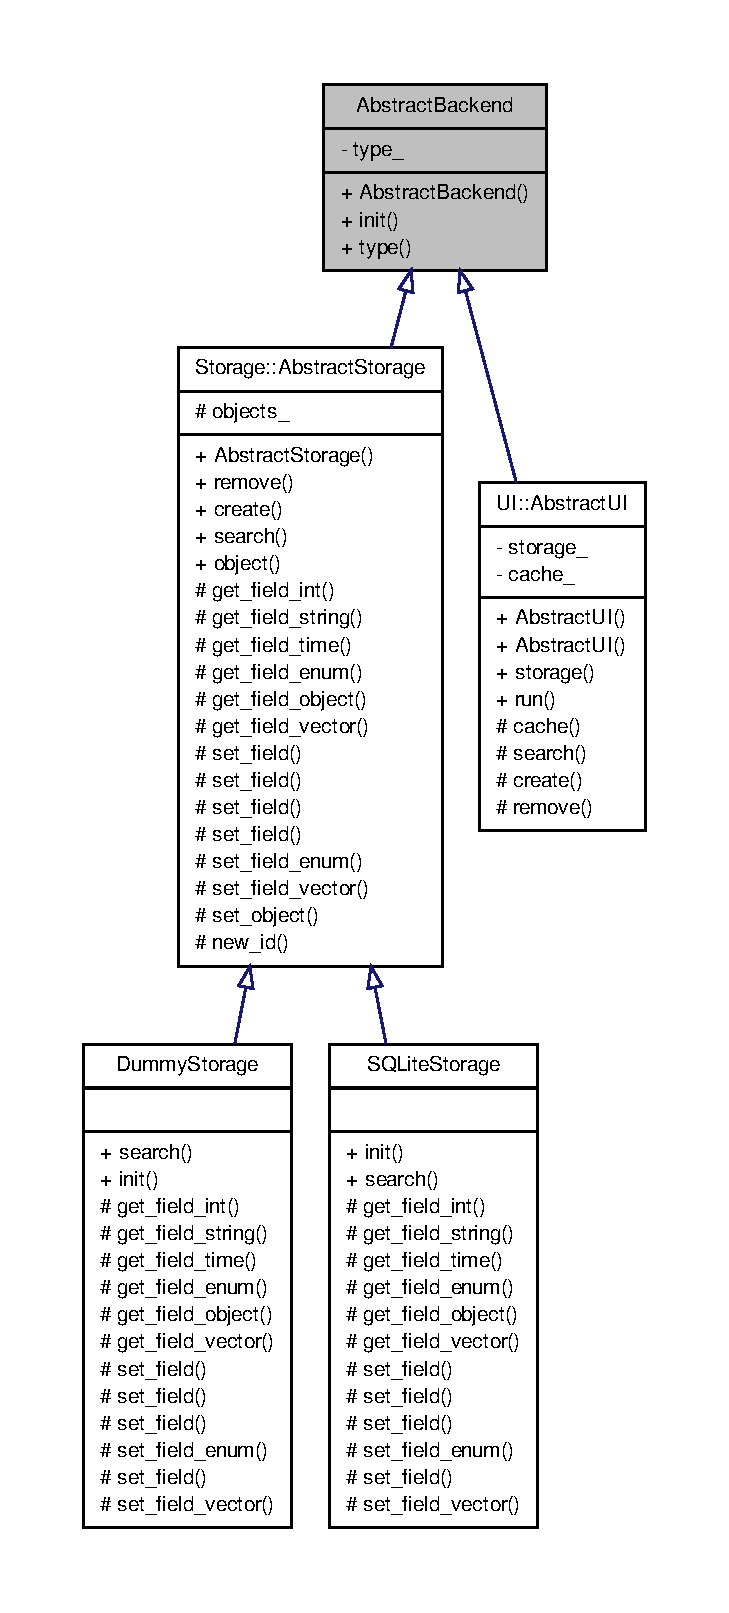
\includegraphics[height=600pt]{d7/dd9/classAbstractBackend__inherit__graph}
\end{center}
\end{figure}
\subsection*{Public Types}
\begin{DoxyCompactItemize}
\item 
enum \hyperlink{classAbstractBackend_a09da2d2fbf0862fb2af3928b438535d2}{Type} \{ \hyperlink{classAbstractBackend_a09da2d2fbf0862fb2af3928b438535d2ac0a0df2995db93384337b95598559a36}{STORAGE}, 
\hyperlink{classAbstractBackend_a09da2d2fbf0862fb2af3928b438535d2adcd5d3a3c71967aa82d09038477173ba}{UI}
 \}
\end{DoxyCompactItemize}
\subsection*{Public Member Functions}
\begin{DoxyCompactItemize}
\item 
\hyperlink{classAbstractBackend_ad91e2394ca45125ab197a15056e6a628}{AbstractBackend} (const enum \hyperlink{classAbstractBackend_a09da2d2fbf0862fb2af3928b438535d2}{Type} type)
\item 
virtual void \hyperlink{classAbstractBackend_afce49841a79e3093a1fbf199bfd9f698}{init} (const std::vector$<$ std::string $>$ \&args)=0
\item 
const \hyperlink{classAbstractBackend_a09da2d2fbf0862fb2af3928b438535d2}{Type} \hyperlink{classAbstractBackend_ae4f1fd32e7cff9d9d86e7b9fc6852668}{type} () const   throw ()
\end{DoxyCompactItemize}


\subsection{Member Enumeration Documentation}
\hypertarget{classAbstractBackend_a09da2d2fbf0862fb2af3928b438535d2}{
\index{AbstractBackend@{AbstractBackend}!Type@{Type}}
\index{Type@{Type}!AbstractBackend@{AbstractBackend}}
\subsubsection[{Type}]{\setlength{\rightskip}{0pt plus 5cm}enum {\bf AbstractBackend::Type}}}
\label{db/d37/classAbstractBackend_a09da2d2fbf0862fb2af3928b438535d2}
\begin{Desc}
\item[Enumerator: ]\par
\begin{description}
\index{STORAGE@{STORAGE}!AbstractBackend@{AbstractBackend}}\index{AbstractBackend@{AbstractBackend}!STORAGE@{STORAGE}}\item[{\em 
\hypertarget{classAbstractBackend_a09da2d2fbf0862fb2af3928b438535d2ac0a0df2995db93384337b95598559a36}{
STORAGE}
\label{db/d37/classAbstractBackend_a09da2d2fbf0862fb2af3928b438535d2ac0a0df2995db93384337b95598559a36}
}]\index{UI@{UI}!AbstractBackend@{AbstractBackend}}\index{AbstractBackend@{AbstractBackend}!UI@{UI}}\item[{\em 
\hypertarget{classAbstractBackend_a09da2d2fbf0862fb2af3928b438535d2adcd5d3a3c71967aa82d09038477173ba}{
UI}
\label{db/d37/classAbstractBackend_a09da2d2fbf0862fb2af3928b438535d2adcd5d3a3c71967aa82d09038477173ba}
}]\end{description}
\end{Desc}



\subsection{Constructor \& Destructor Documentation}
\hypertarget{classAbstractBackend_ad91e2394ca45125ab197a15056e6a628}{
\index{AbstractBackend@{AbstractBackend}!AbstractBackend@{AbstractBackend}}
\index{AbstractBackend@{AbstractBackend}!AbstractBackend@{AbstractBackend}}
\subsubsection[{AbstractBackend}]{\setlength{\rightskip}{0pt plus 5cm}AbstractBackend::AbstractBackend (
\begin{DoxyParamCaption}
\item[{const enum {\bf Type}}]{type}
\end{DoxyParamCaption}
)}}
\label{db/d37/classAbstractBackend_ad91e2394ca45125ab197a15056e6a628}


Here is the call graph for this function:
\nopagebreak
\begin{figure}[H]
\begin{center}
\leavevmode
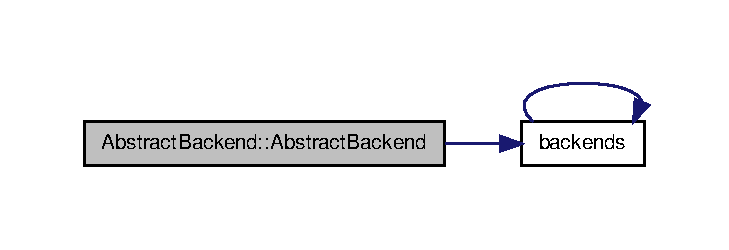
\includegraphics[width=350pt]{db/d37/classAbstractBackend_ad91e2394ca45125ab197a15056e6a628_cgraph}
\end{center}
\end{figure}




\subsection{Member Function Documentation}
\hypertarget{classAbstractBackend_afce49841a79e3093a1fbf199bfd9f698}{
\index{AbstractBackend@{AbstractBackend}!init@{init}}
\index{init@{init}!AbstractBackend@{AbstractBackend}}
\subsubsection[{init}]{\setlength{\rightskip}{0pt plus 5cm}virtual void AbstractBackend::init (
\begin{DoxyParamCaption}
\item[{const std::vector$<$ std::string $>$ \&}]{args}
\end{DoxyParamCaption}
)\hspace{0.3cm}{\ttfamily  \mbox{[}pure virtual\mbox{]}}}}
\label{db/d37/classAbstractBackend_afce49841a79e3093a1fbf199bfd9f698}


Implemented in \hyperlink{classSQLiteStorage_a1abd27f3824567fef222479a7c7a2333}{SQLiteStorage}, and \hyperlink{classDummyStorage_ac52f6e7c6941108e4686f606a4d88d6b}{DummyStorage}.



Here is the caller graph for this function:
\nopagebreak
\begin{figure}[H]
\begin{center}
\leavevmode
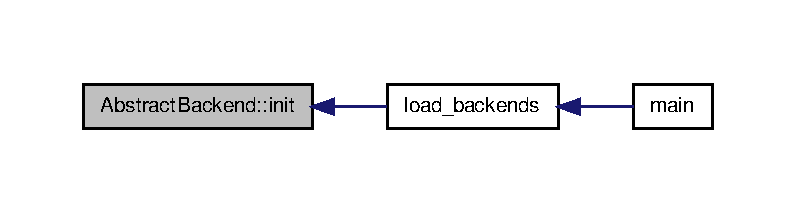
\includegraphics[width=382pt]{db/d37/classAbstractBackend_afce49841a79e3093a1fbf199bfd9f698_icgraph}
\end{center}
\end{figure}


\hypertarget{classAbstractBackend_ae4f1fd32e7cff9d9d86e7b9fc6852668}{
\index{AbstractBackend@{AbstractBackend}!type@{type}}
\index{type@{type}!AbstractBackend@{AbstractBackend}}
\subsubsection[{type}]{\setlength{\rightskip}{0pt plus 5cm}const {\bf Type} AbstractBackend::type (
\begin{DoxyParamCaption}
{}
\end{DoxyParamCaption}
) const  throw ()\hspace{0.3cm}{\ttfamily  \mbox{[}inline\mbox{]}}}}
\label{db/d37/classAbstractBackend_ae4f1fd32e7cff9d9d86e7b9fc6852668}


The documentation for this class was generated from the following files:\begin{DoxyCompactItemize}
\item 
src/include/\hyperlink{backend_8h}{backend.h}\item 
src/\hyperlink{backend_8cpp}{backend.cpp}\end{DoxyCompactItemize}

\hypertarget{classCore_1_1AbstractGroup}{
\section{Core::AbstractGroup Class Reference}
\label{dd/d68/classCore_1_1AbstractGroup}\index{Core::AbstractGroup@{Core::AbstractGroup}}
}


Base group functionality. You need to use it instead of \hyperlink{classCore_1_1Group}{Group} or \hyperlink{classCore_1_1Event}{Event} in most cases.  




{\ttfamily \#include $<$abstractgroup.h$>$}



Inheritance diagram for Core::AbstractGroup:
\nopagebreak
\begin{figure}[H]
\begin{center}
\leavevmode
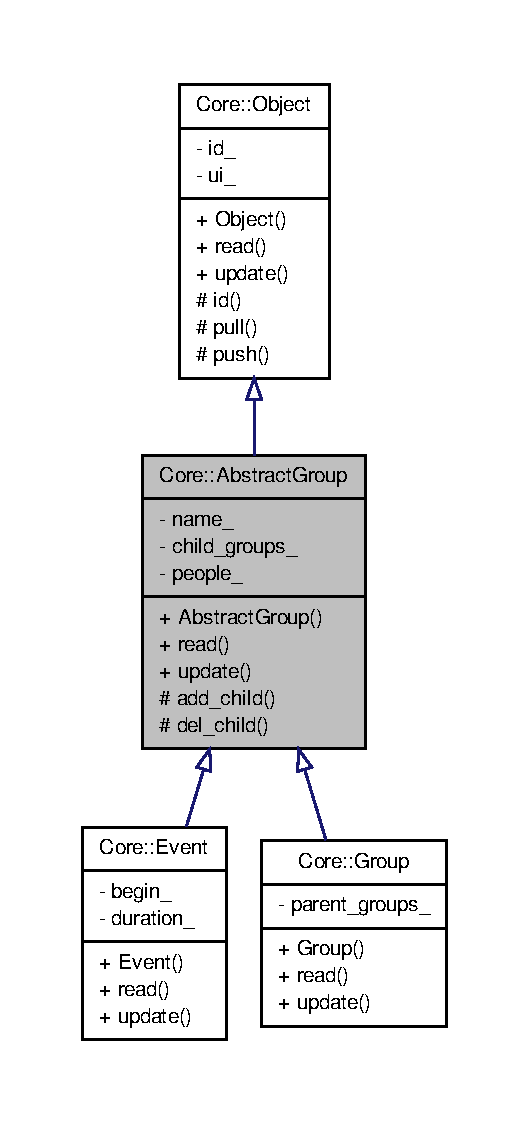
\includegraphics[width=254pt]{d2/d03/classCore_1_1AbstractGroup__inherit__graph}
\end{center}
\end{figure}


Collaboration diagram for Core::AbstractGroup:
\nopagebreak
\begin{figure}[H]
\begin{center}
\leavevmode
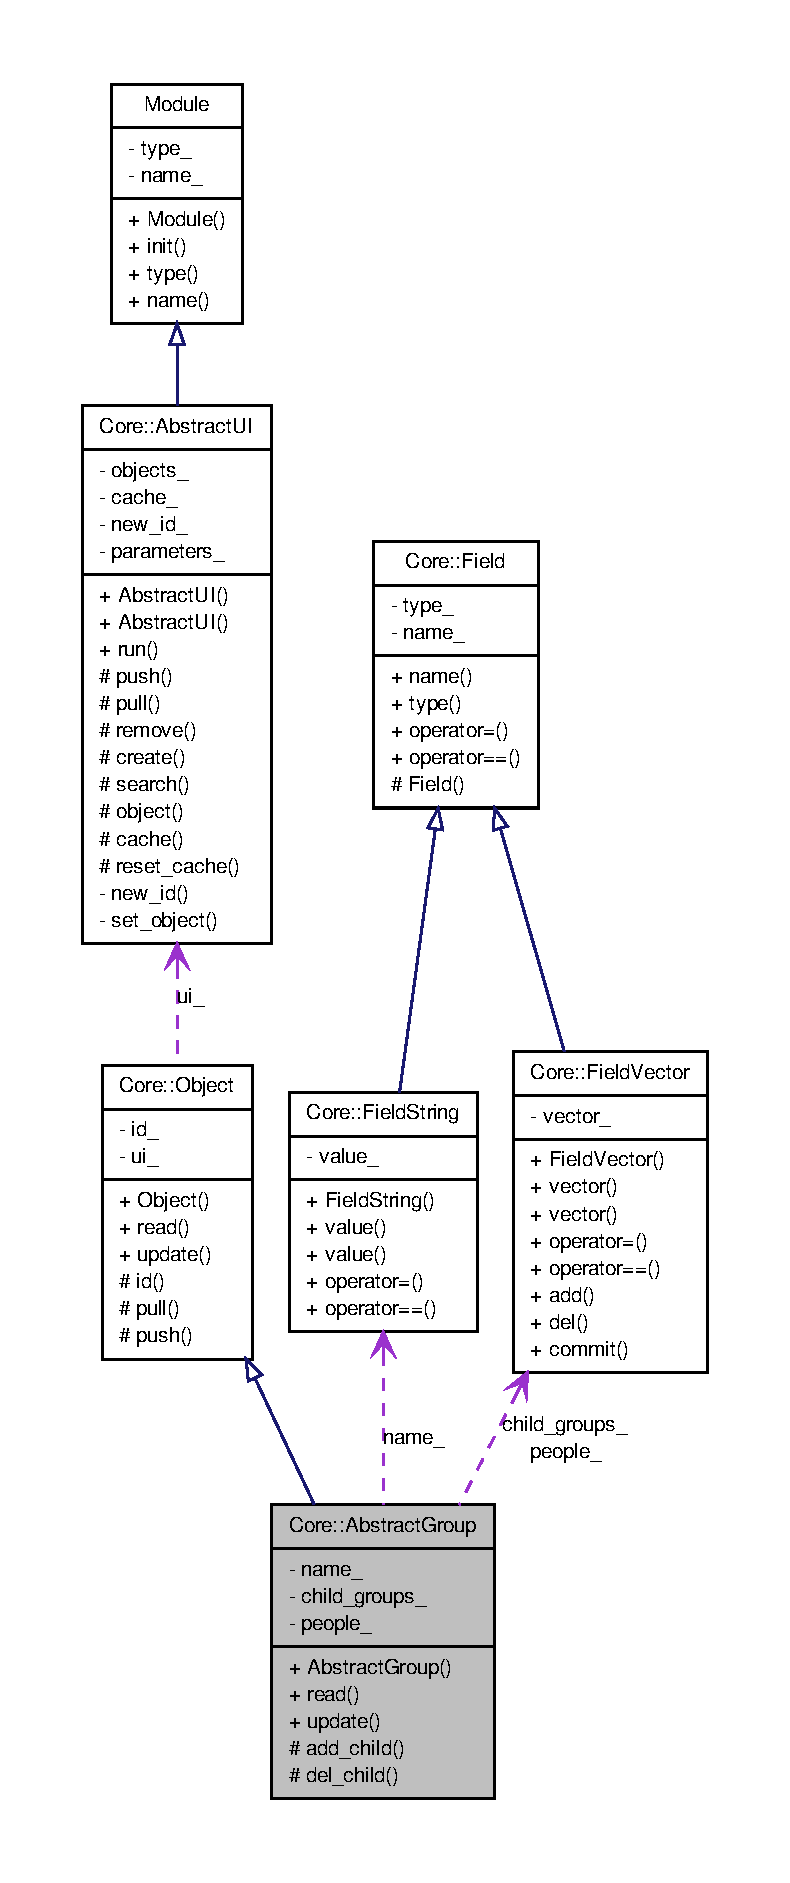
\includegraphics[height=600pt]{dd/dad/classCore_1_1AbstractGroup__coll__graph}
\end{center}
\end{figure}
\subsection*{Public Member Functions}
\begin{DoxyCompactItemize}
\item 
\hyperlink{classCore_1_1AbstractGroup_a413d72742d0f92f44615dba99e3430fd}{AbstractGroup} (const int id, \hyperlink{classCore_1_1AbstractUI}{AbstractUI} \&ui)  throw (std::bad\_\-cast)
\begin{DoxyCompactList}\small\item\em Constructor. \item\end{DoxyCompactList}\item 
virtual const \hyperlink{classCore_1_1Field}{Field} \& \hyperlink{classCore_1_1AbstractGroup_afd7a53d0bc49a5dbdc15505a686fca3d}{read} (const std::string \&name) const   throw (std::bad\_\-cast)
\item 
virtual void \hyperlink{classCore_1_1AbstractGroup_a397f639a0ee32efbc5a3ead8002745d5}{update} (const \hyperlink{classCore_1_1Field}{Field} \&field)  throw (std::bad\_\-cast)
\end{DoxyCompactItemize}
\subsection*{Protected Member Functions}
\begin{DoxyCompactItemize}
\item 
void \hyperlink{classCore_1_1AbstractGroup_aef90e91087aa5fcf4a94f0f2677f8f56}{add\_\-child} (\hyperlink{classCore_1_1AbstractGroup}{AbstractGroup} $\ast$group)
\begin{DoxyCompactList}\small\item\em Add child group to this one. \item\end{DoxyCompactList}\item 
void \hyperlink{classCore_1_1AbstractGroup_aa81866b9c414c24d25ca26311b4b4330}{del\_\-child} (\hyperlink{classCore_1_1AbstractGroup}{AbstractGroup} $\ast$group)
\begin{DoxyCompactList}\small\item\em Delete child group from this one. \item\end{DoxyCompactList}\end{DoxyCompactItemize}
\subsection*{Friends}
\begin{DoxyCompactItemize}
\item 
class \hyperlink{classCore_1_1AbstractGroup_a2697825715974a353728f0d4d5658112}{Group}
\end{DoxyCompactItemize}


\subsection{Detailed Description}
Base group functionality. You need to use it instead of \hyperlink{classCore_1_1Group}{Group} or \hyperlink{classCore_1_1Event}{Event} in most cases. This is a generalization of groups and events. It allows to work easy with them. It have not parent group as an \hyperlink{classCore_1_1Event}{Event}, but \hyperlink{classCore_1_1Group}{Group} have. 

\subsection{Constructor \& Destructor Documentation}
\hypertarget{classCore_1_1AbstractGroup_a413d72742d0f92f44615dba99e3430fd}{
\index{Core::AbstractGroup@{Core::AbstractGroup}!AbstractGroup@{AbstractGroup}}
\index{AbstractGroup@{AbstractGroup}!Core::AbstractGroup@{Core::AbstractGroup}}
\subsubsection[{AbstractGroup}]{\setlength{\rightskip}{0pt plus 5cm}AbstractGroup::AbstractGroup (
\begin{DoxyParamCaption}
\item[{const int}]{id, }
\item[{{\bf AbstractUI} \&}]{ui}
\end{DoxyParamCaption}
)  throw (std::bad\_\-cast)}}
\label{dd/d68/classCore_1_1AbstractGroup_a413d72742d0f92f44615dba99e3430fd}


Constructor. 


\begin{DoxyParams}[1]{Parameters}
\mbox{\tt in}  & {\em id} & AbstractUIs object`s identificator. \\
\hline
\mbox{\tt in}  & {\em ui} & Storage. \\
\hline
\end{DoxyParams}


\subsection{Member Function Documentation}
\hypertarget{classCore_1_1AbstractGroup_aef90e91087aa5fcf4a94f0f2677f8f56}{
\index{Core::AbstractGroup@{Core::AbstractGroup}!add\_\-child@{add\_\-child}}
\index{add\_\-child@{add\_\-child}!Core::AbstractGroup@{Core::AbstractGroup}}
\subsubsection[{add\_\-child}]{\setlength{\rightskip}{0pt plus 5cm}void AbstractGroup::add\_\-child (
\begin{DoxyParamCaption}
\item[{{\bf AbstractGroup} $\ast$}]{group}
\end{DoxyParamCaption}
)\hspace{0.3cm}{\ttfamily  \mbox{[}protected\mbox{]}}}}
\label{dd/d68/classCore_1_1AbstractGroup_aef90e91087aa5fcf4a94f0f2677f8f56}


Add child group to this one. 


\begin{DoxyParams}[1]{Parameters}
\mbox{\tt in}  & {\em group} & \hyperlink{classCore_1_1Group}{Group} to add. \\
\hline
\end{DoxyParams}


Here is the call graph for this function:
\nopagebreak
\begin{figure}[H]
\begin{center}
\leavevmode
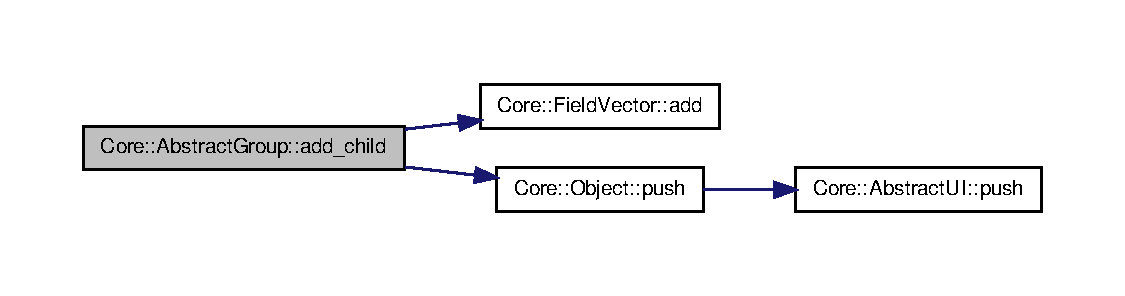
\includegraphics[width=400pt]{dd/d68/classCore_1_1AbstractGroup_aef90e91087aa5fcf4a94f0f2677f8f56_cgraph}
\end{center}
\end{figure}


\hypertarget{classCore_1_1AbstractGroup_aa81866b9c414c24d25ca26311b4b4330}{
\index{Core::AbstractGroup@{Core::AbstractGroup}!del\_\-child@{del\_\-child}}
\index{del\_\-child@{del\_\-child}!Core::AbstractGroup@{Core::AbstractGroup}}
\subsubsection[{del\_\-child}]{\setlength{\rightskip}{0pt plus 5cm}void AbstractGroup::del\_\-child (
\begin{DoxyParamCaption}
\item[{{\bf AbstractGroup} $\ast$}]{group}
\end{DoxyParamCaption}
)\hspace{0.3cm}{\ttfamily  \mbox{[}protected\mbox{]}}}}
\label{dd/d68/classCore_1_1AbstractGroup_aa81866b9c414c24d25ca26311b4b4330}


Delete child group from this one. 


\begin{DoxyParams}[1]{Parameters}
\mbox{\tt in}  & {\em group} & \hyperlink{classCore_1_1Group}{Group} to delete.  For use in \hyperlink{classCore_1_1Group_a9878d4ec0b02890502c6cff69da1e332}{Core::Group::update} method only.\\
\hline
\end{DoxyParams}
You must not use this method directly Use update methods instead. 

Here is the call graph for this function:
\nopagebreak
\begin{figure}[H]
\begin{center}
\leavevmode
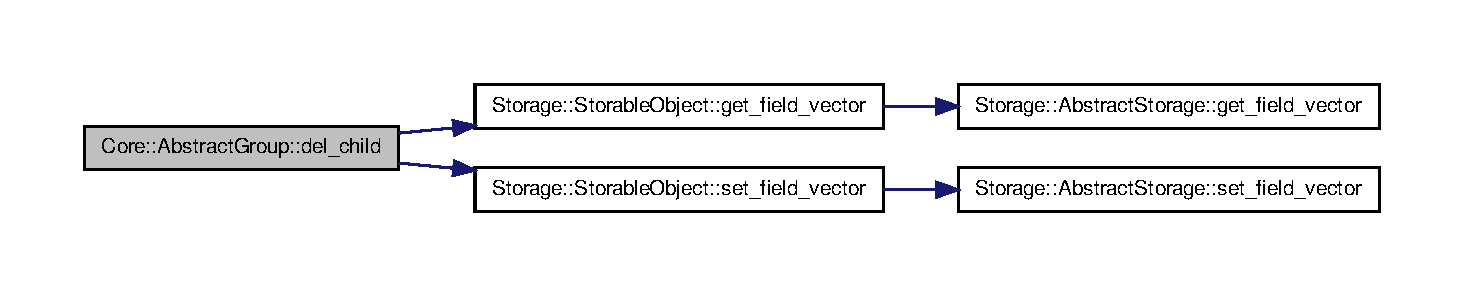
\includegraphics[width=400pt]{dd/d68/classCore_1_1AbstractGroup_aa81866b9c414c24d25ca26311b4b4330_cgraph}
\end{center}
\end{figure}


\hypertarget{classCore_1_1AbstractGroup_afd7a53d0bc49a5dbdc15505a686fca3d}{
\index{Core::AbstractGroup@{Core::AbstractGroup}!read@{read}}
\index{read@{read}!Core::AbstractGroup@{Core::AbstractGroup}}
\subsubsection[{read}]{\setlength{\rightskip}{0pt plus 5cm}const {\bf Field} \& AbstractGroup::read (
\begin{DoxyParamCaption}
\item[{const std::string \&}]{name}
\end{DoxyParamCaption}
) const  throw (std::bad\_\-cast)\hspace{0.3cm}{\ttfamily  \mbox{[}virtual\mbox{]}}}}
\label{dd/d68/classCore_1_1AbstractGroup_afd7a53d0bc49a5dbdc15505a686fca3d}
Get field of the object. 


\begin{DoxyParams}[1]{Parameters}
\mbox{\tt in}  & {\em name} & Name of the field to get. \\
\hline
\end{DoxyParams}
\begin{DoxyReturn}{Returns}
Corresponding field. 
\end{DoxyReturn}
 Get values of fields with those names: \char`\"{}name\char`\"{}, \char`\"{}people\char`\"{}, \char`\"{}child\_\-groups\char`\"{}.

Method returns object of \hyperlink{classCore_1_1FieldString}{Core::FieldString} or \hyperlink{classCore_1_1FieldVector}{Core::FieldVector} types. 

Implements \hyperlink{classCore_1_1Object_a90137d9981bd680bd395460e643c6560}{Core::Object}.



Reimplemented in \hyperlink{classCore_1_1Event_ac78ff90453b84d3342971772bba5c265}{Core::Event}, and \hyperlink{classCore_1_1Group_a0f4f5f00e11faeaaf09600d5b4943012}{Core::Group}.



Here is the caller graph for this function:
\nopagebreak
\begin{figure}[H]
\begin{center}
\leavevmode
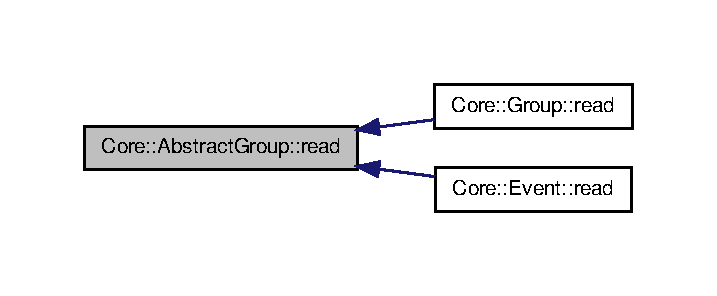
\includegraphics[width=344pt]{dd/d68/classCore_1_1AbstractGroup_afd7a53d0bc49a5dbdc15505a686fca3d_icgraph}
\end{center}
\end{figure}


\hypertarget{classCore_1_1AbstractGroup_a397f639a0ee32efbc5a3ead8002745d5}{
\index{Core::AbstractGroup@{Core::AbstractGroup}!update@{update}}
\index{update@{update}!Core::AbstractGroup@{Core::AbstractGroup}}
\subsubsection[{update}]{\setlength{\rightskip}{0pt plus 5cm}void AbstractGroup::update (
\begin{DoxyParamCaption}
\item[{const {\bf Field} \&}]{field}
\end{DoxyParamCaption}
)  throw (std::bad\_\-cast)\hspace{0.3cm}{\ttfamily  \mbox{[}virtual\mbox{]}}}}
\label{dd/d68/classCore_1_1AbstractGroup_a397f639a0ee32efbc5a3ead8002745d5}
Change field of the object. 


\begin{DoxyParams}[1]{Parameters}
\mbox{\tt in}  & {\em field} & \hyperlink{classCore_1_1Field}{Field} to change. \\
\hline
\end{DoxyParams}
 Change values of fields with those names: \char`\"{}name\char`\"{}, \char`\"{}people\char`\"{}, \char`\"{}child\_\-groups\char`\"{}.

Methods accepts object of \hyperlink{classCore_1_1FieldString}{Core::FieldString}, \hyperlink{classCore_1_1FieldLink}{Core::FieldLink} or \hyperlink{classCore_1_1FieldVector}{Core::FieldVector} types. 

Implements \hyperlink{classCore_1_1Object_a53328d659235e29f418ff4890cc3bdb3}{Core::Object}.



Reimplemented in \hyperlink{classCore_1_1Event_a8e147f35e8ee4fd0891a290424b098d3}{Core::Event}, and \hyperlink{classCore_1_1Group_a9878d4ec0b02890502c6cff69da1e332}{Core::Group}.



Here is the caller graph for this function:
\nopagebreak
\begin{figure}[H]
\begin{center}
\leavevmode
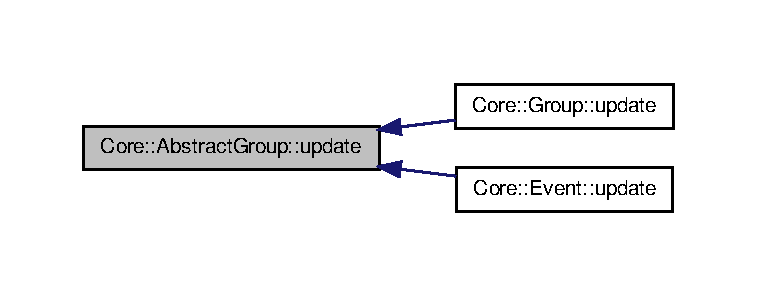
\includegraphics[width=364pt]{dd/d68/classCore_1_1AbstractGroup_a397f639a0ee32efbc5a3ead8002745d5_icgraph}
\end{center}
\end{figure}




\subsection{Friends And Related Function Documentation}
\hypertarget{classCore_1_1AbstractGroup_a2697825715974a353728f0d4d5658112}{
\index{Core::AbstractGroup@{Core::AbstractGroup}!Group@{Group}}
\index{Group@{Group}!Core::AbstractGroup@{Core::AbstractGroup}}
\subsubsection[{Group}]{\setlength{\rightskip}{0pt plus 5cm}friend class {\bf Group}\hspace{0.3cm}{\ttfamily  \mbox{[}friend\mbox{]}}}}
\label{dd/d68/classCore_1_1AbstractGroup_a2697825715974a353728f0d4d5658112}


The documentation for this class was generated from the following files:\begin{DoxyCompactItemize}
\item 
src/include/\hyperlink{abstractgroup_8h}{abstractgroup.h}\item 
src/core/\hyperlink{abstractgroup_8cpp}{abstractgroup.cpp}\end{DoxyCompactItemize}

\hypertarget{classStorage_1_1AbstractStorage}{
\section{Storage::AbstractStorage Class Reference}
\label{d6/da0/classStorage_1_1AbstractStorage}\index{Storage::AbstractStorage@{Storage::AbstractStorage}}
}


Abstract interface for storage.  




{\ttfamily \#include $<$abstractstorage.h$>$}



Inheritance diagram for Storage::AbstractStorage:
\nopagebreak
\begin{figure}[H]
\begin{center}
\leavevmode
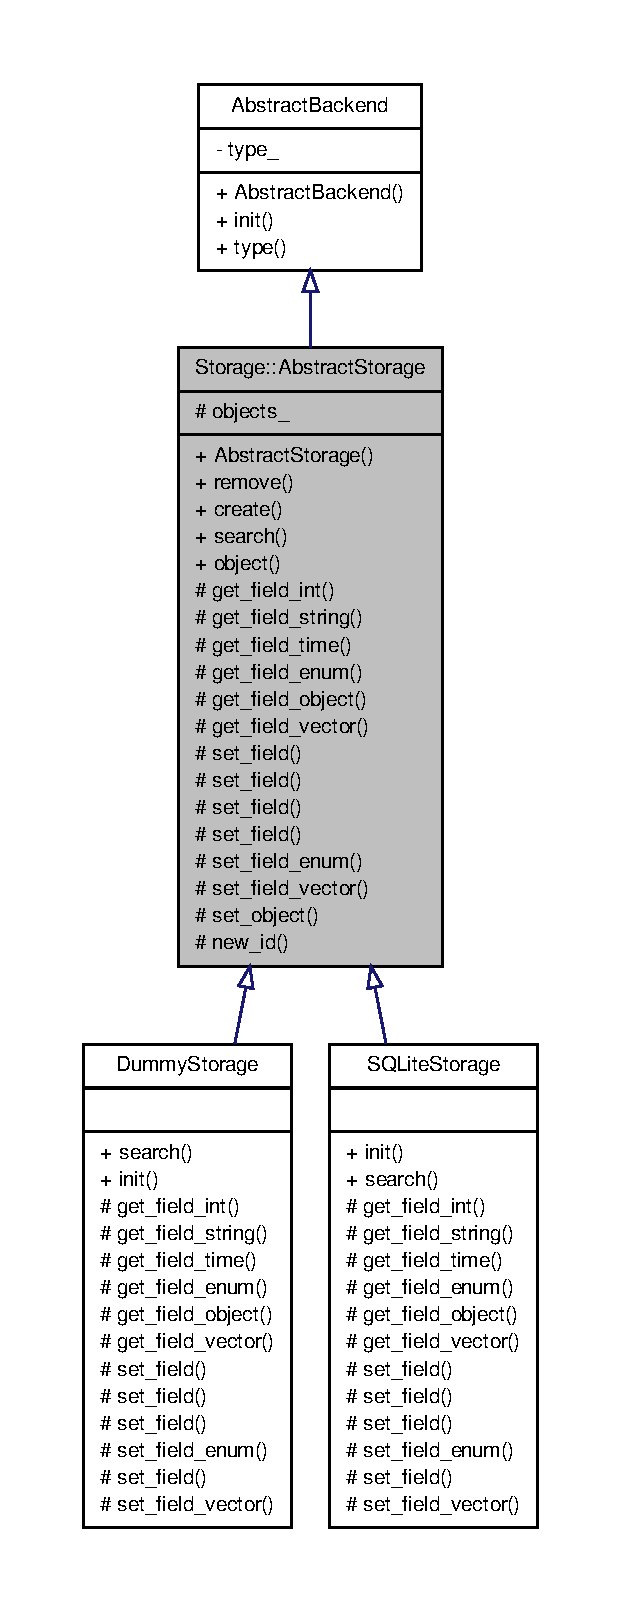
\includegraphics[height=600pt]{d9/db4/classStorage_1_1AbstractStorage__inherit__graph}
\end{center}
\end{figure}


Collaboration diagram for Storage::AbstractStorage:
\nopagebreak
\begin{figure}[H]
\begin{center}
\leavevmode
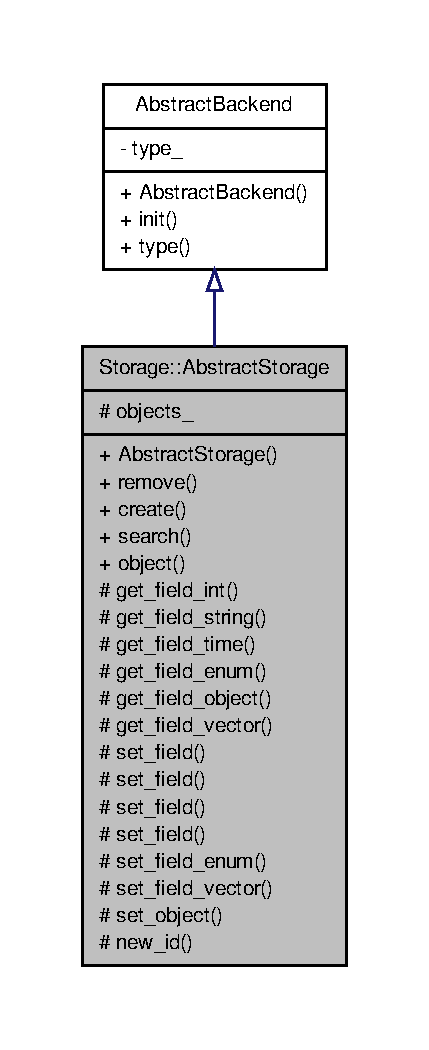
\includegraphics[width=206pt]{db/d69/classStorage_1_1AbstractStorage__coll__graph}
\end{center}
\end{figure}
\subsection*{Classes}
\begin{DoxyCompactItemize}
\item 
struct \hyperlink{structStorage_1_1AbstractStorage_1_1Argument}{Argument}
\begin{DoxyCompactList}\small\item\em an auxiliary structure to make search query and create objects. \item\end{DoxyCompactList}\end{DoxyCompactItemize}
\subsection*{Public Member Functions}
\begin{DoxyCompactItemize}
\item 
\hyperlink{classStorage_1_1AbstractStorage_a73fd0acd5b0f71febf5254db391416c0}{AbstractStorage} ()
\begin{DoxyCompactList}\small\item\em Constructor. \item\end{DoxyCompactList}\item 
virtual void \hyperlink{classStorage_1_1AbstractStorage_a5d114117d4954e01fd650251b829fdbf}{remove} (\hyperlink{classStorage_1_1StorableObject}{StorableObject} $\ast$object)
\begin{DoxyCompactList}\small\item\em Remove object from the storage. \item\end{DoxyCompactList}\item 
{\footnotesize template$<$class T $>$ }\\\hyperlink{classStorage_1_1StorableObject}{StorableObject} $\ast$ \hyperlink{classStorage_1_1AbstractStorage_a108af124f19c0ae9a4a461aee6abc3ec}{create} (std::vector$<$ const \hyperlink{structStorage_1_1AbstractStorage_1_1Argument}{Argument} $\ast$ $>$ \&parameters)
\item 
virtual std::vector$<$ \hyperlink{classStorage_1_1StorableObject}{StorableObject} $\ast$ $>$ $\ast$ \hyperlink{classStorage_1_1AbstractStorage_a9304eea8cd6fffd77b1ccd26f85a061c}{search} (std::vector$<$ \hyperlink{structStorage_1_1AbstractStorage_1_1Argument}{Argument} $\ast$ $>$ \&parameters)=0
\begin{DoxyCompactList}\small\item\em Search objects by some parameters. \item\end{DoxyCompactList}\item 
virtual \hyperlink{classStorage_1_1StorableObject}{StorableObject} $\ast$ \hyperlink{classStorage_1_1AbstractStorage_a21ff57c954664abb78d1d658a1da7afa}{object} (const int id) const   throw (std::bad\_\-cast)
\begin{DoxyCompactList}\small\item\em Return object by id. \item\end{DoxyCompactList}\end{DoxyCompactItemize}
\subsection*{Protected Member Functions}
\begin{DoxyCompactItemize}
\item 
virtual const int \hyperlink{classStorage_1_1AbstractStorage_a80a7e4ab87a0326aa8b5571b09d55eaa}{get\_\-field\_\-int} (const int id, const std::string field) const =0  throw (std::bad\_\-cast)
\begin{DoxyCompactList}\small\item\em Return integer value of requested field. \item\end{DoxyCompactList}\item 
virtual const std::string \hyperlink{classStorage_1_1AbstractStorage_ad12a3abb791ef5a696196c28e643ec22}{get\_\-field\_\-string} (const int id, const std::string field) const =0  throw (std::bad\_\-cast)
\begin{DoxyCompactList}\small\item\em Return string value of requested field. \item\end{DoxyCompactList}\item 
virtual const time\_\-t \hyperlink{classStorage_1_1AbstractStorage_a87fe8d51934ab2403758d905ef313272}{get\_\-field\_\-time} (const int id, const std::string field) const =0  throw (std::bad\_\-cast)
\begin{DoxyCompactList}\small\item\em Return time value of requested field. \item\end{DoxyCompactList}\item 
virtual const std::string \hyperlink{classStorage_1_1AbstractStorage_acd7e88a005b6873632c7f20245e5f3f7}{get\_\-field\_\-enum} (const int id, const std::string field) const =0  throw (std::bad\_\-cast)
\begin{DoxyCompactList}\small\item\em Return enum value of requested field. \item\end{DoxyCompactList}\item 
virtual \hyperlink{classStorage_1_1StorableObject}{StorableObject} $\ast$ \hyperlink{classStorage_1_1AbstractStorage_aaff107d1f51e456f26c03861beb0fff7}{get\_\-field\_\-object} (const int id, const std::string field) const =0  throw (std::bad\_\-cast)
\begin{DoxyCompactList}\small\item\em Return object value of requested field. \item\end{DoxyCompactList}\item 
virtual const std::vector$<$ \hyperlink{classStorage_1_1StorableObject}{StorableObject} $\ast$ $>$ \hyperlink{classStorage_1_1AbstractStorage_ae7c30697d68dc9d7de595388030d8e10}{get\_\-field\_\-vector} (const int id, const std::string field) const =0  throw (std::bad\_\-cast)
\begin{DoxyCompactList}\small\item\em Return vector value of requested field. \item\end{DoxyCompactList}\item 
virtual void \hyperlink{classStorage_1_1AbstractStorage_acdd090d0beb6a8241914e7d78a7f2c0c}{set\_\-field} (const int id, const std::string field, const int value)=0  throw (std::bad\_\-cast)
\begin{DoxyCompactList}\small\item\em Set integer value of requested field. \item\end{DoxyCompactList}\item 
virtual void \hyperlink{classStorage_1_1AbstractStorage_ae5ee00e647f121b68ebada0f094058bc}{set\_\-field} (const int id, const std::string field, const std::string value)=0  throw (std::bad\_\-cast)
\begin{DoxyCompactList}\small\item\em Set string value of requested field. \item\end{DoxyCompactList}\item 
virtual void \hyperlink{classStorage_1_1AbstractStorage_a50ee4a829bc067a9291a11aa99ec0f16}{set\_\-field} (const int id, const std::string field, const time\_\-t value)=0  throw (std::bad\_\-cast)
\begin{DoxyCompactList}\small\item\em Set time value of requested field. \item\end{DoxyCompactList}\item 
virtual void \hyperlink{classStorage_1_1AbstractStorage_a7ef9f70b3fcbaa2863de2be695dc77c1}{set\_\-field} (const int id, const std::string field, \hyperlink{classStorage_1_1StorableObject}{StorableObject} $\ast$value)=0  throw (std::bad\_\-cast)
\begin{DoxyCompactList}\small\item\em Set object value of requested field. \item\end{DoxyCompactList}\item 
virtual void \hyperlink{classStorage_1_1AbstractStorage_a50925678c74c09acd8549a541fdbbe9f}{set\_\-field\_\-enum} (const int id, const std::string field, const std::string value)=0  throw (std::bad\_\-cast)
\begin{DoxyCompactList}\small\item\em Set enum value of requested field. \item\end{DoxyCompactList}\item 
virtual void \hyperlink{classStorage_1_1AbstractStorage_a24af03b9a68ace199b0a6fa812abad39}{set\_\-field\_\-vector} (const int id, const std::string field, const std::vector$<$ \hyperlink{classStorage_1_1StorableObject}{StorableObject} $\ast$ $>$ vector)=0  throw (std::bad\_\-cast)
\begin{DoxyCompactList}\small\item\em Set vector value of requested field. \item\end{DoxyCompactList}\item 
virtual void \hyperlink{classStorage_1_1AbstractStorage_a641a6b75fe34c51943902d846ff66328}{set\_\-object} (\hyperlink{classStorage_1_1StorableObject}{StorableObject} $\ast$object)
\begin{DoxyCompactList}\small\item\em Set integer value of requested field. \item\end{DoxyCompactList}\item 
virtual const int \hyperlink{classStorage_1_1AbstractStorage_ab9e323067a58b74a7d1c835f0d1832c8}{new\_\-id} ()
\begin{DoxyCompactList}\small\item\em Return new object identificator and reserve cell for it in the objects vector. \item\end{DoxyCompactList}\end{DoxyCompactItemize}
\subsection*{Protected Attributes}
\begin{DoxyCompactItemize}
\item 
std::vector$<$ \hyperlink{classStorage_1_1StorableObject}{StorableObject} $\ast$ $>$ \hyperlink{classStorage_1_1AbstractStorage_a54758736009f559baf85a2d477b4d370}{objects\_\-}
\end{DoxyCompactItemize}
\subsection*{Friends}
\begin{DoxyCompactItemize}
\item 
class \hyperlink{classStorage_1_1AbstractStorage_ac344c900799ce1069f4324f043f17763}{StorableObject}
\end{DoxyCompactItemize}


\subsection{Detailed Description}
Abstract interface for storage. Each storage backend must to inherit this class. It can be chahged later, it is too simple to work fast now. 

\subsection{Constructor \& Destructor Documentation}
\hypertarget{classStorage_1_1AbstractStorage_a73fd0acd5b0f71febf5254db391416c0}{
\index{Storage::AbstractStorage@{Storage::AbstractStorage}!AbstractStorage@{AbstractStorage}}
\index{AbstractStorage@{AbstractStorage}!Storage::AbstractStorage@{Storage::AbstractStorage}}
\subsubsection[{AbstractStorage}]{\setlength{\rightskip}{0pt plus 5cm}Storage::AbstractStorage::AbstractStorage (
\begin{DoxyParamCaption}
{}
\end{DoxyParamCaption}
)\hspace{0.3cm}{\ttfamily  \mbox{[}inline\mbox{]}}}}
\label{d6/da0/classStorage_1_1AbstractStorage_a73fd0acd5b0f71febf5254db391416c0}


Constructor. 



\subsection{Member Function Documentation}
\hypertarget{classStorage_1_1AbstractStorage_a108af124f19c0ae9a4a461aee6abc3ec}{
\index{Storage::AbstractStorage@{Storage::AbstractStorage}!create@{create}}
\index{create@{create}!Storage::AbstractStorage@{Storage::AbstractStorage}}
\subsubsection[{create}]{\setlength{\rightskip}{0pt plus 5cm}template$<$class T $>$ {\bf StorableObject}$\ast$ Storage::AbstractStorage::create (
\begin{DoxyParamCaption}
\item[{std::vector$<$ const {\bf Argument} $\ast$ $>$ \&}]{parameters}
\end{DoxyParamCaption}
)\hspace{0.3cm}{\ttfamily  \mbox{[}inline\mbox{]}}}}
\label{d6/da0/classStorage_1_1AbstractStorage_a108af124f19c0ae9a4a461aee6abc3ec}

\begin{DoxyParams}[1]{Parameters}
 & {\em parameters} & Create an object of the T type \\
\hline
\mbox{\tt in}  & {\em parameters} & new object`s data. \\
\hline
\end{DoxyParams}
\begin{DoxyReturn}{Returns}
pointer to the created object.
\end{DoxyReturn}
This method must be called from the user interface to create new object. 

Here is the call graph for this function:
\nopagebreak
\begin{figure}[H]
\begin{center}
\leavevmode
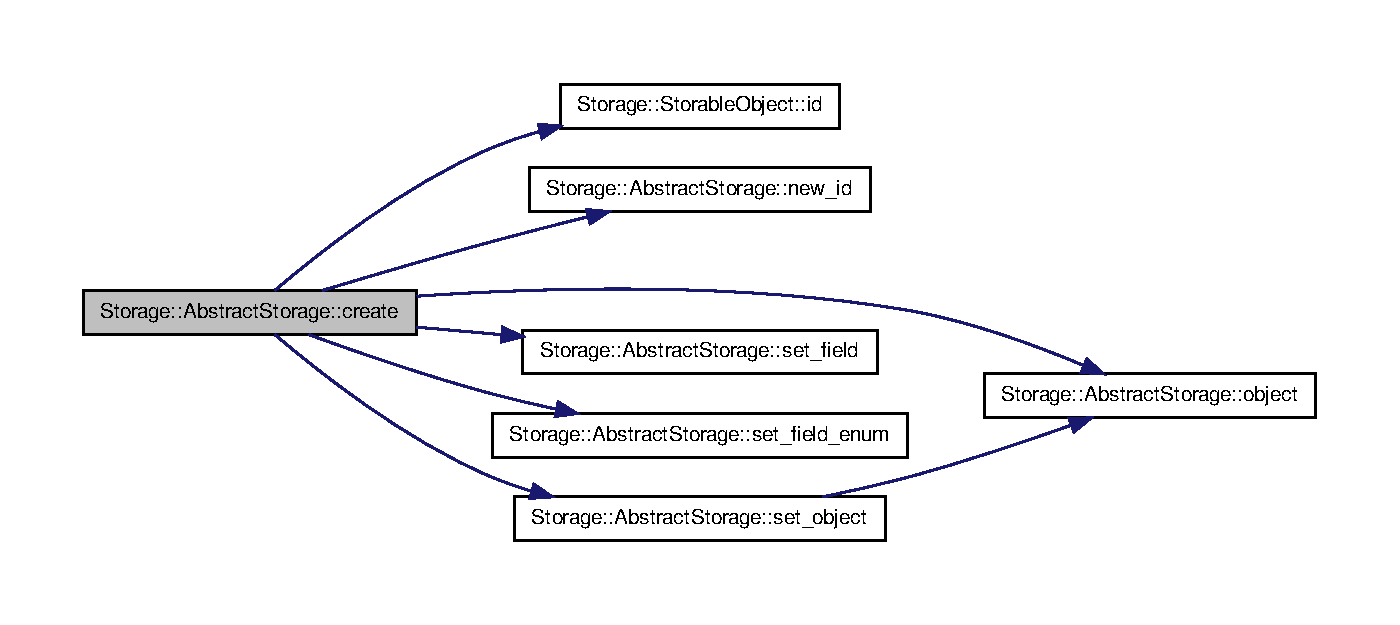
\includegraphics[width=400pt]{d6/da0/classStorage_1_1AbstractStorage_a108af124f19c0ae9a4a461aee6abc3ec_cgraph}
\end{center}
\end{figure}




Here is the caller graph for this function:
\nopagebreak
\begin{figure}[H]
\begin{center}
\leavevmode
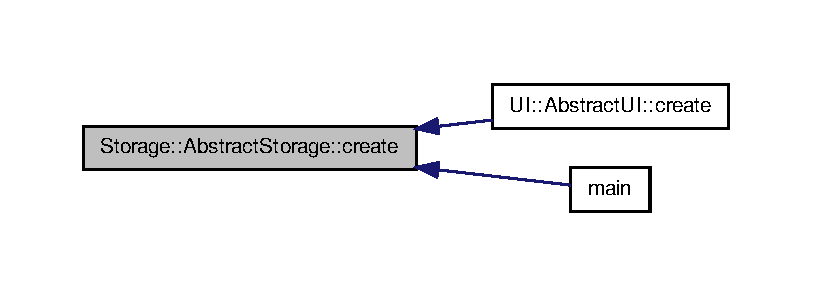
\includegraphics[width=390pt]{d6/da0/classStorage_1_1AbstractStorage_a108af124f19c0ae9a4a461aee6abc3ec_icgraph}
\end{center}
\end{figure}


\hypertarget{classStorage_1_1AbstractStorage_acd7e88a005b6873632c7f20245e5f3f7}{
\index{Storage::AbstractStorage@{Storage::AbstractStorage}!get\_\-field\_\-enum@{get\_\-field\_\-enum}}
\index{get\_\-field\_\-enum@{get\_\-field\_\-enum}!Storage::AbstractStorage@{Storage::AbstractStorage}}
\subsubsection[{get\_\-field\_\-enum}]{\setlength{\rightskip}{0pt plus 5cm}virtual const std::string Storage::AbstractStorage::get\_\-field\_\-enum (
\begin{DoxyParamCaption}
\item[{const int}]{id, }
\item[{const std::string}]{field}
\end{DoxyParamCaption}
) const  throw (std::bad\_\-cast)\hspace{0.3cm}{\ttfamily  \mbox{[}protected, pure virtual\mbox{]}}}}
\label{d6/da0/classStorage_1_1AbstractStorage_acd7e88a005b6873632c7f20245e5f3f7}


Return enum value of requested field. 


\begin{DoxyParams}[1]{Parameters}
\mbox{\tt in}  & {\em id} & Object identificator. \\
\hline
\mbox{\tt in}  & {\em field} & Field name. \\
\hline
\end{DoxyParams}
\begin{DoxyReturn}{Returns}
requested value.
\end{DoxyReturn}
This method must be realized in inherited classes. Throw an std::bad\_\-cast exception if requested field does not exists or keeped in another type. 

Implemented in \hyperlink{classSQLiteStorage_aef325b647f98c8e5fdb402ec608b403b}{SQLiteStorage}, and \hyperlink{classDummyStorage_a1101739c23fbf79b009558553180ef1a}{DummyStorage}.



Here is the caller graph for this function:
\nopagebreak
\begin{figure}[H]
\begin{center}
\leavevmode
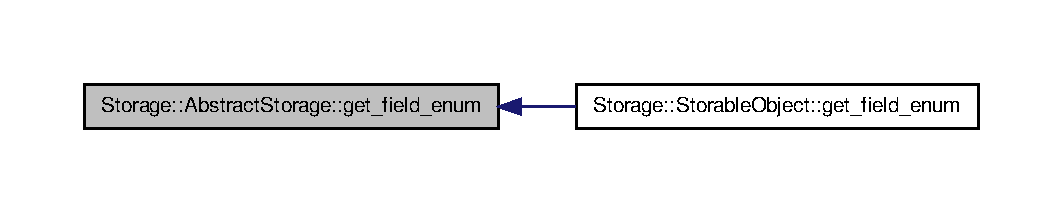
\includegraphics[width=400pt]{d6/da0/classStorage_1_1AbstractStorage_acd7e88a005b6873632c7f20245e5f3f7_icgraph}
\end{center}
\end{figure}


\hypertarget{classStorage_1_1AbstractStorage_a80a7e4ab87a0326aa8b5571b09d55eaa}{
\index{Storage::AbstractStorage@{Storage::AbstractStorage}!get\_\-field\_\-int@{get\_\-field\_\-int}}
\index{get\_\-field\_\-int@{get\_\-field\_\-int}!Storage::AbstractStorage@{Storage::AbstractStorage}}
\subsubsection[{get\_\-field\_\-int}]{\setlength{\rightskip}{0pt plus 5cm}virtual const int Storage::AbstractStorage::get\_\-field\_\-int (
\begin{DoxyParamCaption}
\item[{const int}]{id, }
\item[{const std::string}]{field}
\end{DoxyParamCaption}
) const  throw (std::bad\_\-cast)\hspace{0.3cm}{\ttfamily  \mbox{[}protected, pure virtual\mbox{]}}}}
\label{d6/da0/classStorage_1_1AbstractStorage_a80a7e4ab87a0326aa8b5571b09d55eaa}


Return integer value of requested field. 


\begin{DoxyParams}[1]{Parameters}
\mbox{\tt in}  & {\em id} & Object identificator. \\
\hline
\mbox{\tt in}  & {\em field} & Field name. \\
\hline
\end{DoxyParams}
\begin{DoxyReturn}{Returns}
requested value.
\end{DoxyReturn}
This method must be realized in inherited classes. Throw an std::bad\_\-cast exception if requested field does not exists or keeped in another type. 

Implemented in \hyperlink{classSQLiteStorage_aab5d70b4dbe29dbe6e9243a89ee81a89}{SQLiteStorage}, and \hyperlink{classDummyStorage_a275263eba82a652005292f01a120af8e}{DummyStorage}.



Here is the caller graph for this function:
\nopagebreak
\begin{figure}[H]
\begin{center}
\leavevmode
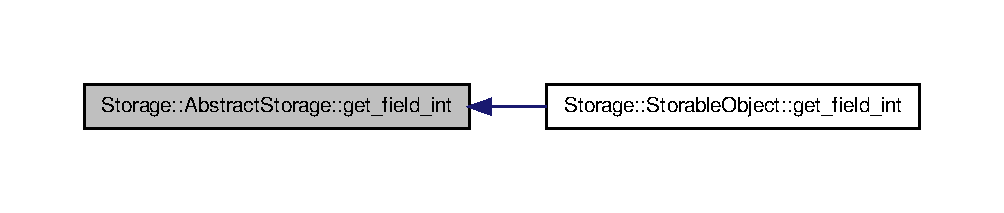
\includegraphics[width=400pt]{d6/da0/classStorage_1_1AbstractStorage_a80a7e4ab87a0326aa8b5571b09d55eaa_icgraph}
\end{center}
\end{figure}


\hypertarget{classStorage_1_1AbstractStorage_aaff107d1f51e456f26c03861beb0fff7}{
\index{Storage::AbstractStorage@{Storage::AbstractStorage}!get\_\-field\_\-object@{get\_\-field\_\-object}}
\index{get\_\-field\_\-object@{get\_\-field\_\-object}!Storage::AbstractStorage@{Storage::AbstractStorage}}
\subsubsection[{get\_\-field\_\-object}]{\setlength{\rightskip}{0pt plus 5cm}virtual {\bf StorableObject}$\ast$ Storage::AbstractStorage::get\_\-field\_\-object (
\begin{DoxyParamCaption}
\item[{const int}]{id, }
\item[{const std::string}]{field}
\end{DoxyParamCaption}
) const  throw (std::bad\_\-cast)\hspace{0.3cm}{\ttfamily  \mbox{[}protected, pure virtual\mbox{]}}}}
\label{d6/da0/classStorage_1_1AbstractStorage_aaff107d1f51e456f26c03861beb0fff7}


Return object value of requested field. 


\begin{DoxyParams}[1]{Parameters}
\mbox{\tt in}  & {\em id} & Object identificator. \\
\hline
\mbox{\tt in}  & {\em field} & Field name. \\
\hline
\end{DoxyParams}
\begin{DoxyReturn}{Returns}
requested value.
\end{DoxyReturn}
This method must be realized in inherited classes. Throw an std::bad\_\-cast exception if requested field does not exists or keeped in another type. 

Implemented in \hyperlink{classSQLiteStorage_adf1189839ae893f3ce4c73c3ee69634d}{SQLiteStorage}, and \hyperlink{classDummyStorage_a7135d171d9b83c2fbf72851fa9ea852a}{DummyStorage}.



Here is the caller graph for this function:
\nopagebreak
\begin{figure}[H]
\begin{center}
\leavevmode
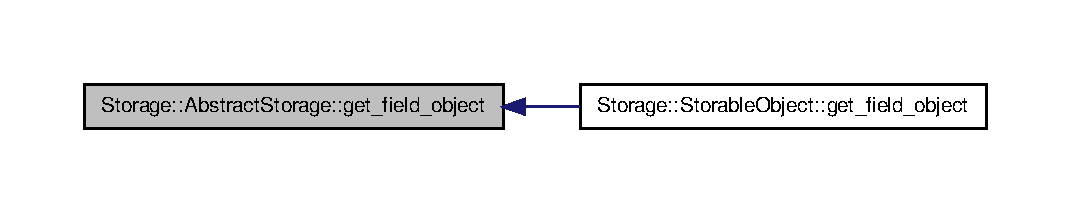
\includegraphics[width=400pt]{d6/da0/classStorage_1_1AbstractStorage_aaff107d1f51e456f26c03861beb0fff7_icgraph}
\end{center}
\end{figure}


\hypertarget{classStorage_1_1AbstractStorage_ad12a3abb791ef5a696196c28e643ec22}{
\index{Storage::AbstractStorage@{Storage::AbstractStorage}!get\_\-field\_\-string@{get\_\-field\_\-string}}
\index{get\_\-field\_\-string@{get\_\-field\_\-string}!Storage::AbstractStorage@{Storage::AbstractStorage}}
\subsubsection[{get\_\-field\_\-string}]{\setlength{\rightskip}{0pt plus 5cm}virtual const std::string Storage::AbstractStorage::get\_\-field\_\-string (
\begin{DoxyParamCaption}
\item[{const int}]{id, }
\item[{const std::string}]{field}
\end{DoxyParamCaption}
) const  throw (std::bad\_\-cast)\hspace{0.3cm}{\ttfamily  \mbox{[}protected, pure virtual\mbox{]}}}}
\label{d6/da0/classStorage_1_1AbstractStorage_ad12a3abb791ef5a696196c28e643ec22}


Return string value of requested field. 


\begin{DoxyParams}[1]{Parameters}
\mbox{\tt in}  & {\em id} & Object identificator. \\
\hline
\mbox{\tt in}  & {\em field} & Field name. \\
\hline
\end{DoxyParams}
\begin{DoxyReturn}{Returns}
requested value.
\end{DoxyReturn}
This method must be realized in inherited classes. Throw an std::bad\_\-cast exception if requested field does not exists or keeped in another type. 

Implemented in \hyperlink{classSQLiteStorage_a5a68da392583ef992a3aff78cfdacc8a}{SQLiteStorage}, and \hyperlink{classDummyStorage_a410ef9d239193e25f830c49140e18293}{DummyStorage}.



Here is the caller graph for this function:
\nopagebreak
\begin{figure}[H]
\begin{center}
\leavevmode
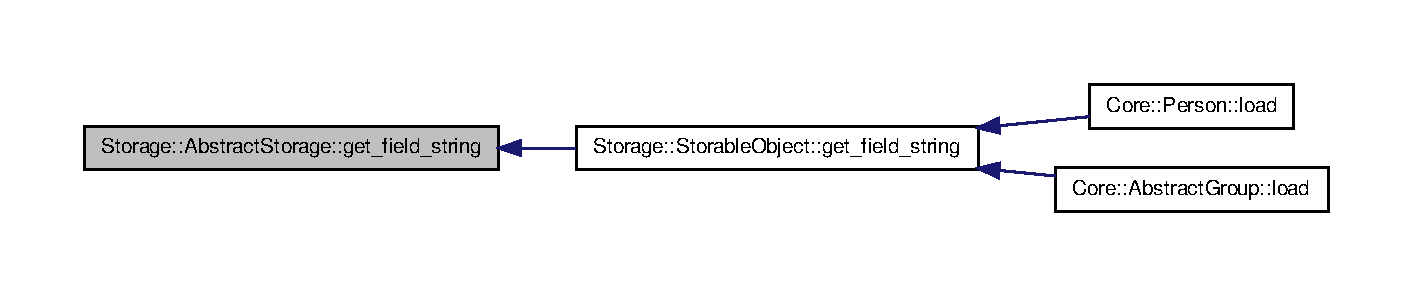
\includegraphics[width=400pt]{d6/da0/classStorage_1_1AbstractStorage_ad12a3abb791ef5a696196c28e643ec22_icgraph}
\end{center}
\end{figure}


\hypertarget{classStorage_1_1AbstractStorage_a87fe8d51934ab2403758d905ef313272}{
\index{Storage::AbstractStorage@{Storage::AbstractStorage}!get\_\-field\_\-time@{get\_\-field\_\-time}}
\index{get\_\-field\_\-time@{get\_\-field\_\-time}!Storage::AbstractStorage@{Storage::AbstractStorage}}
\subsubsection[{get\_\-field\_\-time}]{\setlength{\rightskip}{0pt plus 5cm}virtual const time\_\-t Storage::AbstractStorage::get\_\-field\_\-time (
\begin{DoxyParamCaption}
\item[{const int}]{id, }
\item[{const std::string}]{field}
\end{DoxyParamCaption}
) const  throw (std::bad\_\-cast)\hspace{0.3cm}{\ttfamily  \mbox{[}protected, pure virtual\mbox{]}}}}
\label{d6/da0/classStorage_1_1AbstractStorage_a87fe8d51934ab2403758d905ef313272}


Return time value of requested field. 


\begin{DoxyParams}[1]{Parameters}
\mbox{\tt in}  & {\em id} & Object identificator. \\
\hline
\mbox{\tt in}  & {\em field} & Field name. \\
\hline
\end{DoxyParams}
\begin{DoxyReturn}{Returns}
requested value.
\end{DoxyReturn}
This method must be realized in inherited classes. Throw an std::bad\_\-cast exception if requested field does not exists or keeped in another type. 

Implemented in \hyperlink{classSQLiteStorage_a5fe9e128b183bea0ee7f046eba38cedd}{SQLiteStorage}, and \hyperlink{classDummyStorage_a978ef9d688175e3739bb478f4c9b5313}{DummyStorage}.



Here is the caller graph for this function:
\nopagebreak
\begin{figure}[H]
\begin{center}
\leavevmode
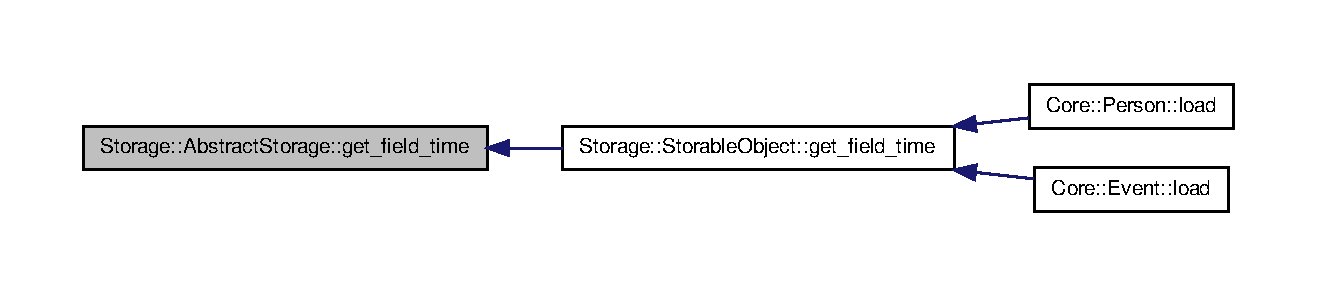
\includegraphics[width=400pt]{d6/da0/classStorage_1_1AbstractStorage_a87fe8d51934ab2403758d905ef313272_icgraph}
\end{center}
\end{figure}


\hypertarget{classStorage_1_1AbstractStorage_ae7c30697d68dc9d7de595388030d8e10}{
\index{Storage::AbstractStorage@{Storage::AbstractStorage}!get\_\-field\_\-vector@{get\_\-field\_\-vector}}
\index{get\_\-field\_\-vector@{get\_\-field\_\-vector}!Storage::AbstractStorage@{Storage::AbstractStorage}}
\subsubsection[{get\_\-field\_\-vector}]{\setlength{\rightskip}{0pt plus 5cm}virtual const std::vector$<${\bf StorableObject} $\ast$$>$ Storage::AbstractStorage::get\_\-field\_\-vector (
\begin{DoxyParamCaption}
\item[{const int}]{id, }
\item[{const std::string}]{field}
\end{DoxyParamCaption}
) const  throw (std::bad\_\-cast)\hspace{0.3cm}{\ttfamily  \mbox{[}protected, pure virtual\mbox{]}}}}
\label{d6/da0/classStorage_1_1AbstractStorage_ae7c30697d68dc9d7de595388030d8e10}


Return vector value of requested field. 


\begin{DoxyParams}[1]{Parameters}
\mbox{\tt in}  & {\em id} & Object identificator. \\
\hline
\mbox{\tt in}  & {\em field} & Field name. \\
\hline
\end{DoxyParams}
\begin{DoxyReturn}{Returns}
requested value.
\end{DoxyReturn}
This method must be realized in inherited classes. Throw an std::bad\_\-cast exception if requested field does not exists or keeped in another type. 

Implemented in \hyperlink{classSQLiteStorage_a818cc8edbbe849eabacbdc055a32ad6a}{SQLiteStorage}, and \hyperlink{classDummyStorage_afe36af3f3147027ebb6447192201c790}{DummyStorage}.



Here is the caller graph for this function:
\nopagebreak
\begin{figure}[H]
\begin{center}
\leavevmode
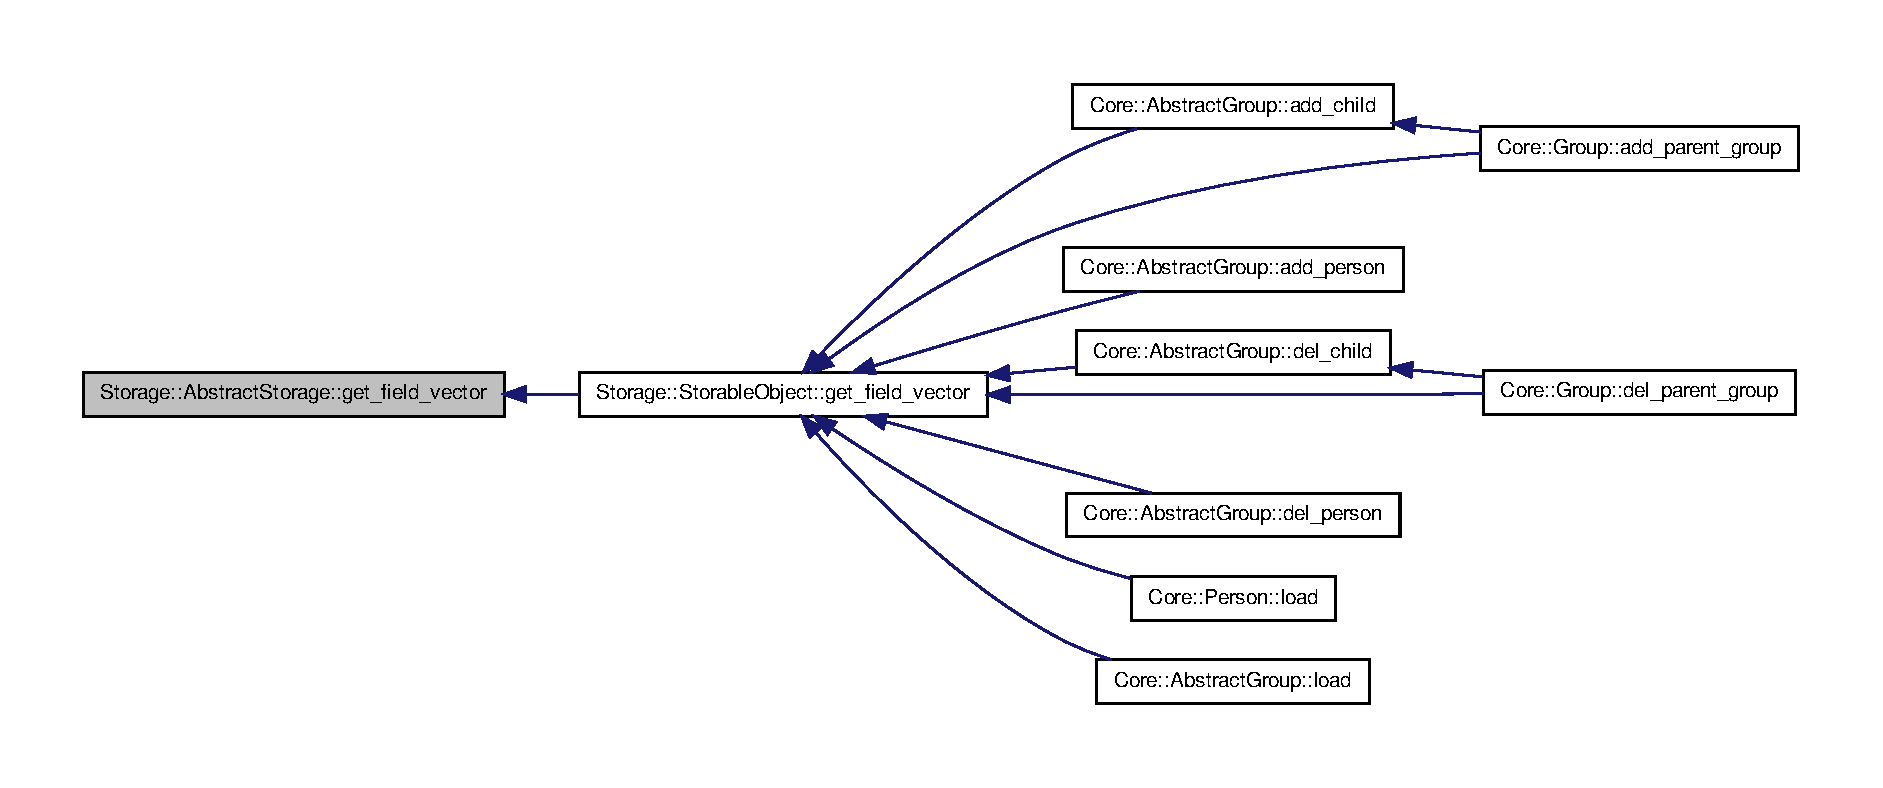
\includegraphics[width=400pt]{d6/da0/classStorage_1_1AbstractStorage_ae7c30697d68dc9d7de595388030d8e10_icgraph}
\end{center}
\end{figure}


\hypertarget{classStorage_1_1AbstractStorage_ab9e323067a58b74a7d1c835f0d1832c8}{
\index{Storage::AbstractStorage@{Storage::AbstractStorage}!new\_\-id@{new\_\-id}}
\index{new\_\-id@{new\_\-id}!Storage::AbstractStorage@{Storage::AbstractStorage}}
\subsubsection[{new\_\-id}]{\setlength{\rightskip}{0pt plus 5cm}const int AbstractStorage::new\_\-id (
\begin{DoxyParamCaption}
{}
\end{DoxyParamCaption}
)\hspace{0.3cm}{\ttfamily  \mbox{[}protected, virtual\mbox{]}}}}
\label{d6/da0/classStorage_1_1AbstractStorage_ab9e323067a58b74a7d1c835f0d1832c8}


Return new object identificator and reserve cell for it in the objects vector. 

\begin{DoxyReturn}{Returns}
New id.
\end{DoxyReturn}
You can redefine this method if you want to keep objects in other order.

Do not use this method anywhere, it used by create method. 

Here is the caller graph for this function:
\nopagebreak
\begin{figure}[H]
\begin{center}
\leavevmode
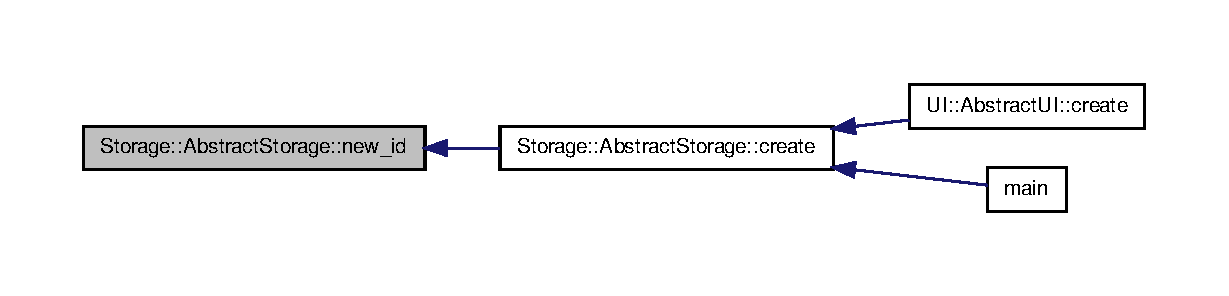
\includegraphics[width=400pt]{d6/da0/classStorage_1_1AbstractStorage_ab9e323067a58b74a7d1c835f0d1832c8_icgraph}
\end{center}
\end{figure}


\hypertarget{classStorage_1_1AbstractStorage_a21ff57c954664abb78d1d658a1da7afa}{
\index{Storage::AbstractStorage@{Storage::AbstractStorage}!object@{object}}
\index{object@{object}!Storage::AbstractStorage@{Storage::AbstractStorage}}
\subsubsection[{object}]{\setlength{\rightskip}{0pt plus 5cm}virtual {\bf StorableObject}$\ast$ Storage::AbstractStorage::object (
\begin{DoxyParamCaption}
\item[{const int}]{id}
\end{DoxyParamCaption}
) const  throw (std::bad\_\-cast)\hspace{0.3cm}{\ttfamily  \mbox{[}inline, virtual\mbox{]}}}}
\label{d6/da0/classStorage_1_1AbstractStorage_a21ff57c954664abb78d1d658a1da7afa}


Return object by id. 


\begin{DoxyParams}[1]{Parameters}
\mbox{\tt in}  & {\em id} & Object identificator. \\
\hline
\end{DoxyParams}
\begin{DoxyReturn}{Returns}
Requested object.
\end{DoxyReturn}
Use this method carefully. It can be moved to the protected or private on future. 

Here is the caller graph for this function:
\nopagebreak
\begin{figure}[H]
\begin{center}
\leavevmode
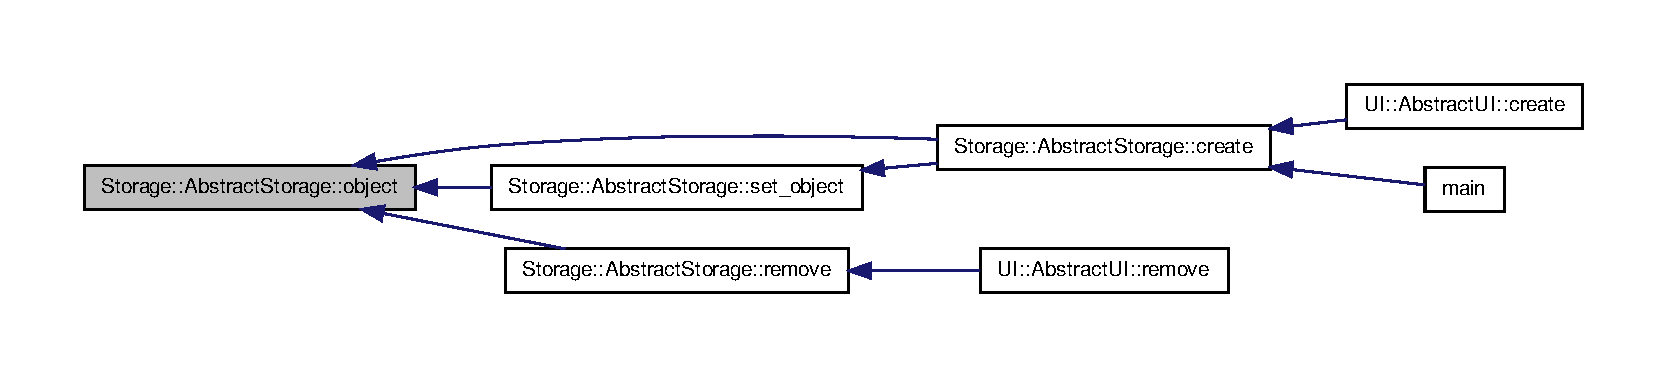
\includegraphics[width=400pt]{d6/da0/classStorage_1_1AbstractStorage_a21ff57c954664abb78d1d658a1da7afa_icgraph}
\end{center}
\end{figure}


\hypertarget{classStorage_1_1AbstractStorage_a5d114117d4954e01fd650251b829fdbf}{
\index{Storage::AbstractStorage@{Storage::AbstractStorage}!remove@{remove}}
\index{remove@{remove}!Storage::AbstractStorage@{Storage::AbstractStorage}}
\subsubsection[{remove}]{\setlength{\rightskip}{0pt plus 5cm}void AbstractStorage::remove (
\begin{DoxyParamCaption}
\item[{{\bf StorableObject} $\ast$}]{object}
\end{DoxyParamCaption}
)\hspace{0.3cm}{\ttfamily  \mbox{[}virtual\mbox{]}}}}
\label{d6/da0/classStorage_1_1AbstractStorage_a5d114117d4954e01fd650251b829fdbf}


Remove object from the storage. 


\begin{DoxyParams}[1]{Parameters}
\mbox{\tt in}  & {\em object} & Object to delete.\\
\hline
\end{DoxyParams}
You can redefine this method if you want to store objects in the other order. 

Here is the call graph for this function:
\nopagebreak
\begin{figure}[H]
\begin{center}
\leavevmode
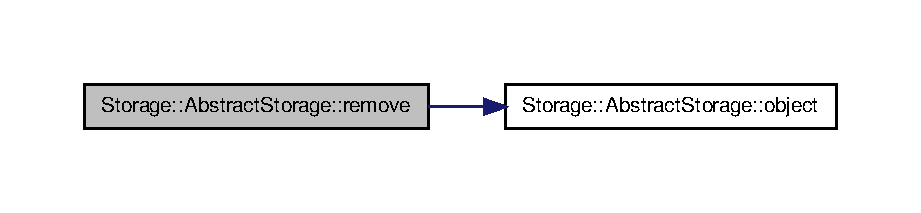
\includegraphics[width=400pt]{d6/da0/classStorage_1_1AbstractStorage_a5d114117d4954e01fd650251b829fdbf_cgraph}
\end{center}
\end{figure}




Here is the caller graph for this function:
\nopagebreak
\begin{figure}[H]
\begin{center}
\leavevmode
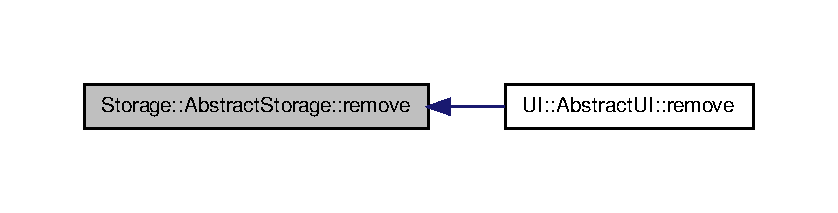
\includegraphics[width=400pt]{d6/da0/classStorage_1_1AbstractStorage_a5d114117d4954e01fd650251b829fdbf_icgraph}
\end{center}
\end{figure}


\hypertarget{classStorage_1_1AbstractStorage_a9304eea8cd6fffd77b1ccd26f85a061c}{
\index{Storage::AbstractStorage@{Storage::AbstractStorage}!search@{search}}
\index{search@{search}!Storage::AbstractStorage@{Storage::AbstractStorage}}
\subsubsection[{search}]{\setlength{\rightskip}{0pt plus 5cm}virtual std::vector$<${\bf StorableObject} $\ast$$>$$\ast$ Storage::AbstractStorage::search (
\begin{DoxyParamCaption}
\item[{std::vector$<$ {\bf Argument} $\ast$ $>$ \&}]{parameters}
\end{DoxyParamCaption}
)\hspace{0.3cm}{\ttfamily  \mbox{[}pure virtual\mbox{]}}}}
\label{d6/da0/classStorage_1_1AbstractStorage_a9304eea8cd6fffd77b1ccd26f85a061c}


Search objects by some parameters. 


\begin{DoxyParams}[1]{Parameters}
\mbox{\tt in}  & {\em parameters} & Search parameters. \\
\hline
\end{DoxyParams}
\begin{DoxyReturn}{Returns}
Vector of found objects.
\end{DoxyReturn}
Parameters are connected by logical AND. If parameter have not got a name, search value by the any field of specified type. If value is empty that all objects will satisfied. 

Implemented in \hyperlink{classDummyStorage_adea6bbcbaacaea1a728f09602d7c8d1d}{DummyStorage}.



Here is the caller graph for this function:
\nopagebreak
\begin{figure}[H]
\begin{center}
\leavevmode
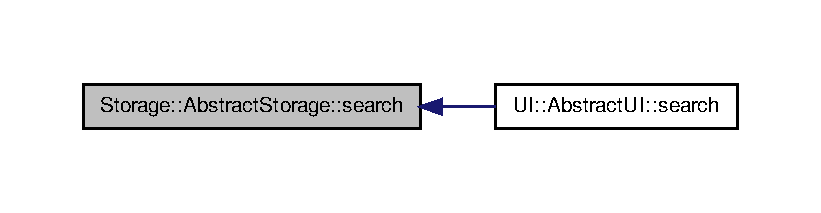
\includegraphics[width=394pt]{d6/da0/classStorage_1_1AbstractStorage_a9304eea8cd6fffd77b1ccd26f85a061c_icgraph}
\end{center}
\end{figure}


\hypertarget{classStorage_1_1AbstractStorage_ae5ee00e647f121b68ebada0f094058bc}{
\index{Storage::AbstractStorage@{Storage::AbstractStorage}!set\_\-field@{set\_\-field}}
\index{set\_\-field@{set\_\-field}!Storage::AbstractStorage@{Storage::AbstractStorage}}
\subsubsection[{set\_\-field}]{\setlength{\rightskip}{0pt plus 5cm}virtual void Storage::AbstractStorage::set\_\-field (
\begin{DoxyParamCaption}
\item[{const int}]{id, }
\item[{const std::string}]{field, }
\item[{const std::string}]{value}
\end{DoxyParamCaption}
)  throw (std::bad\_\-cast)\hspace{0.3cm}{\ttfamily  \mbox{[}protected, pure virtual\mbox{]}}}}
\label{d6/da0/classStorage_1_1AbstractStorage_ae5ee00e647f121b68ebada0f094058bc}


Set string value of requested field. 


\begin{DoxyParams}[1]{Parameters}
\mbox{\tt in}  & {\em id} & Object identificator. \\
\hline
\mbox{\tt in}  & {\em field} & Field name. \\
\hline
\mbox{\tt in}  & {\em value} & New value.\\
\hline
\end{DoxyParams}
This method must be realized in inherited classes. Throw an std::bad\_\-cast exception if requested field keeped in another type. 

Implemented in \hyperlink{classSQLiteStorage_ac353c289df54fce5f5658746824fcbac}{SQLiteStorage}, and \hyperlink{classDummyStorage_aaa0d3249ea3207fae78253b191b80854}{DummyStorage}.

\hypertarget{classStorage_1_1AbstractStorage_a7ef9f70b3fcbaa2863de2be695dc77c1}{
\index{Storage::AbstractStorage@{Storage::AbstractStorage}!set\_\-field@{set\_\-field}}
\index{set\_\-field@{set\_\-field}!Storage::AbstractStorage@{Storage::AbstractStorage}}
\subsubsection[{set\_\-field}]{\setlength{\rightskip}{0pt plus 5cm}virtual void Storage::AbstractStorage::set\_\-field (
\begin{DoxyParamCaption}
\item[{const int}]{id, }
\item[{const std::string}]{field, }
\item[{{\bf StorableObject} $\ast$}]{value}
\end{DoxyParamCaption}
)  throw (std::bad\_\-cast)\hspace{0.3cm}{\ttfamily  \mbox{[}protected, pure virtual\mbox{]}}}}
\label{d6/da0/classStorage_1_1AbstractStorage_a7ef9f70b3fcbaa2863de2be695dc77c1}


Set object value of requested field. 


\begin{DoxyParams}[1]{Parameters}
\mbox{\tt in}  & {\em id} & Object identificator. \\
\hline
\mbox{\tt in}  & {\em field} & Field name. \\
\hline
\mbox{\tt in}  & {\em value} & New value.\\
\hline
\end{DoxyParams}
This method must be realized in inherited classes. Throw an std::bad\_\-cast exception if requested field keeped in another type. 

Implemented in \hyperlink{classSQLiteStorage_ab2b3d9fcde8dbcd28eb66f60a6cf13ac}{SQLiteStorage}, and \hyperlink{classDummyStorage_ae2e39a3cee22fd90790a7528f0c7ad59}{DummyStorage}.

\hypertarget{classStorage_1_1AbstractStorage_a50ee4a829bc067a9291a11aa99ec0f16}{
\index{Storage::AbstractStorage@{Storage::AbstractStorage}!set\_\-field@{set\_\-field}}
\index{set\_\-field@{set\_\-field}!Storage::AbstractStorage@{Storage::AbstractStorage}}
\subsubsection[{set\_\-field}]{\setlength{\rightskip}{0pt plus 5cm}virtual void Storage::AbstractStorage::set\_\-field (
\begin{DoxyParamCaption}
\item[{const int}]{id, }
\item[{const std::string}]{field, }
\item[{const time\_\-t}]{value}
\end{DoxyParamCaption}
)  throw (std::bad\_\-cast)\hspace{0.3cm}{\ttfamily  \mbox{[}protected, pure virtual\mbox{]}}}}
\label{d6/da0/classStorage_1_1AbstractStorage_a50ee4a829bc067a9291a11aa99ec0f16}


Set time value of requested field. 


\begin{DoxyParams}[1]{Parameters}
\mbox{\tt in}  & {\em id} & Object identificator. \\
\hline
\mbox{\tt in}  & {\em field} & Field name. \\
\hline
\mbox{\tt in}  & {\em value} & New value.\\
\hline
\end{DoxyParams}
This method must be realized in inherited classes. Throw an std::bad\_\-cast exception if requested field keeped in another type. 

Implemented in \hyperlink{classSQLiteStorage_a36665e18b5290da4c7bab56d22703d03}{SQLiteStorage}, and \hyperlink{classDummyStorage_a51662a853e821fda1828e8756d58f1df}{DummyStorage}.

\hypertarget{classStorage_1_1AbstractStorage_acdd090d0beb6a8241914e7d78a7f2c0c}{
\index{Storage::AbstractStorage@{Storage::AbstractStorage}!set\_\-field@{set\_\-field}}
\index{set\_\-field@{set\_\-field}!Storage::AbstractStorage@{Storage::AbstractStorage}}
\subsubsection[{set\_\-field}]{\setlength{\rightskip}{0pt plus 5cm}virtual void Storage::AbstractStorage::set\_\-field (
\begin{DoxyParamCaption}
\item[{const int}]{id, }
\item[{const std::string}]{field, }
\item[{const int}]{value}
\end{DoxyParamCaption}
)  throw (std::bad\_\-cast)\hspace{0.3cm}{\ttfamily  \mbox{[}protected, pure virtual\mbox{]}}}}
\label{d6/da0/classStorage_1_1AbstractStorage_acdd090d0beb6a8241914e7d78a7f2c0c}


Set integer value of requested field. 


\begin{DoxyParams}[1]{Parameters}
\mbox{\tt in}  & {\em id} & Object identificator. \\
\hline
\mbox{\tt in}  & {\em field} & Field name. \\
\hline
\mbox{\tt in}  & {\em value} & New value.\\
\hline
\end{DoxyParams}
This method must be realized in inherited classes. Throw an std::bad\_\-cast exception if requested field keeped in another type. 

Implemented in \hyperlink{classSQLiteStorage_a3e1271c2699a0e5a82452a21e5d1af63}{SQLiteStorage}, and \hyperlink{classDummyStorage_ab22488d00b8969af5356bc344672bd18}{DummyStorage}.



Here is the caller graph for this function:
\nopagebreak
\begin{figure}[H]
\begin{center}
\leavevmode
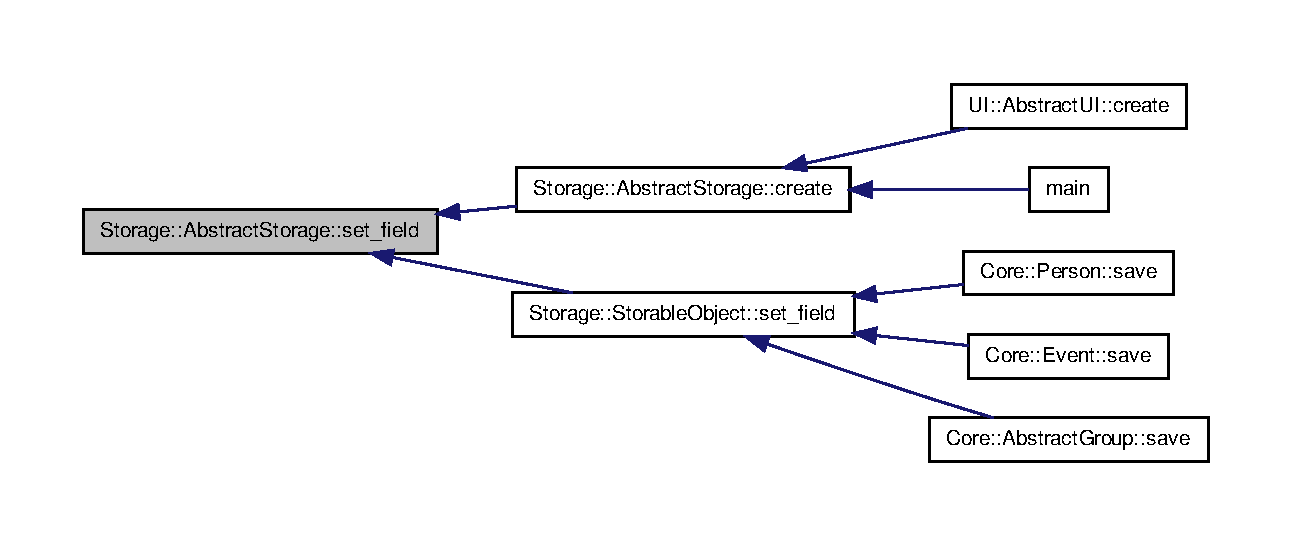
\includegraphics[width=400pt]{d6/da0/classStorage_1_1AbstractStorage_acdd090d0beb6a8241914e7d78a7f2c0c_icgraph}
\end{center}
\end{figure}


\hypertarget{classStorage_1_1AbstractStorage_a50925678c74c09acd8549a541fdbbe9f}{
\index{Storage::AbstractStorage@{Storage::AbstractStorage}!set\_\-field\_\-enum@{set\_\-field\_\-enum}}
\index{set\_\-field\_\-enum@{set\_\-field\_\-enum}!Storage::AbstractStorage@{Storage::AbstractStorage}}
\subsubsection[{set\_\-field\_\-enum}]{\setlength{\rightskip}{0pt plus 5cm}virtual void Storage::AbstractStorage::set\_\-field\_\-enum (
\begin{DoxyParamCaption}
\item[{const int}]{id, }
\item[{const std::string}]{field, }
\item[{const std::string}]{value}
\end{DoxyParamCaption}
)  throw (std::bad\_\-cast)\hspace{0.3cm}{\ttfamily  \mbox{[}protected, pure virtual\mbox{]}}}}
\label{d6/da0/classStorage_1_1AbstractStorage_a50925678c74c09acd8549a541fdbbe9f}


Set enum value of requested field. 


\begin{DoxyParams}[1]{Parameters}
\mbox{\tt in}  & {\em id} & Object identificator. \\
\hline
\mbox{\tt in}  & {\em field} & Field name. \\
\hline
\mbox{\tt in}  & {\em value} & New value.\\
\hline
\end{DoxyParams}
This method must be realized in inherited classes. Throw an std::bad\_\-cast exception if requested field keeped in another type. 

Implemented in \hyperlink{classSQLiteStorage_a1b8a3f2ad138447ad5815e857eea333e}{SQLiteStorage}, and \hyperlink{classDummyStorage_a0655a6f7c822adbe174d1c7fe7c9ea34}{DummyStorage}.



Here is the caller graph for this function:
\nopagebreak
\begin{figure}[H]
\begin{center}
\leavevmode
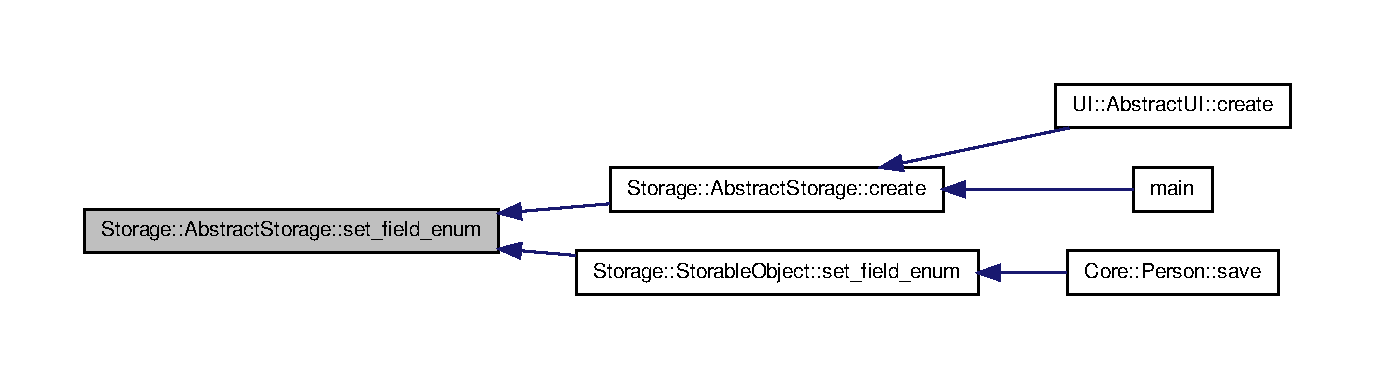
\includegraphics[width=400pt]{d6/da0/classStorage_1_1AbstractStorage_a50925678c74c09acd8549a541fdbbe9f_icgraph}
\end{center}
\end{figure}


\hypertarget{classStorage_1_1AbstractStorage_a24af03b9a68ace199b0a6fa812abad39}{
\index{Storage::AbstractStorage@{Storage::AbstractStorage}!set\_\-field\_\-vector@{set\_\-field\_\-vector}}
\index{set\_\-field\_\-vector@{set\_\-field\_\-vector}!Storage::AbstractStorage@{Storage::AbstractStorage}}
\subsubsection[{set\_\-field\_\-vector}]{\setlength{\rightskip}{0pt plus 5cm}virtual void Storage::AbstractStorage::set\_\-field\_\-vector (
\begin{DoxyParamCaption}
\item[{const int}]{id, }
\item[{const std::string}]{field, }
\item[{const std::vector$<$ {\bf StorableObject} $\ast$ $>$}]{vector}
\end{DoxyParamCaption}
)  throw (std::bad\_\-cast)\hspace{0.3cm}{\ttfamily  \mbox{[}protected, pure virtual\mbox{]}}}}
\label{d6/da0/classStorage_1_1AbstractStorage_a24af03b9a68ace199b0a6fa812abad39}


Set vector value of requested field. 


\begin{DoxyParams}[1]{Parameters}
\mbox{\tt in}  & {\em id} & Object identificator. \\
\hline
\mbox{\tt in}  & {\em field} & Field name.  \mbox{[}in\mbox{]} value New value.\\
\hline
\end{DoxyParams}
This method must be realized in inherited classes. Throw an std::bad\_\-cast exception if requested field keeped in another type. 

Implemented in \hyperlink{classSQLiteStorage_a41c576c779146896a0cd0b18228a643e}{SQLiteStorage}, and \hyperlink{classDummyStorage_a6102ef89119b0ee1525439b3fd7043ce}{DummyStorage}.



Here is the caller graph for this function:
\nopagebreak
\begin{figure}[H]
\begin{center}
\leavevmode
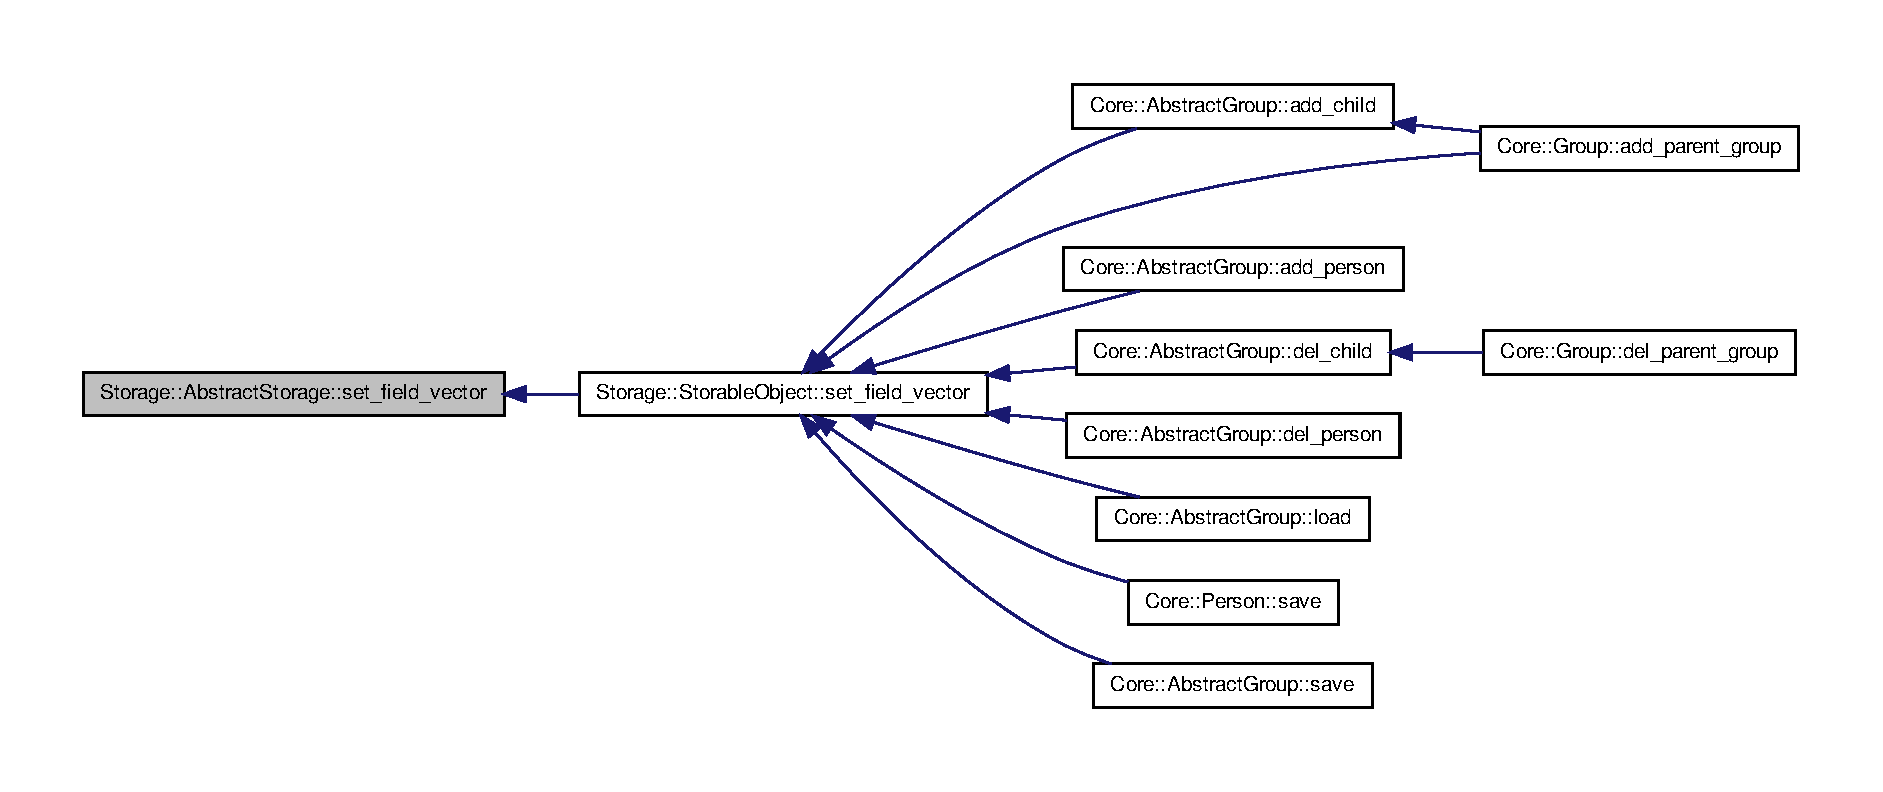
\includegraphics[width=400pt]{d6/da0/classStorage_1_1AbstractStorage_a24af03b9a68ace199b0a6fa812abad39_icgraph}
\end{center}
\end{figure}


\hypertarget{classStorage_1_1AbstractStorage_a641a6b75fe34c51943902d846ff66328}{
\index{Storage::AbstractStorage@{Storage::AbstractStorage}!set\_\-object@{set\_\-object}}
\index{set\_\-object@{set\_\-object}!Storage::AbstractStorage@{Storage::AbstractStorage}}
\subsubsection[{set\_\-object}]{\setlength{\rightskip}{0pt plus 5cm}void AbstractStorage::set\_\-object (
\begin{DoxyParamCaption}
\item[{{\bf StorableObject} $\ast$}]{object}
\end{DoxyParamCaption}
)\hspace{0.3cm}{\ttfamily  \mbox{[}protected, virtual\mbox{]}}}}
\label{d6/da0/classStorage_1_1AbstractStorage_a641a6b75fe34c51943902d846ff66328}


Set integer value of requested field. 


\begin{DoxyParams}[1]{Parameters}
\mbox{\tt in}  & {\em Object} & to save.\\
\hline
\end{DoxyParams}
You can redefine this method if you want to keep objects in other order.

Do not use this method anywhere, it used by create method. 

Here is the call graph for this function:
\nopagebreak
\begin{figure}[H]
\begin{center}
\leavevmode
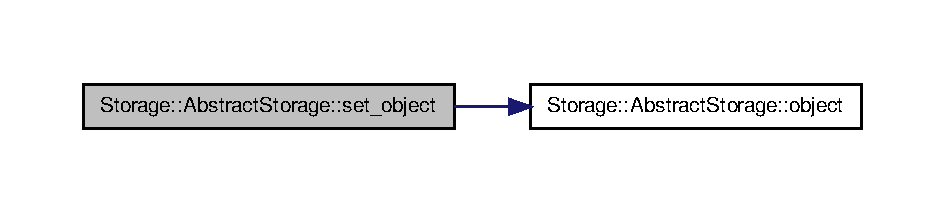
\includegraphics[width=400pt]{d6/da0/classStorage_1_1AbstractStorage_a641a6b75fe34c51943902d846ff66328_cgraph}
\end{center}
\end{figure}




Here is the caller graph for this function:
\nopagebreak
\begin{figure}[H]
\begin{center}
\leavevmode
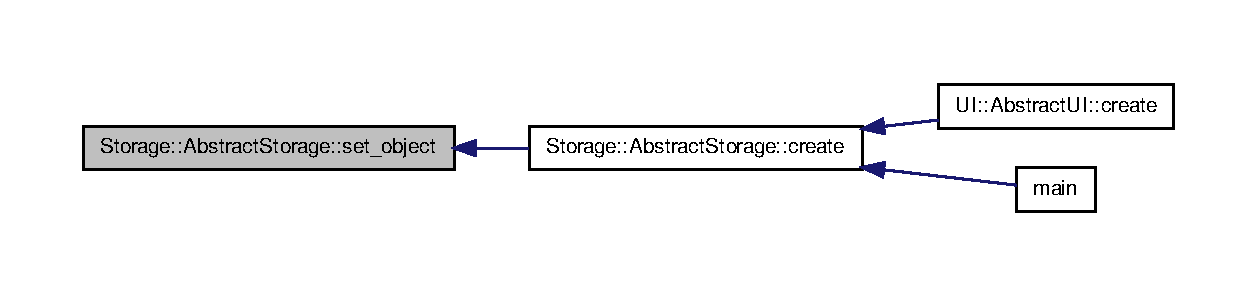
\includegraphics[width=400pt]{d6/da0/classStorage_1_1AbstractStorage_a641a6b75fe34c51943902d846ff66328_icgraph}
\end{center}
\end{figure}




\subsection{Friends And Related Function Documentation}
\hypertarget{classStorage_1_1AbstractStorage_ac344c900799ce1069f4324f043f17763}{
\index{Storage::AbstractStorage@{Storage::AbstractStorage}!StorableObject@{StorableObject}}
\index{StorableObject@{StorableObject}!Storage::AbstractStorage@{Storage::AbstractStorage}}
\subsubsection[{StorableObject}]{\setlength{\rightskip}{0pt plus 5cm}friend class {\bf StorableObject}\hspace{0.3cm}{\ttfamily  \mbox{[}friend\mbox{]}}}}
\label{d6/da0/classStorage_1_1AbstractStorage_ac344c900799ce1069f4324f043f17763}


\subsection{Member Data Documentation}
\hypertarget{classStorage_1_1AbstractStorage_a54758736009f559baf85a2d477b4d370}{
\index{Storage::AbstractStorage@{Storage::AbstractStorage}!objects\_\-@{objects\_\-}}
\index{objects\_\-@{objects\_\-}!Storage::AbstractStorage@{Storage::AbstractStorage}}
\subsubsection[{objects\_\-}]{\setlength{\rightskip}{0pt plus 5cm}std::vector$<${\bf StorableObject} $\ast$$>$ {\bf Storage::AbstractStorage::objects\_\-}\hspace{0.3cm}{\ttfamily  \mbox{[}protected\mbox{]}}}}
\label{d6/da0/classStorage_1_1AbstractStorage_a54758736009f559baf85a2d477b4d370}
Model objects. Each object must be saved here for correct work of storage.

You must use this only with \hyperlink{classStorage_1_1AbstractStorage_a21ff57c954664abb78d1d658a1da7afa}{object()}, set\_\-object and \hyperlink{classStorage_1_1AbstractStorage_ab9e323067a58b74a7d1c835f0d1832c8}{new\_\-id()} mehods, you can redefine this methods but do not use this field in other code. 

The documentation for this class was generated from the following files:\begin{DoxyCompactItemize}
\item 
src/include/\hyperlink{abstractstorage_8h}{abstractstorage.h}\item 
src/storage/\hyperlink{abstractstorage_8cpp}{abstractstorage.cpp}\end{DoxyCompactItemize}

\hypertarget{classUI_1_1AbstractUI}{
\section{UI::AbstractUI Class Reference}
\label{de/dda/classUI_1_1AbstractUI}\index{UI::AbstractUI@{UI::AbstractUI}}
}


{\ttfamily \#include $<$abstractui.h$>$}

\subsection*{Public Member Functions}
\begin{DoxyCompactItemize}
\item 
\hyperlink{classUI_1_1AbstractUI_a35092e69be8cc4406582540286db5a69}{AbstractUI} (\hyperlink{classStorage_1_1AbstractStorage}{Storage::AbstractStorage} \&storage)
\end{DoxyCompactItemize}
\subsection*{Protected Member Functions}
\begin{DoxyCompactItemize}
\item 
std::vector$<$ \hyperlink{classUI_1_1UsersObject}{UsersObject} $\ast$ $>$ \& \hyperlink{classUI_1_1AbstractUI_ab09dc4b586d429a5238d1b09c98d2a4b}{cache} ()
\item 
void \hyperlink{classUI_1_1AbstractUI_aaa55abbdeb863b8189393e929f643335}{search} (std::vector$<$ \hyperlink{structStorage_1_1AbstractStorage_1_1Argument}{Storage::AbstractStorage::Argument} $\ast$ $>$ \&parameters)
\item 
{\footnotesize template$<$class T $>$ }\\void \hyperlink{classUI_1_1AbstractUI_a485b7a347d6b07f6dc44a3174cb96eaa}{create} (const std::vector$<$ const \hyperlink{structStorage_1_1AbstractStorage_1_1Argument}{Storage::AbstractStorage::Argument} $>$ \&parameters)
\item 
void \hyperlink{classUI_1_1AbstractUI_a160bde97ba2106267a8850db226d9790}{remove} (\hyperlink{classUI_1_1UsersObject}{UsersObject} $\ast$object)
\end{DoxyCompactItemize}


\subsection{Constructor \& Destructor Documentation}
\hypertarget{classUI_1_1AbstractUI_a35092e69be8cc4406582540286db5a69}{
\index{UI::AbstractUI@{UI::AbstractUI}!AbstractUI@{AbstractUI}}
\index{AbstractUI@{AbstractUI}!UI::AbstractUI@{UI::AbstractUI}}
\subsubsection[{AbstractUI}]{\setlength{\rightskip}{0pt plus 5cm}UI::AbstractUI::AbstractUI (
\begin{DoxyParamCaption}
\item[{{\bf Storage::AbstractStorage} \&}]{storage}
\end{DoxyParamCaption}
)\hspace{0.3cm}{\ttfamily  \mbox{[}inline\mbox{]}}}}
\label{de/dda/classUI_1_1AbstractUI_a35092e69be8cc4406582540286db5a69}


\subsection{Member Function Documentation}
\hypertarget{classUI_1_1AbstractUI_ab09dc4b586d429a5238d1b09c98d2a4b}{
\index{UI::AbstractUI@{UI::AbstractUI}!cache@{cache}}
\index{cache@{cache}!UI::AbstractUI@{UI::AbstractUI}}
\subsubsection[{cache}]{\setlength{\rightskip}{0pt plus 5cm}std::vector$<${\bf UsersObject} $\ast$$>$\& UI::AbstractUI::cache (
\begin{DoxyParamCaption}
{}
\end{DoxyParamCaption}
)\hspace{0.3cm}{\ttfamily  \mbox{[}inline, protected\mbox{]}}}}
\label{de/dda/classUI_1_1AbstractUI_ab09dc4b586d429a5238d1b09c98d2a4b}
\hypertarget{classUI_1_1AbstractUI_a485b7a347d6b07f6dc44a3174cb96eaa}{
\index{UI::AbstractUI@{UI::AbstractUI}!create@{create}}
\index{create@{create}!UI::AbstractUI@{UI::AbstractUI}}
\subsubsection[{create}]{\setlength{\rightskip}{0pt plus 5cm}template$<$class T $>$ void AbstractUI::create (
\begin{DoxyParamCaption}
\item[{const std::vector$<$ const {\bf Storage::AbstractStorage::Argument} $>$ \&}]{parameters}
\end{DoxyParamCaption}
)\hspace{0.3cm}{\ttfamily  \mbox{[}protected\mbox{]}}}}
\label{de/dda/classUI_1_1AbstractUI_a485b7a347d6b07f6dc44a3174cb96eaa}
\hypertarget{classUI_1_1AbstractUI_a160bde97ba2106267a8850db226d9790}{
\index{UI::AbstractUI@{UI::AbstractUI}!remove@{remove}}
\index{remove@{remove}!UI::AbstractUI@{UI::AbstractUI}}
\subsubsection[{remove}]{\setlength{\rightskip}{0pt plus 5cm}void AbstractUI::remove (
\begin{DoxyParamCaption}
\item[{{\bf UsersObject} $\ast$}]{object}
\end{DoxyParamCaption}
)\hspace{0.3cm}{\ttfamily  \mbox{[}protected\mbox{]}}}}
\label{de/dda/classUI_1_1AbstractUI_a160bde97ba2106267a8850db226d9790}
\hypertarget{classUI_1_1AbstractUI_aaa55abbdeb863b8189393e929f643335}{
\index{UI::AbstractUI@{UI::AbstractUI}!search@{search}}
\index{search@{search}!UI::AbstractUI@{UI::AbstractUI}}
\subsubsection[{search}]{\setlength{\rightskip}{0pt plus 5cm}void AbstractUI::search (
\begin{DoxyParamCaption}
\item[{std::vector$<$ {\bf Storage::AbstractStorage::Argument} $\ast$ $>$ \&}]{parameters}
\end{DoxyParamCaption}
)\hspace{0.3cm}{\ttfamily  \mbox{[}protected\mbox{]}}}}
\label{de/dda/classUI_1_1AbstractUI_aaa55abbdeb863b8189393e929f643335}


The documentation for this class was generated from the following files:\begin{DoxyCompactItemize}
\item 
src/include/\hyperlink{abstractui_8h}{abstractui.h}\item 
src/ui/\hyperlink{abstractui_8cpp}{abstractui.cpp}\end{DoxyCompactItemize}

\hypertarget{structStorage_1_1AbstractStorage_1_1Argument}{
\section{Storage::AbstractStorage::Argument Struct Reference}
\label{d9/dc9/structStorage_1_1AbstractStorage_1_1Argument}\index{Storage::AbstractStorage::Argument@{Storage::AbstractStorage::Argument}}
}


{\ttfamily \#include $<$abstractstorage.h$>$}

\subsection*{Public Types}
\begin{DoxyCompactItemize}
\item 
enum \{ \hyperlink{structStorage_1_1AbstractStorage_1_1Argument_a92adab5cf7e02947e2e75fba5e11446ca3268a68276a4ac73701de323858c945b}{STRING}, 
\hyperlink{structStorage_1_1AbstractStorage_1_1Argument_a92adab5cf7e02947e2e75fba5e11446ca4f57d3a5ac601598730fb58b08c81540}{INTEGER}, 
\hyperlink{structStorage_1_1AbstractStorage_1_1Argument_a92adab5cf7e02947e2e75fba5e11446ca6f9cbb024f036014248e8322253da11e}{TIME}, 
\hyperlink{structStorage_1_1AbstractStorage_1_1Argument_a92adab5cf7e02947e2e75fba5e11446ca37240303f27a558e24e9e07d1abfa215}{ENUMERATION}
 \}
\end{DoxyCompactItemize}
\subsection*{Public Attributes}
\begin{DoxyCompactItemize}
\item 
const std::string \hyperlink{structStorage_1_1AbstractStorage_1_1Argument_ad48a91372dd1a9445b4ddcee0bc8336a}{field}
\item 
enum Storage::AbstractStorage::Argument:: \{ ... \}  \hyperlink{structStorage_1_1AbstractStorage_1_1Argument_a77f04e835f26305c4222df78c07f8efd}{type}
\item 
const std::string \hyperlink{structStorage_1_1AbstractStorage_1_1Argument_ab8ea8281cdefeb901a267261ed2e0478}{string}
\item 
const int \hyperlink{structStorage_1_1AbstractStorage_1_1Argument_a6b20329db4720c44c45d8380f840dbec}{integer}
\item 
const time\_\-t \hyperlink{structStorage_1_1AbstractStorage_1_1Argument_ae6cc69656647a6cccf725a0156373a51}{time}
\end{DoxyCompactItemize}


\subsection{Member Enumeration Documentation}
\hypertarget{structStorage_1_1AbstractStorage_1_1Argument_a92adab5cf7e02947e2e75fba5e11446c}{
\subsubsection[{"@0}]{\setlength{\rightskip}{0pt plus 5cm}anonymous enum}}
\label{d9/dc9/structStorage_1_1AbstractStorage_1_1Argument_a92adab5cf7e02947e2e75fba5e11446c}
\begin{Desc}
\item[Enumerator: ]\par
\begin{description}
\index{STRING@{STRING}!Storage::AbstractStorage::Argument@{Storage::AbstractStorage::Argument}}\index{Storage::AbstractStorage::Argument@{Storage::AbstractStorage::Argument}!STRING@{STRING}}\item[{\em 
\hypertarget{structStorage_1_1AbstractStorage_1_1Argument_a92adab5cf7e02947e2e75fba5e11446ca3268a68276a4ac73701de323858c945b}{
STRING}
\label{d9/dc9/structStorage_1_1AbstractStorage_1_1Argument_a92adab5cf7e02947e2e75fba5e11446ca3268a68276a4ac73701de323858c945b}
}]\index{INTEGER@{INTEGER}!Storage::AbstractStorage::Argument@{Storage::AbstractStorage::Argument}}\index{Storage::AbstractStorage::Argument@{Storage::AbstractStorage::Argument}!INTEGER@{INTEGER}}\item[{\em 
\hypertarget{structStorage_1_1AbstractStorage_1_1Argument_a92adab5cf7e02947e2e75fba5e11446ca4f57d3a5ac601598730fb58b08c81540}{
INTEGER}
\label{d9/dc9/structStorage_1_1AbstractStorage_1_1Argument_a92adab5cf7e02947e2e75fba5e11446ca4f57d3a5ac601598730fb58b08c81540}
}]\index{TIME@{TIME}!Storage::AbstractStorage::Argument@{Storage::AbstractStorage::Argument}}\index{Storage::AbstractStorage::Argument@{Storage::AbstractStorage::Argument}!TIME@{TIME}}\item[{\em 
\hypertarget{structStorage_1_1AbstractStorage_1_1Argument_a92adab5cf7e02947e2e75fba5e11446ca6f9cbb024f036014248e8322253da11e}{
TIME}
\label{d9/dc9/structStorage_1_1AbstractStorage_1_1Argument_a92adab5cf7e02947e2e75fba5e11446ca6f9cbb024f036014248e8322253da11e}
}]\index{ENUMERATION@{ENUMERATION}!Storage::AbstractStorage::Argument@{Storage::AbstractStorage::Argument}}\index{Storage::AbstractStorage::Argument@{Storage::AbstractStorage::Argument}!ENUMERATION@{ENUMERATION}}\item[{\em 
\hypertarget{structStorage_1_1AbstractStorage_1_1Argument_a92adab5cf7e02947e2e75fba5e11446ca37240303f27a558e24e9e07d1abfa215}{
ENUMERATION}
\label{d9/dc9/structStorage_1_1AbstractStorage_1_1Argument_a92adab5cf7e02947e2e75fba5e11446ca37240303f27a558e24e9e07d1abfa215}
}]\end{description}
\end{Desc}



\subsection{Member Data Documentation}
\hypertarget{structStorage_1_1AbstractStorage_1_1Argument_ad48a91372dd1a9445b4ddcee0bc8336a}{
\index{Storage::AbstractStorage::Argument@{Storage::AbstractStorage::Argument}!field@{field}}
\index{field@{field}!Storage::AbstractStorage::Argument@{Storage::AbstractStorage::Argument}}
\subsubsection[{field}]{\setlength{\rightskip}{0pt plus 5cm}const std::string {\bf Storage::AbstractStorage::Argument::field}}}
\label{d9/dc9/structStorage_1_1AbstractStorage_1_1Argument_ad48a91372dd1a9445b4ddcee0bc8336a}
\hypertarget{structStorage_1_1AbstractStorage_1_1Argument_a6b20329db4720c44c45d8380f840dbec}{
\index{Storage::AbstractStorage::Argument@{Storage::AbstractStorage::Argument}!integer@{integer}}
\index{integer@{integer}!Storage::AbstractStorage::Argument@{Storage::AbstractStorage::Argument}}
\subsubsection[{integer}]{\setlength{\rightskip}{0pt plus 5cm}const int {\bf Storage::AbstractStorage::Argument::integer}}}
\label{d9/dc9/structStorage_1_1AbstractStorage_1_1Argument_a6b20329db4720c44c45d8380f840dbec}
\hypertarget{structStorage_1_1AbstractStorage_1_1Argument_ab8ea8281cdefeb901a267261ed2e0478}{
\index{Storage::AbstractStorage::Argument@{Storage::AbstractStorage::Argument}!string@{string}}
\index{string@{string}!Storage::AbstractStorage::Argument@{Storage::AbstractStorage::Argument}}
\subsubsection[{string}]{\setlength{\rightskip}{0pt plus 5cm}const std::string {\bf Storage::AbstractStorage::Argument::string}}}
\label{d9/dc9/structStorage_1_1AbstractStorage_1_1Argument_ab8ea8281cdefeb901a267261ed2e0478}
\hypertarget{structStorage_1_1AbstractStorage_1_1Argument_ae6cc69656647a6cccf725a0156373a51}{
\index{Storage::AbstractStorage::Argument@{Storage::AbstractStorage::Argument}!time@{time}}
\index{time@{time}!Storage::AbstractStorage::Argument@{Storage::AbstractStorage::Argument}}
\subsubsection[{time}]{\setlength{\rightskip}{0pt plus 5cm}const time\_\-t {\bf Storage::AbstractStorage::Argument::time}}}
\label{d9/dc9/structStorage_1_1AbstractStorage_1_1Argument_ae6cc69656647a6cccf725a0156373a51}
\hypertarget{structStorage_1_1AbstractStorage_1_1Argument_a77f04e835f26305c4222df78c07f8efd}{
\index{Storage::AbstractStorage::Argument@{Storage::AbstractStorage::Argument}!type@{type}}
\index{type@{type}!Storage::AbstractStorage::Argument@{Storage::AbstractStorage::Argument}}
\subsubsection[{type}]{\setlength{\rightskip}{0pt plus 5cm}enum \{ ... \}   {\bf Storage::AbstractStorage::Argument::type}}}
\label{d9/dc9/structStorage_1_1AbstractStorage_1_1Argument_a77f04e835f26305c4222df78c07f8efd}


The documentation for this struct was generated from the following file:\begin{DoxyCompactItemize}
\item 
src/include/\hyperlink{abstractstorage_8h}{abstractstorage.h}\end{DoxyCompactItemize}

\hypertarget{classDummyStorage}{
\section{DummyStorage Class Reference}
\label{d0/df2/classDummyStorage}\index{DummyStorage@{DummyStorage}}
}
Inheritance diagram for DummyStorage:\begin{figure}[H]
\begin{center}
\leavevmode
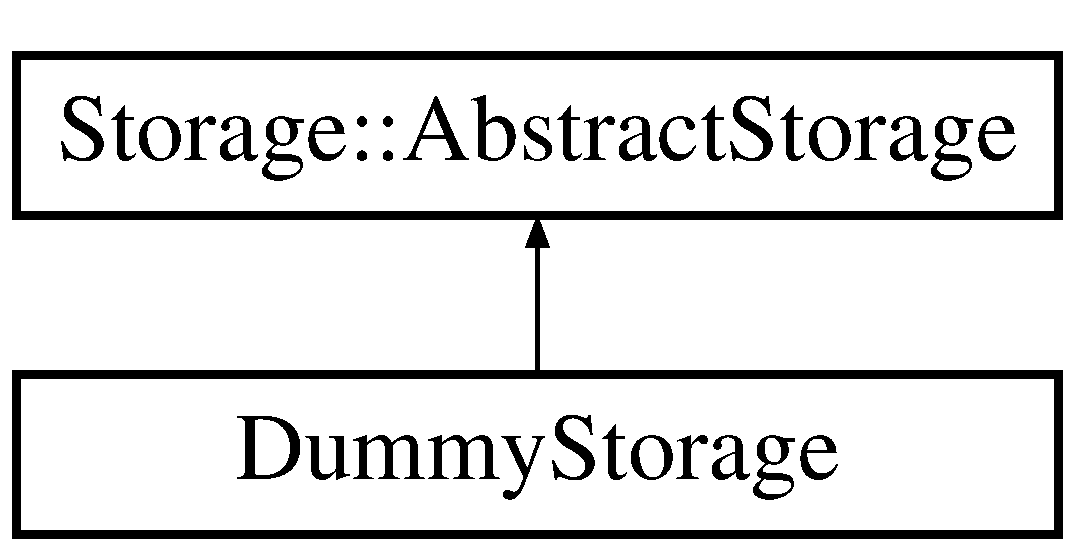
\includegraphics[height=2.000000cm]{d0/df2/classDummyStorage}
\end{center}
\end{figure}
\subsection*{Public Member Functions}
\begin{DoxyCompactItemize}
\item 
virtual std::vector$<$ \hyperlink{classStorage_1_1StorableObject}{Storage::StorableObject} $\ast$ $>$ $\ast$ \hyperlink{classDummyStorage_adea6bbcbaacaea1a728f09602d7c8d1d}{search} (std::vector$<$ \hyperlink{structStorage_1_1AbstractStorage_1_1Argument}{Argument} $\ast$ $>$ \&)
\begin{DoxyCompactList}\small\item\em Search objects by some parameters. \item\end{DoxyCompactList}\end{DoxyCompactItemize}
\subsection*{Protected Member Functions}
\begin{DoxyCompactItemize}
\item 
virtual const int \hyperlink{classDummyStorage_a275263eba82a652005292f01a120af8e}{get\_\-field\_\-int} (const int id, const std::string name) const   throw (std::bad\_\-cast)
\begin{DoxyCompactList}\small\item\em Return integer value of requested field. \item\end{DoxyCompactList}\item 
virtual const std::string \hyperlink{classDummyStorage_a410ef9d239193e25f830c49140e18293}{get\_\-field\_\-string} (const int id, const std::string name) const   throw (std::bad\_\-cast)
\begin{DoxyCompactList}\small\item\em Return string value of requested field. \item\end{DoxyCompactList}\item 
virtual const time\_\-t \hyperlink{classDummyStorage_a978ef9d688175e3739bb478f4c9b5313}{get\_\-field\_\-time} (const int id, const std::string name) const   throw (std::bad\_\-cast)
\begin{DoxyCompactList}\small\item\em Return time value of requested field. \item\end{DoxyCompactList}\item 
virtual const std::string \hyperlink{classDummyStorage_a1101739c23fbf79b009558553180ef1a}{get\_\-field\_\-enum} (const int id, const std::string name) const   throw (std::bad\_\-cast)
\begin{DoxyCompactList}\small\item\em Return enum value of requested field. \item\end{DoxyCompactList}\item 
virtual \hyperlink{classStorage_1_1StorableObject}{Storage::StorableObject} $\ast$ \hyperlink{classDummyStorage_a7135d171d9b83c2fbf72851fa9ea852a}{get\_\-field\_\-object} (const int id, const std::string name) const   throw (std::bad\_\-cast)
\begin{DoxyCompactList}\small\item\em Return object value of requested field. \item\end{DoxyCompactList}\item 
virtual const std::vector$<$ \hyperlink{classStorage_1_1StorableObject}{Storage::StorableObject} $\ast$ $>$ \hyperlink{classDummyStorage_afe36af3f3147027ebb6447192201c790}{get\_\-field\_\-vector} (const int id, const std::string name) const   throw (std::bad\_\-cast)
\begin{DoxyCompactList}\small\item\em Return vector value of requested field. \item\end{DoxyCompactList}\item 
virtual void \hyperlink{classDummyStorage_ab22488d00b8969af5356bc344672bd18}{set\_\-field} (const int id, const std::string name, const int value)  throw (std::bad\_\-cast)
\begin{DoxyCompactList}\small\item\em Set integer value of requested field. \item\end{DoxyCompactList}\item 
virtual void \hyperlink{classDummyStorage_aaa0d3249ea3207fae78253b191b80854}{set\_\-field} (const int id, const std::string name, const std::string value)  throw (std::bad\_\-cast)
\begin{DoxyCompactList}\small\item\em Set string value of requested field. \item\end{DoxyCompactList}\item 
virtual void \hyperlink{classDummyStorage_a51662a853e821fda1828e8756d58f1df}{set\_\-field} (const int id, const std::string name, const time\_\-t value)  throw (std::bad\_\-cast)
\begin{DoxyCompactList}\small\item\em Set time value of requested field. \item\end{DoxyCompactList}\item 
virtual void \hyperlink{classDummyStorage_a0655a6f7c822adbe174d1c7fe7c9ea34}{set\_\-field\_\-enum} (const int id, const std::string name, const std::string value)  throw (std::bad\_\-cast)
\begin{DoxyCompactList}\small\item\em Set enum value of requested field. \item\end{DoxyCompactList}\item 
virtual void \hyperlink{classDummyStorage_ae2e39a3cee22fd90790a7528f0c7ad59}{set\_\-field} (const int id, const std::string name, \hyperlink{classStorage_1_1StorableObject}{Storage::StorableObject} $\ast$value)  throw (std::bad\_\-cast)
\begin{DoxyCompactList}\small\item\em Set object value of requested field. \item\end{DoxyCompactList}\item 
virtual void \hyperlink{classDummyStorage_a6102ef89119b0ee1525439b3fd7043ce}{set\_\-field\_\-vector} (const int id, const std::string name, const std::vector$<$ \hyperlink{classStorage_1_1StorableObject}{Storage::StorableObject} $\ast$ $>$ value)  throw (std::bad\_\-cast)
\begin{DoxyCompactList}\small\item\em Set vector value of requested field. \item\end{DoxyCompactList}\end{DoxyCompactItemize}


\subsection{Member Function Documentation}
\hypertarget{classDummyStorage_a1101739c23fbf79b009558553180ef1a}{
\index{DummyStorage@{DummyStorage}!get\_\-field\_\-enum@{get\_\-field\_\-enum}}
\index{get\_\-field\_\-enum@{get\_\-field\_\-enum}!DummyStorage@{DummyStorage}}
\subsubsection[{get\_\-field\_\-enum}]{\setlength{\rightskip}{0pt plus 5cm}virtual const std::string DummyStorage::get\_\-field\_\-enum (
\begin{DoxyParamCaption}
\item[{const int}]{id, }
\item[{const std::string}]{field}
\end{DoxyParamCaption}
) const  throw (std::bad\_\-cast)\hspace{0.3cm}{\ttfamily  \mbox{[}inline, protected, virtual\mbox{]}}}}
\label{d0/df2/classDummyStorage_a1101739c23fbf79b009558553180ef1a}


Return enum value of requested field. 


\begin{DoxyParams}[1]{Parameters}
\mbox{\tt in}  & {\em id} & Object identificator. \\
\hline
\mbox{\tt in}  & {\em field} & Field name. \\
\hline
\end{DoxyParams}
\begin{DoxyReturn}{Returns}
requested value.
\end{DoxyReturn}
This method must be realized in inherited classes. Throw an std::bad\_\-cast exception if requested field does not exists or keeped in another type. 

Implements \hyperlink{classStorage_1_1AbstractStorage_acd7e88a005b6873632c7f20245e5f3f7}{Storage::AbstractStorage}.

\hypertarget{classDummyStorage_a275263eba82a652005292f01a120af8e}{
\index{DummyStorage@{DummyStorage}!get\_\-field\_\-int@{get\_\-field\_\-int}}
\index{get\_\-field\_\-int@{get\_\-field\_\-int}!DummyStorage@{DummyStorage}}
\subsubsection[{get\_\-field\_\-int}]{\setlength{\rightskip}{0pt plus 5cm}virtual const int DummyStorage::get\_\-field\_\-int (
\begin{DoxyParamCaption}
\item[{const int}]{id, }
\item[{const std::string}]{field}
\end{DoxyParamCaption}
) const  throw (std::bad\_\-cast)\hspace{0.3cm}{\ttfamily  \mbox{[}inline, protected, virtual\mbox{]}}}}
\label{d0/df2/classDummyStorage_a275263eba82a652005292f01a120af8e}


Return integer value of requested field. 


\begin{DoxyParams}[1]{Parameters}
\mbox{\tt in}  & {\em id} & Object identificator. \\
\hline
\mbox{\tt in}  & {\em field} & Field name. \\
\hline
\end{DoxyParams}
\begin{DoxyReturn}{Returns}
requested value.
\end{DoxyReturn}
This method must be realized in inherited classes. Throw an std::bad\_\-cast exception if requested field does not exists or keeped in another type. 

Implements \hyperlink{classStorage_1_1AbstractStorage_a80a7e4ab87a0326aa8b5571b09d55eaa}{Storage::AbstractStorage}.

\hypertarget{classDummyStorage_a7135d171d9b83c2fbf72851fa9ea852a}{
\index{DummyStorage@{DummyStorage}!get\_\-field\_\-object@{get\_\-field\_\-object}}
\index{get\_\-field\_\-object@{get\_\-field\_\-object}!DummyStorage@{DummyStorage}}
\subsubsection[{get\_\-field\_\-object}]{\setlength{\rightskip}{0pt plus 5cm}virtual {\bf Storage::StorableObject}$\ast$ DummyStorage::get\_\-field\_\-object (
\begin{DoxyParamCaption}
\item[{const int}]{id, }
\item[{const std::string}]{field}
\end{DoxyParamCaption}
) const  throw (std::bad\_\-cast)\hspace{0.3cm}{\ttfamily  \mbox{[}inline, protected, virtual\mbox{]}}}}
\label{d0/df2/classDummyStorage_a7135d171d9b83c2fbf72851fa9ea852a}


Return object value of requested field. 


\begin{DoxyParams}[1]{Parameters}
\mbox{\tt in}  & {\em id} & Object identificator. \\
\hline
\mbox{\tt in}  & {\em field} & Field name. \\
\hline
\end{DoxyParams}
\begin{DoxyReturn}{Returns}
requested value.
\end{DoxyReturn}
This method must be realized in inherited classes. Throw an std::bad\_\-cast exception if requested field does not exists or keeped in another type. 

Implements \hyperlink{classStorage_1_1AbstractStorage_aaff107d1f51e456f26c03861beb0fff7}{Storage::AbstractStorage}.

\hypertarget{classDummyStorage_a410ef9d239193e25f830c49140e18293}{
\index{DummyStorage@{DummyStorage}!get\_\-field\_\-string@{get\_\-field\_\-string}}
\index{get\_\-field\_\-string@{get\_\-field\_\-string}!DummyStorage@{DummyStorage}}
\subsubsection[{get\_\-field\_\-string}]{\setlength{\rightskip}{0pt plus 5cm}virtual const std::string DummyStorage::get\_\-field\_\-string (
\begin{DoxyParamCaption}
\item[{const int}]{id, }
\item[{const std::string}]{field}
\end{DoxyParamCaption}
) const  throw (std::bad\_\-cast)\hspace{0.3cm}{\ttfamily  \mbox{[}inline, protected, virtual\mbox{]}}}}
\label{d0/df2/classDummyStorage_a410ef9d239193e25f830c49140e18293}


Return string value of requested field. 


\begin{DoxyParams}[1]{Parameters}
\mbox{\tt in}  & {\em id} & Object identificator. \\
\hline
\mbox{\tt in}  & {\em field} & Field name. \\
\hline
\end{DoxyParams}
\begin{DoxyReturn}{Returns}
requested value.
\end{DoxyReturn}
This method must be realized in inherited classes. Throw an std::bad\_\-cast exception if requested field does not exists or keeped in another type. 

Implements \hyperlink{classStorage_1_1AbstractStorage_ad12a3abb791ef5a696196c28e643ec22}{Storage::AbstractStorage}.

\hypertarget{classDummyStorage_a978ef9d688175e3739bb478f4c9b5313}{
\index{DummyStorage@{DummyStorage}!get\_\-field\_\-time@{get\_\-field\_\-time}}
\index{get\_\-field\_\-time@{get\_\-field\_\-time}!DummyStorage@{DummyStorage}}
\subsubsection[{get\_\-field\_\-time}]{\setlength{\rightskip}{0pt plus 5cm}virtual const time\_\-t DummyStorage::get\_\-field\_\-time (
\begin{DoxyParamCaption}
\item[{const int}]{id, }
\item[{const std::string}]{field}
\end{DoxyParamCaption}
) const  throw (std::bad\_\-cast)\hspace{0.3cm}{\ttfamily  \mbox{[}inline, protected, virtual\mbox{]}}}}
\label{d0/df2/classDummyStorage_a978ef9d688175e3739bb478f4c9b5313}


Return time value of requested field. 


\begin{DoxyParams}[1]{Parameters}
\mbox{\tt in}  & {\em id} & Object identificator. \\
\hline
\mbox{\tt in}  & {\em field} & Field name. \\
\hline
\end{DoxyParams}
\begin{DoxyReturn}{Returns}
requested value.
\end{DoxyReturn}
This method must be realized in inherited classes. Throw an std::bad\_\-cast exception if requested field does not exists or keeped in another type. 

Implements \hyperlink{classStorage_1_1AbstractStorage_a87fe8d51934ab2403758d905ef313272}{Storage::AbstractStorage}.

\hypertarget{classDummyStorage_afe36af3f3147027ebb6447192201c790}{
\index{DummyStorage@{DummyStorage}!get\_\-field\_\-vector@{get\_\-field\_\-vector}}
\index{get\_\-field\_\-vector@{get\_\-field\_\-vector}!DummyStorage@{DummyStorage}}
\subsubsection[{get\_\-field\_\-vector}]{\setlength{\rightskip}{0pt plus 5cm}virtual const std::vector$<${\bf Storage::StorableObject} $\ast$$>$ DummyStorage::get\_\-field\_\-vector (
\begin{DoxyParamCaption}
\item[{const int}]{id, }
\item[{const std::string}]{field}
\end{DoxyParamCaption}
) const  throw (std::bad\_\-cast)\hspace{0.3cm}{\ttfamily  \mbox{[}inline, protected, virtual\mbox{]}}}}
\label{d0/df2/classDummyStorage_afe36af3f3147027ebb6447192201c790}


Return vector value of requested field. 


\begin{DoxyParams}[1]{Parameters}
\mbox{\tt in}  & {\em id} & Object identificator. \\
\hline
\mbox{\tt in}  & {\em field} & Field name. \\
\hline
\end{DoxyParams}
\begin{DoxyReturn}{Returns}
requested value.
\end{DoxyReturn}
This method must be realized in inherited classes. Throw an std::bad\_\-cast exception if requested field does not exists or keeped in another type. 

Implements \hyperlink{classStorage_1_1AbstractStorage_ae7c30697d68dc9d7de595388030d8e10}{Storage::AbstractStorage}.

\hypertarget{classDummyStorage_adea6bbcbaacaea1a728f09602d7c8d1d}{
\index{DummyStorage@{DummyStorage}!search@{search}}
\index{search@{search}!DummyStorage@{DummyStorage}}
\subsubsection[{search}]{\setlength{\rightskip}{0pt plus 5cm}virtual std::vector$<${\bf Storage::StorableObject} $\ast$$>$$\ast$ DummyStorage::search (
\begin{DoxyParamCaption}
\item[{std::vector$<$ {\bf Argument} $\ast$ $>$ \&}]{parameters}
\end{DoxyParamCaption}
)\hspace{0.3cm}{\ttfamily  \mbox{[}inline, virtual\mbox{]}}}}
\label{d0/df2/classDummyStorage_adea6bbcbaacaea1a728f09602d7c8d1d}


Search objects by some parameters. 


\begin{DoxyParams}[1]{Parameters}
\mbox{\tt in}  & {\em parameters} & Search parameters. \\
\hline
\end{DoxyParams}
\begin{DoxyReturn}{Returns}
Vector of found objects.
\end{DoxyReturn}
Parameters are connected by logical AND. If parameter have not got a name, search value by the any field of specified type. If value is empty that all objects will satisfied. 

Implements \hyperlink{classStorage_1_1AbstractStorage_a9304eea8cd6fffd77b1ccd26f85a061c}{Storage::AbstractStorage}.

\hypertarget{classDummyStorage_ab22488d00b8969af5356bc344672bd18}{
\index{DummyStorage@{DummyStorage}!set\_\-field@{set\_\-field}}
\index{set\_\-field@{set\_\-field}!DummyStorage@{DummyStorage}}
\subsubsection[{set\_\-field}]{\setlength{\rightskip}{0pt plus 5cm}virtual void DummyStorage::set\_\-field (
\begin{DoxyParamCaption}
\item[{const int}]{id, }
\item[{const std::string}]{field, }
\item[{const int}]{value}
\end{DoxyParamCaption}
)  throw (std::bad\_\-cast)\hspace{0.3cm}{\ttfamily  \mbox{[}inline, protected, virtual\mbox{]}}}}
\label{d0/df2/classDummyStorage_ab22488d00b8969af5356bc344672bd18}


Set integer value of requested field. 


\begin{DoxyParams}[1]{Parameters}
\mbox{\tt in}  & {\em id} & Object identificator. \\
\hline
\mbox{\tt in}  & {\em field} & Field name. \\
\hline
\mbox{\tt in}  & {\em value} & New value.\\
\hline
\end{DoxyParams}
This method must be realized in inherited classes. Throw an std::bad\_\-cast exception if requested field keeped in another type. 

Implements \hyperlink{classStorage_1_1AbstractStorage_acdd090d0beb6a8241914e7d78a7f2c0c}{Storage::AbstractStorage}.

\hypertarget{classDummyStorage_aaa0d3249ea3207fae78253b191b80854}{
\index{DummyStorage@{DummyStorage}!set\_\-field@{set\_\-field}}
\index{set\_\-field@{set\_\-field}!DummyStorage@{DummyStorage}}
\subsubsection[{set\_\-field}]{\setlength{\rightskip}{0pt plus 5cm}virtual void DummyStorage::set\_\-field (
\begin{DoxyParamCaption}
\item[{const int}]{id, }
\item[{const std::string}]{field, }
\item[{const std::string}]{value}
\end{DoxyParamCaption}
)  throw (std::bad\_\-cast)\hspace{0.3cm}{\ttfamily  \mbox{[}inline, protected, virtual\mbox{]}}}}
\label{d0/df2/classDummyStorage_aaa0d3249ea3207fae78253b191b80854}


Set string value of requested field. 


\begin{DoxyParams}[1]{Parameters}
\mbox{\tt in}  & {\em id} & Object identificator. \\
\hline
\mbox{\tt in}  & {\em field} & Field name. \\
\hline
\mbox{\tt in}  & {\em value} & New value.\\
\hline
\end{DoxyParams}
This method must be realized in inherited classes. Throw an std::bad\_\-cast exception if requested field keeped in another type. 

Implements \hyperlink{classStorage_1_1AbstractStorage_ae5ee00e647f121b68ebada0f094058bc}{Storage::AbstractStorage}.

\hypertarget{classDummyStorage_ae2e39a3cee22fd90790a7528f0c7ad59}{
\index{DummyStorage@{DummyStorage}!set\_\-field@{set\_\-field}}
\index{set\_\-field@{set\_\-field}!DummyStorage@{DummyStorage}}
\subsubsection[{set\_\-field}]{\setlength{\rightskip}{0pt plus 5cm}virtual void DummyStorage::set\_\-field (
\begin{DoxyParamCaption}
\item[{const int}]{id, }
\item[{const std::string}]{field, }
\item[{{\bf Storage::StorableObject} $\ast$}]{value}
\end{DoxyParamCaption}
)  throw (std::bad\_\-cast)\hspace{0.3cm}{\ttfamily  \mbox{[}inline, protected, virtual\mbox{]}}}}
\label{d0/df2/classDummyStorage_ae2e39a3cee22fd90790a7528f0c7ad59}


Set object value of requested field. 


\begin{DoxyParams}[1]{Parameters}
\mbox{\tt in}  & {\em id} & Object identificator. \\
\hline
\mbox{\tt in}  & {\em field} & Field name. \\
\hline
\mbox{\tt in}  & {\em value} & New value.\\
\hline
\end{DoxyParams}
This method must be realized in inherited classes. Throw an std::bad\_\-cast exception if requested field keeped in another type. 

Implements \hyperlink{classStorage_1_1AbstractStorage_a7ef9f70b3fcbaa2863de2be695dc77c1}{Storage::AbstractStorage}.

\hypertarget{classDummyStorage_a51662a853e821fda1828e8756d58f1df}{
\index{DummyStorage@{DummyStorage}!set\_\-field@{set\_\-field}}
\index{set\_\-field@{set\_\-field}!DummyStorage@{DummyStorage}}
\subsubsection[{set\_\-field}]{\setlength{\rightskip}{0pt plus 5cm}virtual void DummyStorage::set\_\-field (
\begin{DoxyParamCaption}
\item[{const int}]{id, }
\item[{const std::string}]{field, }
\item[{const time\_\-t}]{value}
\end{DoxyParamCaption}
)  throw (std::bad\_\-cast)\hspace{0.3cm}{\ttfamily  \mbox{[}inline, protected, virtual\mbox{]}}}}
\label{d0/df2/classDummyStorage_a51662a853e821fda1828e8756d58f1df}


Set time value of requested field. 


\begin{DoxyParams}[1]{Parameters}
\mbox{\tt in}  & {\em id} & Object identificator. \\
\hline
\mbox{\tt in}  & {\em field} & Field name. \\
\hline
\mbox{\tt in}  & {\em value} & New value.\\
\hline
\end{DoxyParams}
This method must be realized in inherited classes. Throw an std::bad\_\-cast exception if requested field keeped in another type. 

Implements \hyperlink{classStorage_1_1AbstractStorage_a50ee4a829bc067a9291a11aa99ec0f16}{Storage::AbstractStorage}.

\hypertarget{classDummyStorage_a0655a6f7c822adbe174d1c7fe7c9ea34}{
\index{DummyStorage@{DummyStorage}!set\_\-field\_\-enum@{set\_\-field\_\-enum}}
\index{set\_\-field\_\-enum@{set\_\-field\_\-enum}!DummyStorage@{DummyStorage}}
\subsubsection[{set\_\-field\_\-enum}]{\setlength{\rightskip}{0pt plus 5cm}virtual void DummyStorage::set\_\-field\_\-enum (
\begin{DoxyParamCaption}
\item[{const int}]{id, }
\item[{const std::string}]{field, }
\item[{const std::string}]{value}
\end{DoxyParamCaption}
)  throw (std::bad\_\-cast)\hspace{0.3cm}{\ttfamily  \mbox{[}inline, protected, virtual\mbox{]}}}}
\label{d0/df2/classDummyStorage_a0655a6f7c822adbe174d1c7fe7c9ea34}


Set enum value of requested field. 


\begin{DoxyParams}[1]{Parameters}
\mbox{\tt in}  & {\em id} & Object identificator. \\
\hline
\mbox{\tt in}  & {\em field} & Field name. \\
\hline
\mbox{\tt in}  & {\em value} & New value.\\
\hline
\end{DoxyParams}
This method must be realized in inherited classes. Throw an std::bad\_\-cast exception if requested field keeped in another type. 

Implements \hyperlink{classStorage_1_1AbstractStorage_a50925678c74c09acd8549a541fdbbe9f}{Storage::AbstractStorage}.

\hypertarget{classDummyStorage_a6102ef89119b0ee1525439b3fd7043ce}{
\index{DummyStorage@{DummyStorage}!set\_\-field\_\-vector@{set\_\-field\_\-vector}}
\index{set\_\-field\_\-vector@{set\_\-field\_\-vector}!DummyStorage@{DummyStorage}}
\subsubsection[{set\_\-field\_\-vector}]{\setlength{\rightskip}{0pt plus 5cm}virtual void DummyStorage::set\_\-field\_\-vector (
\begin{DoxyParamCaption}
\item[{const int}]{id, }
\item[{const std::string}]{field, }
\item[{const std::vector$<$ {\bf Storage::StorableObject} $\ast$ $>$}]{vector}
\end{DoxyParamCaption}
)  throw (std::bad\_\-cast)\hspace{0.3cm}{\ttfamily  \mbox{[}inline, protected, virtual\mbox{]}}}}
\label{d0/df2/classDummyStorage_a6102ef89119b0ee1525439b3fd7043ce}


Set vector value of requested field. 


\begin{DoxyParams}[1]{Parameters}
\mbox{\tt in}  & {\em id} & Object identificator. \\
\hline
\mbox{\tt in}  & {\em field} & Field name.  \mbox{[}in\mbox{]} value New value.\\
\hline
\end{DoxyParams}
This method must be realized in inherited classes. Throw an std::bad\_\-cast exception if requested field keeped in another type. 

Implements \hyperlink{classStorage_1_1AbstractStorage_a24af03b9a68ace199b0a6fa812abad39}{Storage::AbstractStorage}.



The documentation for this class was generated from the following file:\begin{DoxyCompactItemize}
\item 
src/tests/\hyperlink{model__classes__are__real_8cpp}{model\_\-classes\_\-are\_\-real.cpp}\end{DoxyCompactItemize}

\hypertarget{classCore_1_1Event}{
\section{Core::Event Class Reference}
\label{d9/d42/classCore_1_1Event}\index{Core::Event@{Core::Event}}
}


{\ttfamily \#include $<$event.h$>$}

Inheritance diagram for Core::Event:\begin{figure}[H]
\begin{center}
\leavevmode
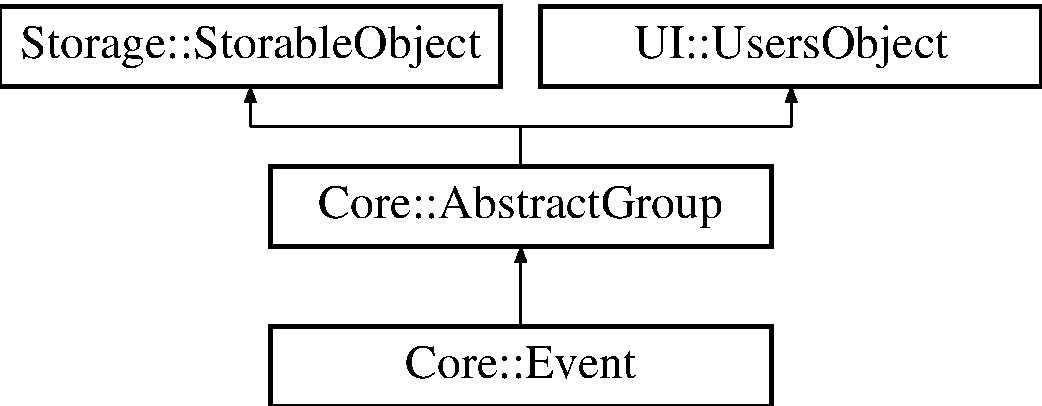
\includegraphics[height=3.000000cm]{d9/d42/classCore_1_1Event}
\end{center}
\end{figure}
\subsection*{Public Member Functions}
\begin{DoxyCompactItemize}
\item 
\hyperlink{classCore_1_1Event_a067e37070ea0fa9b39d7d1171c2f9a2d}{Event} (const int id, \hyperlink{classStorage_1_1AbstractStorage}{Storage::AbstractStorage} \&storage)
\item 
\hyperlink{classCore_1_1Event_aa4a154dde2ab0f1e011fc2f41909cb43}{Event} (const int id, \hyperlink{classStorage_1_1AbstractStorage}{Storage::AbstractStorage} \&storage, const std::string name, const time\_\-t begin, const time\_\-t duration)
\item 
const time\_\-t \hyperlink{classCore_1_1Event_a829b19b781b4d5989928c021b3a3553a}{begin} () const 
\item 
const time\_\-t \hyperlink{classCore_1_1Event_ad83a2109fa632352f63adfdafe2dc86f}{duration} () const 
\item 
const time\_\-t \hyperlink{classCore_1_1Event_af83b91c07834359638a4f7473abad5c5}{end} () const 
\item 
virtual const std::string \hyperlink{classCore_1_1Event_a8dd94bcb05cb3c5ef065fa204cd724f9}{read} () const 
\begin{DoxyCompactList}\small\item\em Returns full object information. \item\end{DoxyCompactList}\item 
virtual const time\_\-t \hyperlink{classCore_1_1Event_a4977832cb03001d8afe46bcddc60ce1a}{read\_\-time} (const std::string name) const   throw (std::bad\_\-cast)
\begin{DoxyCompactList}\small\item\em Return time value of requested field. \item\end{DoxyCompactList}\item 
virtual void \hyperlink{classCore_1_1Event_aaa4b9def6b65cc896e0054210b2d5dae}{update} (const std::string name, const time\_\-t value)  throw (std::bad\_\-cast)
\begin{DoxyCompactList}\small\item\em change current time value of field. \item\end{DoxyCompactList}\item 
virtual void \hyperlink{classCore_1_1Event_a308ae7ad334b8c9a166dc57cfd6a0524}{update} (\hyperlink{classUI_1_1UsersObject}{UI::UsersObject} $\ast$object, const bool linked)  throw (std::bad\_\-cast)
\begin{DoxyCompactList}\small\item\em change current link value of field. \item\end{DoxyCompactList}\end{DoxyCompactItemize}
\subsection*{Protected Member Functions}
\begin{DoxyCompactItemize}
\item 
virtual void \hyperlink{classCore_1_1Event_a6dbea64bf650e7e36d55539cf59a66e7}{save} ()
\begin{DoxyCompactList}\small\item\em Method to save all data in the storage. \item\end{DoxyCompactList}\item 
virtual void \hyperlink{classCore_1_1Event_a63462f7c20234f5c7f18e9c5e19d72b9}{load} ()
\begin{DoxyCompactList}\small\item\em Method to load all data from the storage. \item\end{DoxyCompactList}\end{DoxyCompactItemize}


\subsection{Constructor \& Destructor Documentation}
\hypertarget{classCore_1_1Event_a067e37070ea0fa9b39d7d1171c2f9a2d}{
\index{Core::Event@{Core::Event}!Event@{Event}}
\index{Event@{Event}!Core::Event@{Core::Event}}
\subsubsection[{Event}]{\setlength{\rightskip}{0pt plus 5cm}Core::Event::Event (
\begin{DoxyParamCaption}
\item[{const int}]{id, }
\item[{{\bf Storage::AbstractStorage} \&}]{storage}
\end{DoxyParamCaption}
)\hspace{0.3cm}{\ttfamily  \mbox{[}inline\mbox{]}}}}
\label{d9/d42/classCore_1_1Event_a067e37070ea0fa9b39d7d1171c2f9a2d}
\hypertarget{classCore_1_1Event_aa4a154dde2ab0f1e011fc2f41909cb43}{
\index{Core::Event@{Core::Event}!Event@{Event}}
\index{Event@{Event}!Core::Event@{Core::Event}}
\subsubsection[{Event}]{\setlength{\rightskip}{0pt plus 5cm}Core::Event::Event (
\begin{DoxyParamCaption}
\item[{const int}]{id, }
\item[{{\bf Storage::AbstractStorage} \&}]{storage, }
\item[{const std::string}]{name, }
\item[{const time\_\-t}]{begin, }
\item[{const time\_\-t}]{duration}
\end{DoxyParamCaption}
)\hspace{0.3cm}{\ttfamily  \mbox{[}inline\mbox{]}}}}
\label{d9/d42/classCore_1_1Event_aa4a154dde2ab0f1e011fc2f41909cb43}


\subsection{Member Function Documentation}
\hypertarget{classCore_1_1Event_a829b19b781b4d5989928c021b3a3553a}{
\index{Core::Event@{Core::Event}!begin@{begin}}
\index{begin@{begin}!Core::Event@{Core::Event}}
\subsubsection[{begin}]{\setlength{\rightskip}{0pt plus 5cm}const time\_\-t Core::Event::begin (
\begin{DoxyParamCaption}
{}
\end{DoxyParamCaption}
) const\hspace{0.3cm}{\ttfamily  \mbox{[}inline\mbox{]}}}}
\label{d9/d42/classCore_1_1Event_a829b19b781b4d5989928c021b3a3553a}
\hypertarget{classCore_1_1Event_ad83a2109fa632352f63adfdafe2dc86f}{
\index{Core::Event@{Core::Event}!duration@{duration}}
\index{duration@{duration}!Core::Event@{Core::Event}}
\subsubsection[{duration}]{\setlength{\rightskip}{0pt plus 5cm}const time\_\-t Core::Event::duration (
\begin{DoxyParamCaption}
{}
\end{DoxyParamCaption}
) const\hspace{0.3cm}{\ttfamily  \mbox{[}inline\mbox{]}}}}
\label{d9/d42/classCore_1_1Event_ad83a2109fa632352f63adfdafe2dc86f}
\hypertarget{classCore_1_1Event_af83b91c07834359638a4f7473abad5c5}{
\index{Core::Event@{Core::Event}!end@{end}}
\index{end@{end}!Core::Event@{Core::Event}}
\subsubsection[{end}]{\setlength{\rightskip}{0pt plus 5cm}const time\_\-t Core::Event::end (
\begin{DoxyParamCaption}
{}
\end{DoxyParamCaption}
) const\hspace{0.3cm}{\ttfamily  \mbox{[}inline\mbox{]}}}}
\label{d9/d42/classCore_1_1Event_af83b91c07834359638a4f7473abad5c5}
\hypertarget{classCore_1_1Event_a63462f7c20234f5c7f18e9c5e19d72b9}{
\index{Core::Event@{Core::Event}!load@{load}}
\index{load@{load}!Core::Event@{Core::Event}}
\subsubsection[{load}]{\setlength{\rightskip}{0pt plus 5cm}void Event::load (
\begin{DoxyParamCaption}
{}
\end{DoxyParamCaption}
)\hspace{0.3cm}{\ttfamily  \mbox{[}protected, virtual\mbox{]}}}}
\label{d9/d42/classCore_1_1Event_a63462f7c20234f5c7f18e9c5e19d72b9}


Method to load all data from the storage. 

Declared in the \hyperlink{classStorage_1_1StorableObject}{Storage::StorableObject}. Thil method loads name, child groups and people. Inherited classes must to redefine and coll this one. 

Reimplemented from \hyperlink{classCore_1_1AbstractGroup_ace41b51dd585a95b61990b69f078a283}{Core::AbstractGroup}.

\hypertarget{classCore_1_1Event_a8dd94bcb05cb3c5ef065fa204cd724f9}{
\index{Core::Event@{Core::Event}!read@{read}}
\index{read@{read}!Core::Event@{Core::Event}}
\subsubsection[{read}]{\setlength{\rightskip}{0pt plus 5cm}const std::string Event::read (
\begin{DoxyParamCaption}
{}
\end{DoxyParamCaption}
) const\hspace{0.3cm}{\ttfamily  \mbox{[}virtual\mbox{]}}}}
\label{d9/d42/classCore_1_1Event_a8dd94bcb05cb3c5ef065fa204cd724f9}


Returns full object information. 

\begin{DoxyReturn}{Returns}
Object`s information in the string.
\end{DoxyReturn}
Method declared in the \hyperlink{classUI_1_1UsersObject}{UI::UsersObject} use to retrive all information about object.

Inherited classes must to redefine and call this one. 

Reimplemented from \hyperlink{classCore_1_1AbstractGroup_a0306b58e715d164aef3e29de0ec659bd}{Core::AbstractGroup}.

\hypertarget{classCore_1_1Event_a4977832cb03001d8afe46bcddc60ce1a}{
\index{Core::Event@{Core::Event}!read\_\-time@{read\_\-time}}
\index{read\_\-time@{read\_\-time}!Core::Event@{Core::Event}}
\subsubsection[{read\_\-time}]{\setlength{\rightskip}{0pt plus 5cm}const time\_\-t Event::read\_\-time (
\begin{DoxyParamCaption}
\item[{const std::string}]{name}
\end{DoxyParamCaption}
) const  throw (std::bad\_\-cast)\hspace{0.3cm}{\ttfamily  \mbox{[}virtual\mbox{]}}}}
\label{d9/d42/classCore_1_1Event_a4977832cb03001d8afe46bcddc60ce1a}


Return time value of requested field. 


\begin{DoxyParams}{Parameters}
{\em name} & Name of field which must be returned. Ignored really. \\
\hline
\end{DoxyParams}
\begin{DoxyReturn}{Returns}
Time value of requested field. Never return really.
\end{DoxyReturn}
Call of this method possible from the user interface, but really useless. This method throws std::bad\_\-cast directly. Method used in event class which redefines this. 

Reimplemented from \hyperlink{classCore_1_1AbstractGroup_af52530d29e3b8f0047a0c0675dc6c912}{Core::AbstractGroup}.

\hypertarget{classCore_1_1Event_a6dbea64bf650e7e36d55539cf59a66e7}{
\index{Core::Event@{Core::Event}!save@{save}}
\index{save@{save}!Core::Event@{Core::Event}}
\subsubsection[{save}]{\setlength{\rightskip}{0pt plus 5cm}void Event::save (
\begin{DoxyParamCaption}
{}
\end{DoxyParamCaption}
)\hspace{0.3cm}{\ttfamily  \mbox{[}protected, virtual\mbox{]}}}}
\label{d9/d42/classCore_1_1Event_a6dbea64bf650e7e36d55539cf59a66e7}


Method to save all data in the storage. 

Declared in the \hyperlink{classStorage_1_1StorableObject}{Storage::StorableObject}. This method saves name, child groups and people. Inherited classes must to redefine and call this one. 

Reimplemented from \hyperlink{classCore_1_1AbstractGroup_ab8cc5ad1c04d67c24af785f9adb2d67c}{Core::AbstractGroup}.

\hypertarget{classCore_1_1Event_a308ae7ad334b8c9a166dc57cfd6a0524}{
\index{Core::Event@{Core::Event}!update@{update}}
\index{update@{update}!Core::Event@{Core::Event}}
\subsubsection[{update}]{\setlength{\rightskip}{0pt plus 5cm}void Event::update (
\begin{DoxyParamCaption}
\item[{{\bf UI::UsersObject} $\ast$}]{object, }
\item[{const bool}]{linked}
\end{DoxyParamCaption}
)  throw (std::bad\_\-cast)\hspace{0.3cm}{\ttfamily  \mbox{[}virtual\mbox{]}}}}
\label{d9/d42/classCore_1_1Event_a308ae7ad334b8c9a166dc57cfd6a0524}


change current link value of field. 


\begin{DoxyParams}{Parameters}
{\em object} & Object link with that must be changed. \\
\hline
{\em linked} & New state of thi link.\\
\hline
\end{DoxyParams}
This method tries to add or delete object to the group as the \hyperlink{classCore_1_1Person}{Person}. dynamic\_\-cast will throw std::bad\_\-cast if object is not \hyperlink{classCore_1_1Person}{Person}.

You can not set child group by this method use redefined method in \hyperlink{classCore_1_1Group}{Group} class to add parent group. 

Reimplemented from \hyperlink{classCore_1_1AbstractGroup_a1b3a59bf11da1ea7bd9a0735cb54dbb8}{Core::AbstractGroup}.

\hypertarget{classCore_1_1Event_aaa4b9def6b65cc896e0054210b2d5dae}{
\index{Core::Event@{Core::Event}!update@{update}}
\index{update@{update}!Core::Event@{Core::Event}}
\subsubsection[{update}]{\setlength{\rightskip}{0pt plus 5cm}void Event::update (
\begin{DoxyParamCaption}
\item[{const std::string}]{name, }
\item[{const time\_\-t}]{value}
\end{DoxyParamCaption}
)  throw (std::bad\_\-cast)\hspace{0.3cm}{\ttfamily  \mbox{[}virtual\mbox{]}}}}
\label{d9/d42/classCore_1_1Event_aaa4b9def6b65cc896e0054210b2d5dae}


change current time value of field. 


\begin{DoxyParams}{Parameters}
{\em name} & Name of field which must be changed. Ignored really. \\
\hline
{\em value} & New value of field. Ignored really.\\
\hline
\end{DoxyParams}
Call of this method possible from the user interface, but really useless. This method throws std::bad\_\-cast directly. \hyperlink{classCore_1_1Event}{Event} class must to redefine this one. 

Reimplemented from \hyperlink{classCore_1_1AbstractGroup_a9891a3850584dc3677563aea603fb9c2}{Core::AbstractGroup}.



The documentation for this class was generated from the following files:\begin{DoxyCompactItemize}
\item 
src/include/\hyperlink{include_2event_8h}{event.h}\item 
src/core/\hyperlink{core_2event_8cpp}{event.cpp}\end{DoxyCompactItemize}

\hypertarget{classCore_1_1Group}{
\section{Core::Group Class Reference}
\label{d2/d30/classCore_1_1Group}\index{Core::Group@{Core::Group}}
}


Class keeps information about group of people.  




{\ttfamily \#include $<$group.h$>$}



Inheritance diagram for Core::Group:
\nopagebreak
\begin{figure}[H]
\begin{center}
\leavevmode
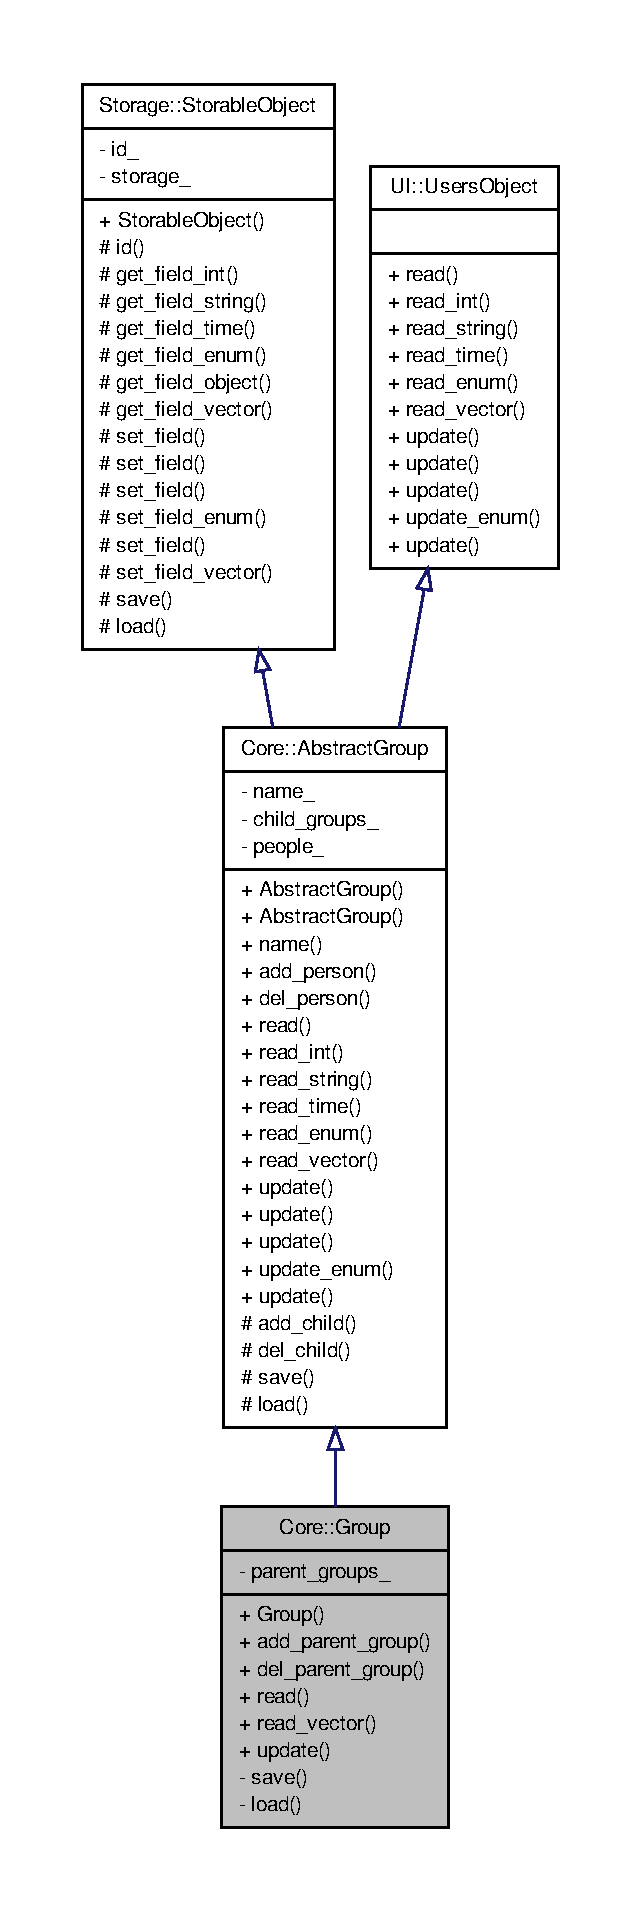
\includegraphics[height=600pt]{d6/d15/classCore_1_1Group__inherit__graph}
\end{center}
\end{figure}


Collaboration diagram for Core::Group:
\nopagebreak
\begin{figure}[H]
\begin{center}
\leavevmode
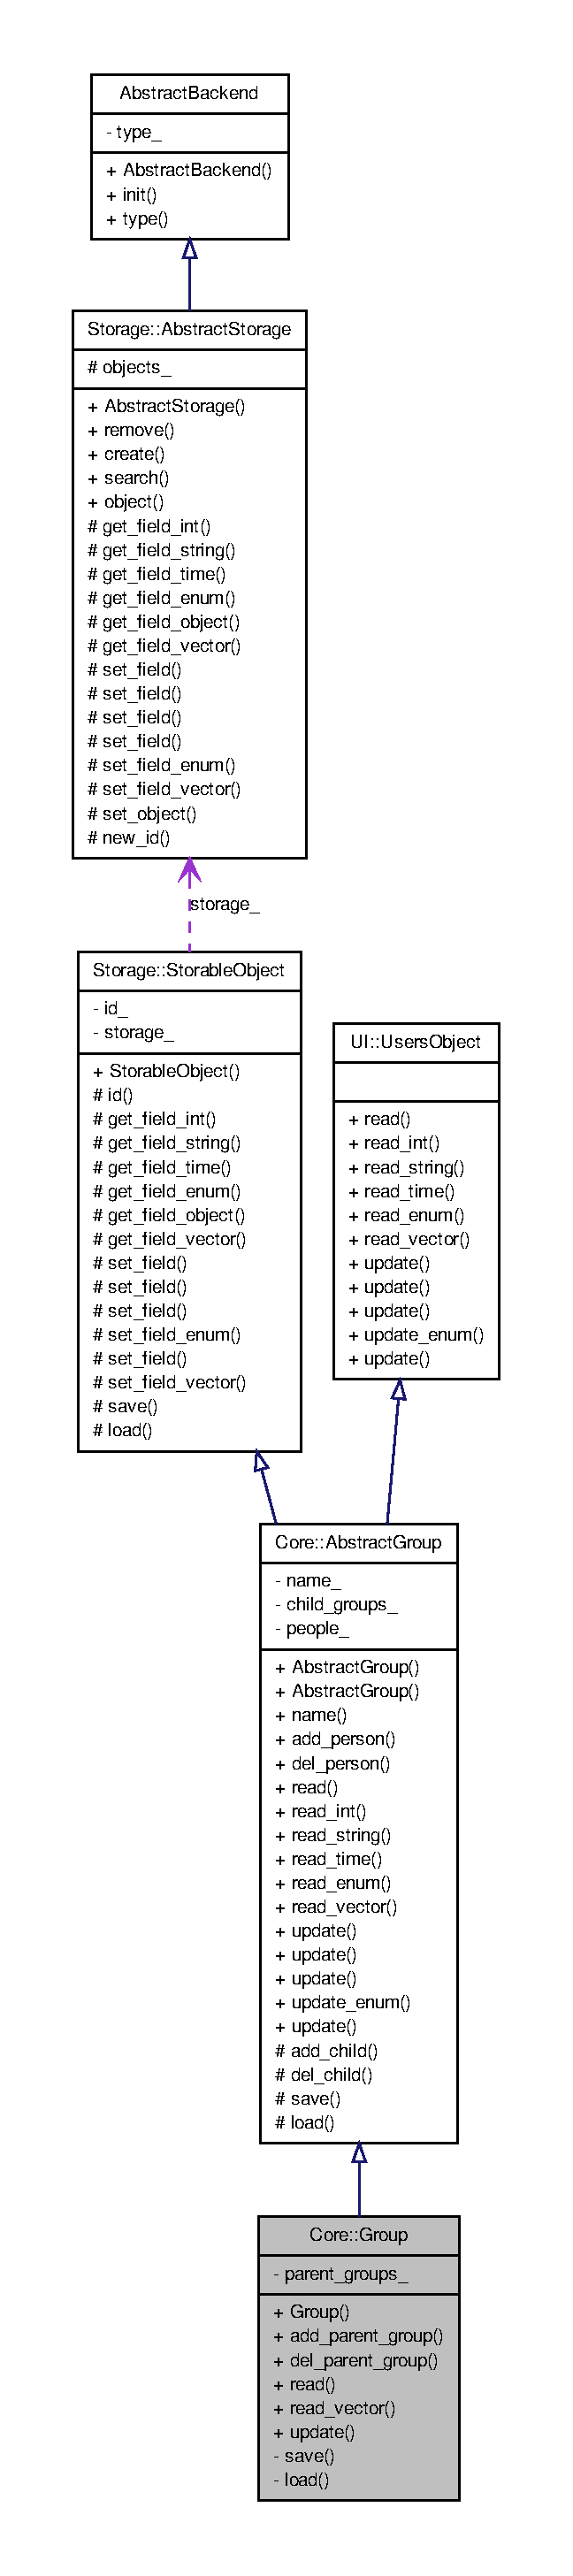
\includegraphics[height=600pt]{d7/da7/classCore_1_1Group__coll__graph}
\end{center}
\end{figure}
\subsection*{Public Member Functions}
\begin{DoxyCompactItemize}
\item 
\hyperlink{classCore_1_1Group_a39511a091570283cb5fb2a4b8f0a841a}{Group} (const int id, \hyperlink{classStorage_1_1AbstractStorage}{Storage::AbstractStorage} \&storage)
\item 
void \hyperlink{classCore_1_1Group_a05760e4e45ae6fec2674d216f0a5a6e9}{add\_\-parent\_\-group} (\hyperlink{classCore_1_1AbstractGroup}{AbstractGroup} $\ast$group)
\item 
void \hyperlink{classCore_1_1Group_a93e4626dde0f84e68f1460e557daaed0}{del\_\-parent\_\-group} (\hyperlink{classCore_1_1AbstractGroup}{AbstractGroup} $\ast$group)
\item 
virtual const std::string \hyperlink{classCore_1_1Group_a5fe3fef1b6709f953e5487841d90bbb9}{read} () const 
\begin{DoxyCompactList}\small\item\em Returns full object information. \item\end{DoxyCompactList}\item 
virtual const std::vector$<$ \hyperlink{classUI_1_1UsersObject}{UI::UsersObject} $\ast$ $>$ \hyperlink{classCore_1_1Group_a52e48b1f92f6354b4e3a32d710b9c7b3}{read\_\-vector} (const std::string name) const   throw (std::bad\_\-cast)
\begin{DoxyCompactList}\small\item\em Return vector value of requested field. \item\end{DoxyCompactList}\item 
virtual void \hyperlink{classCore_1_1Group_a12d2636d65f1baea3666bb492320b5c1}{update} (\hyperlink{classUI_1_1UsersObject}{UI::UsersObject} $\ast$object, const bool linked)  throw (std::bad\_\-cast)
\begin{DoxyCompactList}\small\item\em change current link value of field. \item\end{DoxyCompactList}\end{DoxyCompactItemize}


\subsection{Detailed Description}
Class keeps information about group of people. $<$ 

\subsection{Constructor \& Destructor Documentation}
\hypertarget{classCore_1_1Group_a39511a091570283cb5fb2a4b8f0a841a}{
\index{Core::Group@{Core::Group}!Group@{Group}}
\index{Group@{Group}!Core::Group@{Core::Group}}
\subsubsection[{Group}]{\setlength{\rightskip}{0pt plus 5cm}Core::Group::Group (
\begin{DoxyParamCaption}
\item[{const int}]{id, }
\item[{{\bf Storage::AbstractStorage} \&}]{storage}
\end{DoxyParamCaption}
)\hspace{0.3cm}{\ttfamily  \mbox{[}inline\mbox{]}}}}
\label{d2/d30/classCore_1_1Group_a39511a091570283cb5fb2a4b8f0a841a}


\subsection{Member Function Documentation}
\hypertarget{classCore_1_1Group_a05760e4e45ae6fec2674d216f0a5a6e9}{
\index{Core::Group@{Core::Group}!add\_\-parent\_\-group@{add\_\-parent\_\-group}}
\index{add\_\-parent\_\-group@{add\_\-parent\_\-group}!Core::Group@{Core::Group}}
\subsubsection[{add\_\-parent\_\-group}]{\setlength{\rightskip}{0pt plus 5cm}void Group::add\_\-parent\_\-group (
\begin{DoxyParamCaption}
\item[{{\bf AbstractGroup} $\ast$}]{group}
\end{DoxyParamCaption}
)}}
\label{d2/d30/classCore_1_1Group_a05760e4e45ae6fec2674d216f0a5a6e9}


Here is the call graph for this function:
\nopagebreak
\begin{figure}[H]
\begin{center}
\leavevmode
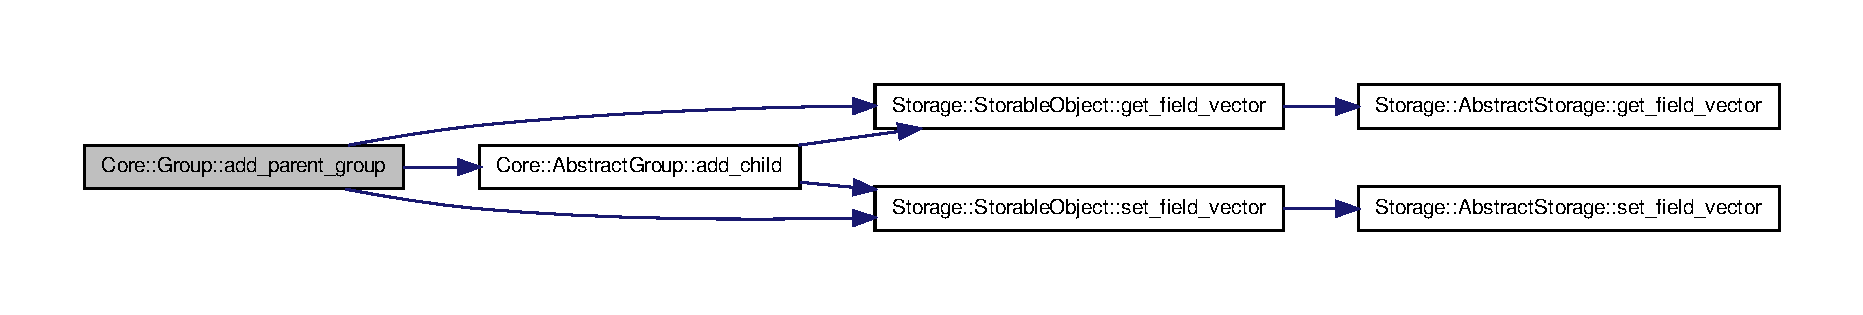
\includegraphics[width=400pt]{d2/d30/classCore_1_1Group_a05760e4e45ae6fec2674d216f0a5a6e9_cgraph}
\end{center}
\end{figure}


\hypertarget{classCore_1_1Group_a93e4626dde0f84e68f1460e557daaed0}{
\index{Core::Group@{Core::Group}!del\_\-parent\_\-group@{del\_\-parent\_\-group}}
\index{del\_\-parent\_\-group@{del\_\-parent\_\-group}!Core::Group@{Core::Group}}
\subsubsection[{del\_\-parent\_\-group}]{\setlength{\rightskip}{0pt plus 5cm}void Group::del\_\-parent\_\-group (
\begin{DoxyParamCaption}
\item[{{\bf AbstractGroup} $\ast$}]{group}
\end{DoxyParamCaption}
)}}
\label{d2/d30/classCore_1_1Group_a93e4626dde0f84e68f1460e557daaed0}


Here is the call graph for this function:
\nopagebreak
\begin{figure}[H]
\begin{center}
\leavevmode
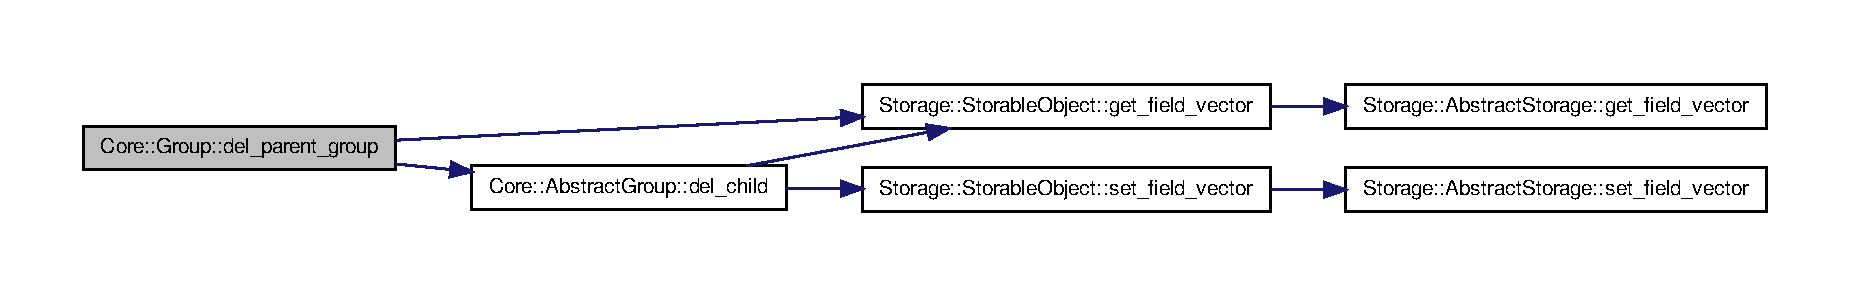
\includegraphics[width=400pt]{d2/d30/classCore_1_1Group_a93e4626dde0f84e68f1460e557daaed0_cgraph}
\end{center}
\end{figure}


\hypertarget{classCore_1_1Group_a5fe3fef1b6709f953e5487841d90bbb9}{
\index{Core::Group@{Core::Group}!read@{read}}
\index{read@{read}!Core::Group@{Core::Group}}
\subsubsection[{read}]{\setlength{\rightskip}{0pt plus 5cm}const std::string Group::read (
\begin{DoxyParamCaption}
{}
\end{DoxyParamCaption}
) const\hspace{0.3cm}{\ttfamily  \mbox{[}virtual\mbox{]}}}}
\label{d2/d30/classCore_1_1Group_a5fe3fef1b6709f953e5487841d90bbb9}


Returns full object information. 

\begin{DoxyReturn}{Returns}
Object`s information in the string.
\end{DoxyReturn}
Method declared in the \hyperlink{classUI_1_1UsersObject}{UI::UsersObject} use to retrive all information about object.

Inherited classes must to redefine and call this one. 

Reimplemented from \hyperlink{classCore_1_1AbstractGroup_a0306b58e715d164aef3e29de0ec659bd}{Core::AbstractGroup}.

\hypertarget{classCore_1_1Group_a52e48b1f92f6354b4e3a32d710b9c7b3}{
\index{Core::Group@{Core::Group}!read\_\-vector@{read\_\-vector}}
\index{read\_\-vector@{read\_\-vector}!Core::Group@{Core::Group}}
\subsubsection[{read\_\-vector}]{\setlength{\rightskip}{0pt plus 5cm}const std::vector$<$ {\bf UI::UsersObject} $\ast$ $>$ Group::read\_\-vector (
\begin{DoxyParamCaption}
\item[{const std::string}]{name}
\end{DoxyParamCaption}
) const  throw (std::bad\_\-cast)\hspace{0.3cm}{\ttfamily  \mbox{[}virtual\mbox{]}}}}
\label{d2/d30/classCore_1_1Group_a52e48b1f92f6354b4e3a32d710b9c7b3}


Return vector value of requested field. 


\begin{DoxyParams}{Parameters}
{\em name} & Name of field which must be returned. \\
\hline
\end{DoxyParams}
\begin{DoxyReturn}{Returns}
Vector value of requested field.
\end{DoxyReturn}
Use this for child\_\-groups and people fields. Throws exception in the other cases. 

Reimplemented from \hyperlink{classCore_1_1AbstractGroup_ab582f4364426a152875742278ba0d999}{Core::AbstractGroup}.



Here is the call graph for this function:
\nopagebreak
\begin{figure}[H]
\begin{center}
\leavevmode
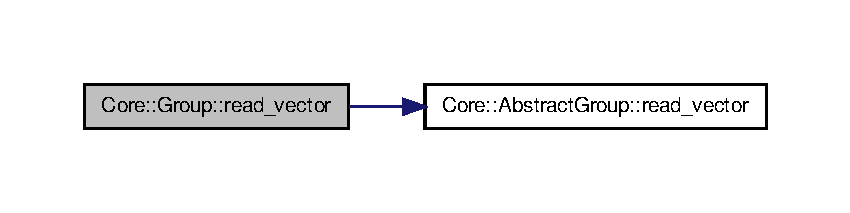
\includegraphics[width=400pt]{d2/d30/classCore_1_1Group_a52e48b1f92f6354b4e3a32d710b9c7b3_cgraph}
\end{center}
\end{figure}


\hypertarget{classCore_1_1Group_a12d2636d65f1baea3666bb492320b5c1}{
\index{Core::Group@{Core::Group}!update@{update}}
\index{update@{update}!Core::Group@{Core::Group}}
\subsubsection[{update}]{\setlength{\rightskip}{0pt plus 5cm}void Group::update (
\begin{DoxyParamCaption}
\item[{{\bf UI::UsersObject} $\ast$}]{object, }
\item[{const bool}]{linked}
\end{DoxyParamCaption}
)  throw (std::bad\_\-cast)\hspace{0.3cm}{\ttfamily  \mbox{[}virtual\mbox{]}}}}
\label{d2/d30/classCore_1_1Group_a12d2636d65f1baea3666bb492320b5c1}


change current link value of field. 


\begin{DoxyParams}{Parameters}
{\em object} & Object link with that must be changed. \\
\hline
{\em linked} & New state of thi link.\\
\hline
\end{DoxyParams}
This method tries to add or delete object to the group as the \hyperlink{classCore_1_1Person}{Person}. dynamic\_\-cast will throw std::bad\_\-cast if object is not \hyperlink{classCore_1_1Person}{Person}.

You can not set child group by this method use redefined method in \hyperlink{classCore_1_1Group}{Group} class to add parent group. 

Reimplemented from \hyperlink{classCore_1_1AbstractGroup_a1b3a59bf11da1ea7bd9a0735cb54dbb8}{Core::AbstractGroup}.



Here is the call graph for this function:
\nopagebreak
\begin{figure}[H]
\begin{center}
\leavevmode
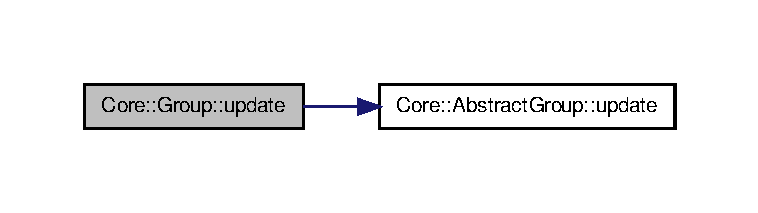
\includegraphics[width=364pt]{d2/d30/classCore_1_1Group_a12d2636d65f1baea3666bb492320b5c1_cgraph}
\end{center}
\end{figure}




The documentation for this class was generated from the following files:\begin{DoxyCompactItemize}
\item 
src/include/\hyperlink{group_8h}{group.h}\item 
src/core/\hyperlink{group_8cpp}{group.cpp}\end{DoxyCompactItemize}

\hypertarget{classCore_1_1Person}{
\section{Core::Person Class Reference}
\label{d9/d71/classCore_1_1Person}\index{Core::Person@{Core::Person}}
}


Class keeps person unique data.  




{\ttfamily \#include $<$person.h$>$}



Inheritance diagram for Core::Person:
\nopagebreak
\begin{figure}[H]
\begin{center}
\leavevmode
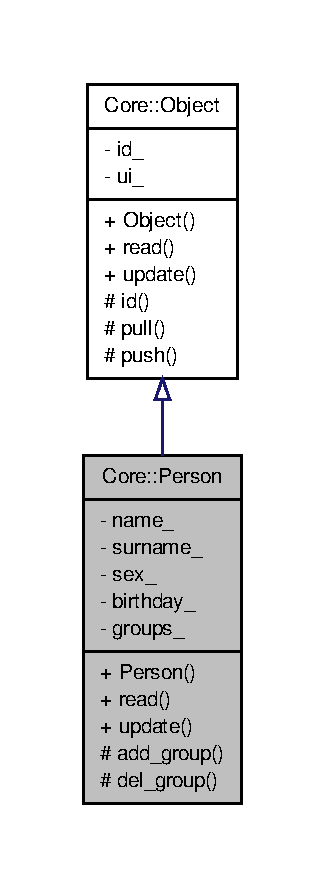
\includegraphics[height=600pt]{d0/dc4/classCore_1_1Person__inherit__graph}
\end{center}
\end{figure}


Collaboration diagram for Core::Person:
\nopagebreak
\begin{figure}[H]
\begin{center}
\leavevmode
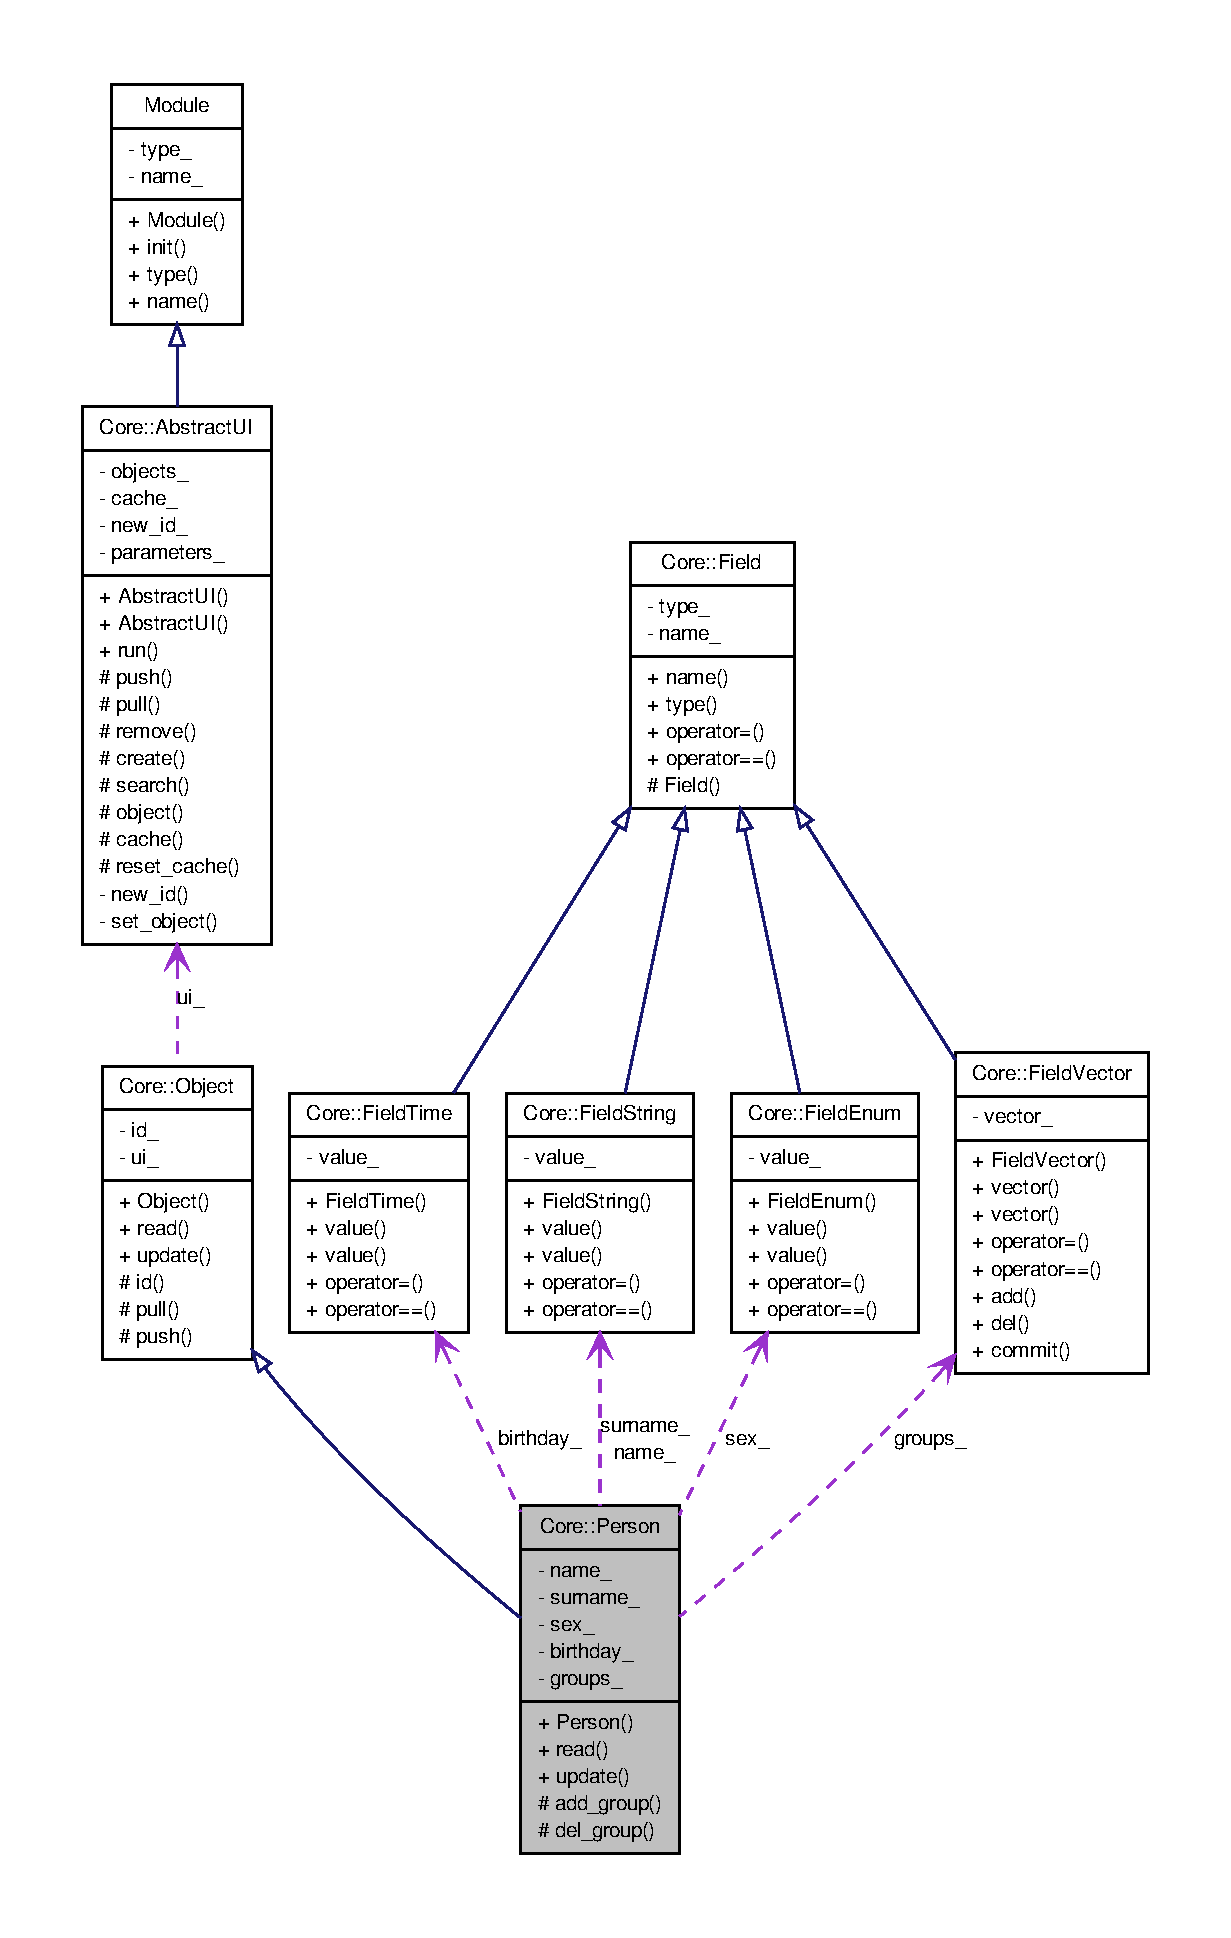
\includegraphics[height=600pt]{dc/d29/classCore_1_1Person__coll__graph}
\end{center}
\end{figure}
\subsection*{Public Types}
\begin{DoxyCompactItemize}
\item 
enum \hyperlink{classCore_1_1Person_a01e6eee93727f9ce06525eca689b4764}{Sex} \{ \hyperlink{classCore_1_1Person_a01e6eee93727f9ce06525eca689b4764aeb7355bb082d0aa0d2b315e5dfaa2de9}{MALE}, 
\hyperlink{classCore_1_1Person_a01e6eee93727f9ce06525eca689b4764a0c4f3aef529b75d197d411a6336ec3a1}{FEMALE}
 \}
\end{DoxyCompactItemize}
\subsection*{Public Member Functions}
\begin{DoxyCompactItemize}
\item 
\hyperlink{classCore_1_1Person_a3f7bca52408bae72dd0213b2a92827f0}{Person} (const int id, \hyperlink{classStorage_1_1AbstractStorage}{Storage::AbstractStorage} \&storage)
\item 
\hyperlink{classCore_1_1Person_aa1b55740d1dd9f2543ad27f4ecca8e72}{Person} (const int id, \hyperlink{classStorage_1_1AbstractStorage}{Storage::AbstractStorage} \&storage, const std::string name, const std::string surname, const enum \hyperlink{classCore_1_1Person_a01e6eee93727f9ce06525eca689b4764}{Sex} sex, const time\_\-t birthday)
\item 
const std::string \hyperlink{classCore_1_1Person_a14d39111fb34383818154a26b0d248f5}{name} () const 
\item 
const std::string \hyperlink{classCore_1_1Person_a5572207d53649af10cd9bb62fe21995c}{surname} () const 
\item 
enum \hyperlink{classCore_1_1Person_a01e6eee93727f9ce06525eca689b4764}{Sex} \hyperlink{classCore_1_1Person_a0d70ad24edf86e3c0f88e913342aa24d}{sex} () const 
\item 
const time\_\-t \hyperlink{classCore_1_1Person_ab0d1836a97254798585fc6c97a63680e}{birthday} () const 
\item 
const std::vector$<$ class \hyperlink{classCore_1_1AbstractGroup}{AbstractGroup} $\ast$ $>$ \& \hyperlink{classCore_1_1Person_ae6dc9f0c0ca2caf326b69b72d81aea84}{groups} ()
\item 
virtual const std::string \hyperlink{classCore_1_1Person_a3b86cab797444527364376dad2a0c300}{read} () const 
\item 
virtual const int \hyperlink{classCore_1_1Person_a9b1601502537f54b7c33fc593f8df590}{read\_\-int} (const std::string name) const   throw (std::bad\_\-cast)
\item 
virtual const std::string \hyperlink{classCore_1_1Person_a4b7d0b1c545c2c4876b3f410b914f3a2}{read\_\-string} (const std::string name) const   throw (std::bad\_\-cast)
\item 
virtual const time\_\-t \hyperlink{classCore_1_1Person_ad0485ff28f4f80aeb0da9f8a6ae2f6d0}{read\_\-time} (const std::string name) const   throw (std::bad\_\-cast)
\item 
virtual const std::string \hyperlink{classCore_1_1Person_a5dfa21d7b0a58e09f71e07a4298f0f62}{read\_\-enum} (const std::string name) const   throw (std::bad\_\-cast)
\item 
virtual const std::vector$<$ \hyperlink{classUI_1_1UsersObject}{UI::UsersObject} $\ast$ $>$ \hyperlink{classCore_1_1Person_ab28c3e468d265c16bce1d4488493c5a6}{read\_\-vector} (const std::string name) const   throw (std::bad\_\-cast)
\item 
virtual void \hyperlink{classCore_1_1Person_ac2900dc24258c00ea1de17350c3f4658}{update} (const std::string name, const int value)  throw (std::bad\_\-cast)
\item 
virtual void \hyperlink{classCore_1_1Person_a51ec02307587cf9dfd7ed3036cf202cd}{update} (const std::string name, const std::string value)  throw (std::bad\_\-cast)
\item 
virtual void \hyperlink{classCore_1_1Person_ad650eba89f671041c26f8d1419f6e6c8}{update} (const std::string name, const time\_\-t value)  throw (std::bad\_\-cast)
\item 
virtual void \hyperlink{classCore_1_1Person_a1c6826659c2413189dae536f7c83af98}{update\_\-enum} (const std::string, const std::string value)  throw (std::bad\_\-cast)
\item 
virtual void \hyperlink{classCore_1_1Person_a50fa1e127f56e2caa873017b54c090cb}{update} (UsersObject $\ast$, bool linked)  throw (std::bad\_\-cast)
\end{DoxyCompactItemize}
\subsection*{Static Public Member Functions}
\begin{DoxyCompactItemize}
\item 
static const \hyperlink{classCore_1_1Person_a01e6eee93727f9ce06525eca689b4764}{Sex} \hyperlink{classCore_1_1Person_a88e1d40e7be7d95e6cec9bc623d6e076}{\_\-} (const std::string str)
\item 
static const std::string \hyperlink{classCore_1_1Person_a7ded3b871b2e7f6ce35b7b1f4e1738ee}{\_\-} (const \hyperlink{classCore_1_1Person_a01e6eee93727f9ce06525eca689b4764}{Sex} sex)
\end{DoxyCompactItemize}
\subsection*{Protected Member Functions}
\begin{DoxyCompactItemize}
\item 
void \hyperlink{classCore_1_1Person_aa9b9581966365e7272d43e77f7a220e4}{add\_\-group} (class \hyperlink{classCore_1_1AbstractGroup}{AbstractGroup} $\ast$group)
\item 
void \hyperlink{classCore_1_1Person_a0057f7bd335dd35e470e67ad2e22b0d5}{del\_\-group} (class \hyperlink{classCore_1_1AbstractGroup}{AbstractGroup} const $\ast$group)
\item 
void \hyperlink{classCore_1_1Person_a846fa55a79f6da0258d711adc88a1a30}{save} ()
\item 
void \hyperlink{classCore_1_1Person_ae88c1b9c89b03ac7f4ba3ddcff4c62a7}{load} ()
\end{DoxyCompactItemize}
\subsection*{Friends}
\begin{DoxyCompactItemize}
\item 
class \hyperlink{classCore_1_1Person_a8be971ab18693e55f617c7dc8abc3e26}{AbstractGroup}
\end{DoxyCompactItemize}


\subsection{Detailed Description}
Class keeps person unique data. 

\subsection{Member Enumeration Documentation}
\hypertarget{classCore_1_1Person_a01e6eee93727f9ce06525eca689b4764}{
\index{Core::Person@{Core::Person}!Sex@{Sex}}
\index{Sex@{Sex}!Core::Person@{Core::Person}}
\subsubsection[{Sex}]{\setlength{\rightskip}{0pt plus 5cm}enum {\bf Core::Person::Sex}}}
\label{d9/d71/classCore_1_1Person_a01e6eee93727f9ce06525eca689b4764}
enum of sex \begin{Desc}
\item[Enumerator: ]\par
\begin{description}
\index{MALE@{MALE}!Core::Person@{Core::Person}}\index{Core::Person@{Core::Person}!MALE@{MALE}}\item[{\em 
\hypertarget{classCore_1_1Person_a01e6eee93727f9ce06525eca689b4764aeb7355bb082d0aa0d2b315e5dfaa2de9}{
MALE}
\label{d9/d71/classCore_1_1Person_a01e6eee93727f9ce06525eca689b4764aeb7355bb082d0aa0d2b315e5dfaa2de9}
}]\index{FEMALE@{FEMALE}!Core::Person@{Core::Person}}\index{Core::Person@{Core::Person}!FEMALE@{FEMALE}}\item[{\em 
\hypertarget{classCore_1_1Person_a01e6eee93727f9ce06525eca689b4764a0c4f3aef529b75d197d411a6336ec3a1}{
FEMALE}
\label{d9/d71/classCore_1_1Person_a01e6eee93727f9ce06525eca689b4764a0c4f3aef529b75d197d411a6336ec3a1}
}]\end{description}
\end{Desc}



\subsection{Constructor \& Destructor Documentation}
\hypertarget{classCore_1_1Person_a3f7bca52408bae72dd0213b2a92827f0}{
\index{Core::Person@{Core::Person}!Person@{Person}}
\index{Person@{Person}!Core::Person@{Core::Person}}
\subsubsection[{Person}]{\setlength{\rightskip}{0pt plus 5cm}Core::Person::Person (
\begin{DoxyParamCaption}
\item[{const int}]{id, }
\item[{{\bf Storage::AbstractStorage} \&}]{storage}
\end{DoxyParamCaption}
)\hspace{0.3cm}{\ttfamily  \mbox{[}inline\mbox{]}}}}
\label{d9/d71/classCore_1_1Person_a3f7bca52408bae72dd0213b2a92827f0}
Constructor. Call at \hyperlink{classStorage_1_1AbstractStorage_a108af124f19c0ae9a4a461aee6abc3ec}{Storage::AbstractStorage::create$<$Person$>$()}. 
\begin{DoxyParams}[1]{Parameters}
\mbox{\tt in}  & {\em id} & Person's identificator. \\
\hline
\mbox{\tt in}  & {\em storage} & Data storage. \\
\hline
\end{DoxyParams}
\hypertarget{classCore_1_1Person_aa1b55740d1dd9f2543ad27f4ecca8e72}{
\index{Core::Person@{Core::Person}!Person@{Person}}
\index{Person@{Person}!Core::Person@{Core::Person}}
\subsubsection[{Person}]{\setlength{\rightskip}{0pt plus 5cm}Core::Person::Person (
\begin{DoxyParamCaption}
\item[{const int}]{id, }
\item[{{\bf Storage::AbstractStorage} \&}]{storage, }
\item[{const std::string}]{name, }
\item[{const std::string}]{surname, }
\item[{const enum {\bf Sex}}]{sex, }
\item[{const time\_\-t}]{birthday}
\end{DoxyParamCaption}
)\hspace{0.3cm}{\ttfamily  \mbox{[}inline\mbox{]}}}}
\label{d9/d71/classCore_1_1Person_aa1b55740d1dd9f2543ad27f4ecca8e72}
\begin{Desc}
\item[\hyperlink{deprecated__deprecated000003}{Deprecated}]Constructor. \end{Desc}

\begin{DoxyParams}[1]{Parameters}
\mbox{\tt in}  & {\em id} & Person's identificator. \\
\hline
\mbox{\tt in}  & {\em storage} & Data storage. \\
\hline
\mbox{\tt in}  & {\em name} & Person's name. \\
\hline
\mbox{\tt in}  & {\em surname} & Person's surname. \\
\hline
\mbox{\tt in}  & {\em sex} & Person's sex. \\
\hline
\mbox{\tt in}  & {\em birthday} & Person's birthday. \\
\hline
\end{DoxyParams}


\subsection{Member Function Documentation}
\hypertarget{classCore_1_1Person_a88e1d40e7be7d95e6cec9bc623d6e076}{
\index{Core::Person@{Core::Person}!\_\-@{\_\-}}
\index{\_\-@{\_\-}!Core::Person@{Core::Person}}
\subsubsection[{\_\-}]{\setlength{\rightskip}{0pt plus 5cm}static const {\bf Sex} Core::Person::\_\- (
\begin{DoxyParamCaption}
\item[{const std::string}]{str}
\end{DoxyParamCaption}
)\hspace{0.3cm}{\ttfamily  \mbox{[}inline, static\mbox{]}}}}
\label{d9/d71/classCore_1_1Person_a88e1d40e7be7d95e6cec9bc623d6e076}
Small function to easy type casting. 
\begin{DoxyParams}[1]{Parameters}
\mbox{\tt in}  & {\em str} & String to cast. \\
\hline
\end{DoxyParams}
\begin{DoxyReturn}{Returns}
MALE if string equals to \char`\"{}MALE\char`\"{} else FEMALE. 
\end{DoxyReturn}


Here is the caller graph for this function:
\nopagebreak
\begin{figure}[H]
\begin{center}
\leavevmode
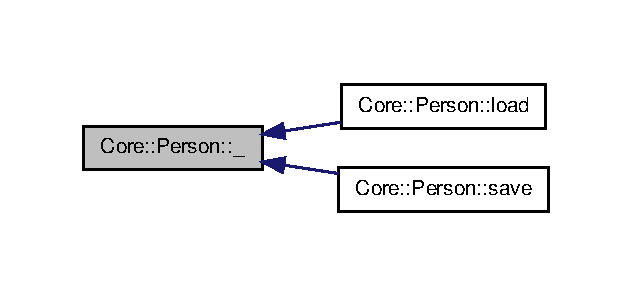
\includegraphics[width=304pt]{d9/d71/classCore_1_1Person_a88e1d40e7be7d95e6cec9bc623d6e076_icgraph}
\end{center}
\end{figure}


\hypertarget{classCore_1_1Person_a7ded3b871b2e7f6ce35b7b1f4e1738ee}{
\index{Core::Person@{Core::Person}!\_\-@{\_\-}}
\index{\_\-@{\_\-}!Core::Person@{Core::Person}}
\subsubsection[{\_\-}]{\setlength{\rightskip}{0pt plus 5cm}static const std::string Core::Person::\_\- (
\begin{DoxyParamCaption}
\item[{const {\bf Sex}}]{sex}
\end{DoxyParamCaption}
)\hspace{0.3cm}{\ttfamily  \mbox{[}inline, static\mbox{]}}}}
\label{d9/d71/classCore_1_1Person_a7ded3b871b2e7f6ce35b7b1f4e1738ee}
Small function to easy type casting. 
\begin{DoxyParams}[1]{Parameters}
\mbox{\tt in}  & {\em sex} & enum to cast. \\
\hline
\end{DoxyParams}
\begin{DoxyReturn}{Returns}
\char`\"{}MALE\char`\"{} if enum equals to MALE else FEMALE. 
\end{DoxyReturn}
\hypertarget{classCore_1_1Person_aa9b9581966365e7272d43e77f7a220e4}{
\index{Core::Person@{Core::Person}!add\_\-group@{add\_\-group}}
\index{add\_\-group@{add\_\-group}!Core::Person@{Core::Person}}
\subsubsection[{add\_\-group}]{\setlength{\rightskip}{0pt plus 5cm}void Core::Person::add\_\-group (
\begin{DoxyParamCaption}
\item[{class {\bf AbstractGroup} $\ast$}]{group}
\end{DoxyParamCaption}
)\hspace{0.3cm}{\ttfamily  \mbox{[}inline, protected\mbox{]}}}}
\label{d9/d71/classCore_1_1Person_aa9b9581966365e7272d43e77f7a220e4}
Add group to person, call in \hyperlink{classCore_1_1AbstractGroup_a8c59706bf4c5f8e6dc8f931368d97b7f}{AbstractGroup::add\_\-person()} 
\begin{DoxyParams}[1]{Parameters}
\mbox{\tt in}  & {\em group} & to add. \\
\hline
\end{DoxyParams}


Here is the caller graph for this function:
\nopagebreak
\begin{figure}[H]
\begin{center}
\leavevmode
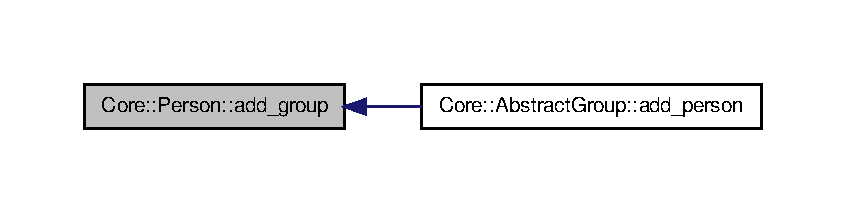
\includegraphics[width=400pt]{d9/d71/classCore_1_1Person_aa9b9581966365e7272d43e77f7a220e4_icgraph}
\end{center}
\end{figure}


\hypertarget{classCore_1_1Person_ab0d1836a97254798585fc6c97a63680e}{
\index{Core::Person@{Core::Person}!birthday@{birthday}}
\index{birthday@{birthday}!Core::Person@{Core::Person}}
\subsubsection[{birthday}]{\setlength{\rightskip}{0pt plus 5cm}const time\_\-t Core::Person::birthday (
\begin{DoxyParamCaption}
{}
\end{DoxyParamCaption}
) const\hspace{0.3cm}{\ttfamily  \mbox{[}inline\mbox{]}}}}
\label{d9/d71/classCore_1_1Person_ab0d1836a97254798585fc6c97a63680e}
\begin{Desc}
\item[\hyperlink{deprecated__deprecated000007}{Deprecated}]Get birthday of person. \end{Desc}
\begin{DoxyReturn}{Returns}
person's birthday. 
\end{DoxyReturn}
\hypertarget{classCore_1_1Person_a0057f7bd335dd35e470e67ad2e22b0d5}{
\index{Core::Person@{Core::Person}!del\_\-group@{del\_\-group}}
\index{del\_\-group@{del\_\-group}!Core::Person@{Core::Person}}
\subsubsection[{del\_\-group}]{\setlength{\rightskip}{0pt plus 5cm}void Person::del\_\-group (
\begin{DoxyParamCaption}
\item[{class {\bf AbstractGroup} const $\ast$}]{group}
\end{DoxyParamCaption}
)\hspace{0.3cm}{\ttfamily  \mbox{[}protected\mbox{]}}}}
\label{d9/d71/classCore_1_1Person_a0057f7bd335dd35e470e67ad2e22b0d5}
Delete group from person. 
\begin{DoxyParams}[1]{Parameters}
\mbox{\tt in}  & {\em group.} & \\
\hline
\end{DoxyParams}
\hypertarget{classCore_1_1Person_ae6dc9f0c0ca2caf326b69b72d81aea84}{
\index{Core::Person@{Core::Person}!groups@{groups}}
\index{groups@{groups}!Core::Person@{Core::Person}}
\subsubsection[{groups}]{\setlength{\rightskip}{0pt plus 5cm}const std::vector$<$class {\bf AbstractGroup} $\ast$$>$\& Core::Person::groups (
\begin{DoxyParamCaption}
{}
\end{DoxyParamCaption}
)\hspace{0.3cm}{\ttfamily  \mbox{[}inline\mbox{]}}}}
\label{d9/d71/classCore_1_1Person_ae6dc9f0c0ca2caf326b69b72d81aea84}
\begin{Desc}
\item[\hyperlink{deprecated__deprecated000008}{Deprecated}]Get person's groups. \end{Desc}
\begin{DoxyReturn}{Returns}
person's groups. 
\end{DoxyReturn}
\hypertarget{classCore_1_1Person_ae88c1b9c89b03ac7f4ba3ddcff4c62a7}{
\index{Core::Person@{Core::Person}!load@{load}}
\index{load@{load}!Core::Person@{Core::Person}}
\subsubsection[{load}]{\setlength{\rightskip}{0pt plus 5cm}void Person::load (
\begin{DoxyParamCaption}
{}
\end{DoxyParamCaption}
)\hspace{0.3cm}{\ttfamily  \mbox{[}protected, virtual\mbox{]}}}}
\label{d9/d71/classCore_1_1Person_ae88c1b9c89b03ac7f4ba3ddcff4c62a7}
Load all data from starage. Viltual in \hyperlink{classStorage_1_1StorableObject}{Storage::StorableObject}. 

Implements \hyperlink{classStorage_1_1StorableObject_ab92526b66762a9099d720cf28bfc4151}{Storage::StorableObject}.



Here is the call graph for this function:
\nopagebreak
\begin{figure}[H]
\begin{center}
\leavevmode
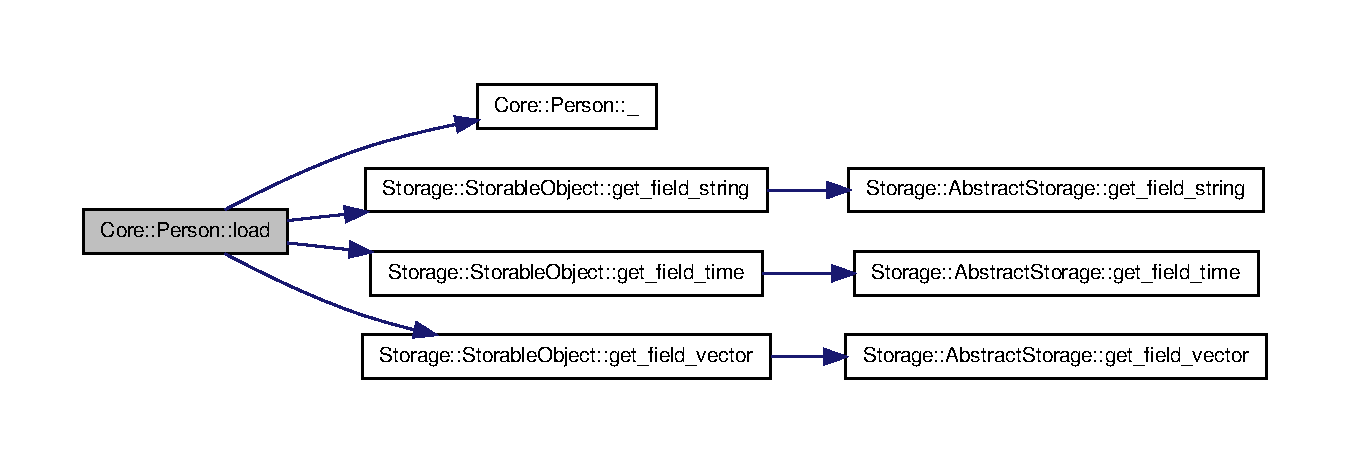
\includegraphics[width=400pt]{d9/d71/classCore_1_1Person_ae88c1b9c89b03ac7f4ba3ddcff4c62a7_cgraph}
\end{center}
\end{figure}


\hypertarget{classCore_1_1Person_a14d39111fb34383818154a26b0d248f5}{
\index{Core::Person@{Core::Person}!name@{name}}
\index{name@{name}!Core::Person@{Core::Person}}
\subsubsection[{name}]{\setlength{\rightskip}{0pt plus 5cm}const std::string Core::Person::name (
\begin{DoxyParamCaption}
{}
\end{DoxyParamCaption}
) const\hspace{0.3cm}{\ttfamily  \mbox{[}inline\mbox{]}}}}
\label{d9/d71/classCore_1_1Person_a14d39111fb34383818154a26b0d248f5}
\begin{Desc}
\item[\hyperlink{deprecated__deprecated000004}{Deprecated}]Get name of person. \end{Desc}
\begin{DoxyReturn}{Returns}
name of person. 
\end{DoxyReturn}
\hypertarget{classCore_1_1Person_a3b86cab797444527364376dad2a0c300}{
\index{Core::Person@{Core::Person}!read@{read}}
\index{read@{read}!Core::Person@{Core::Person}}
\subsubsection[{read}]{\setlength{\rightskip}{0pt plus 5cm}const std::string Person::read (
\begin{DoxyParamCaption}
{}
\end{DoxyParamCaption}
) const\hspace{0.3cm}{\ttfamily  \mbox{[}virtual\mbox{]}}}}
\label{d9/d71/classCore_1_1Person_a3b86cab797444527364376dad2a0c300}


Implements \hyperlink{classUI_1_1UsersObject_a68d5297258a2f4da4ff58f4809690db3}{UI::UsersObject}.

\hypertarget{classCore_1_1Person_a5dfa21d7b0a58e09f71e07a4298f0f62}{
\index{Core::Person@{Core::Person}!read\_\-enum@{read\_\-enum}}
\index{read\_\-enum@{read\_\-enum}!Core::Person@{Core::Person}}
\subsubsection[{read\_\-enum}]{\setlength{\rightskip}{0pt plus 5cm}const std::string Person::read\_\-enum (
\begin{DoxyParamCaption}
\item[{const std::string}]{name}
\end{DoxyParamCaption}
) const  throw (std::bad\_\-cast)\hspace{0.3cm}{\ttfamily  \mbox{[}virtual\mbox{]}}}}
\label{d9/d71/classCore_1_1Person_a5dfa21d7b0a58e09f71e07a4298f0f62}


Implements \hyperlink{classUI_1_1UsersObject_a20ea26010f60e60f38d380fdaa9240d5}{UI::UsersObject}.

\hypertarget{classCore_1_1Person_a9b1601502537f54b7c33fc593f8df590}{
\index{Core::Person@{Core::Person}!read\_\-int@{read\_\-int}}
\index{read\_\-int@{read\_\-int}!Core::Person@{Core::Person}}
\subsubsection[{read\_\-int}]{\setlength{\rightskip}{0pt plus 5cm}const int Person::read\_\-int (
\begin{DoxyParamCaption}
\item[{const std::string}]{name}
\end{DoxyParamCaption}
) const  throw (std::bad\_\-cast)\hspace{0.3cm}{\ttfamily  \mbox{[}virtual\mbox{]}}}}
\label{d9/d71/classCore_1_1Person_a9b1601502537f54b7c33fc593f8df590}


Implements \hyperlink{classUI_1_1UsersObject_a63ab79bb54b6134a483b2e384c824c7e}{UI::UsersObject}.

\hypertarget{classCore_1_1Person_a4b7d0b1c545c2c4876b3f410b914f3a2}{
\index{Core::Person@{Core::Person}!read\_\-string@{read\_\-string}}
\index{read\_\-string@{read\_\-string}!Core::Person@{Core::Person}}
\subsubsection[{read\_\-string}]{\setlength{\rightskip}{0pt plus 5cm}const std::string Person::read\_\-string (
\begin{DoxyParamCaption}
\item[{const std::string}]{name}
\end{DoxyParamCaption}
) const  throw (std::bad\_\-cast)\hspace{0.3cm}{\ttfamily  \mbox{[}virtual\mbox{]}}}}
\label{d9/d71/classCore_1_1Person_a4b7d0b1c545c2c4876b3f410b914f3a2}


Implements \hyperlink{classUI_1_1UsersObject_aed80fcf20b550a0e3484fbe6beb24c19}{UI::UsersObject}.

\hypertarget{classCore_1_1Person_ad0485ff28f4f80aeb0da9f8a6ae2f6d0}{
\index{Core::Person@{Core::Person}!read\_\-time@{read\_\-time}}
\index{read\_\-time@{read\_\-time}!Core::Person@{Core::Person}}
\subsubsection[{read\_\-time}]{\setlength{\rightskip}{0pt plus 5cm}const time\_\-t Person::read\_\-time (
\begin{DoxyParamCaption}
\item[{const std::string}]{name}
\end{DoxyParamCaption}
) const  throw (std::bad\_\-cast)\hspace{0.3cm}{\ttfamily  \mbox{[}virtual\mbox{]}}}}
\label{d9/d71/classCore_1_1Person_ad0485ff28f4f80aeb0da9f8a6ae2f6d0}


Implements \hyperlink{classUI_1_1UsersObject_a490536c477c5a796724ce26fd010c680}{UI::UsersObject}.

\hypertarget{classCore_1_1Person_ab28c3e468d265c16bce1d4488493c5a6}{
\index{Core::Person@{Core::Person}!read\_\-vector@{read\_\-vector}}
\index{read\_\-vector@{read\_\-vector}!Core::Person@{Core::Person}}
\subsubsection[{read\_\-vector}]{\setlength{\rightskip}{0pt plus 5cm}const std::vector$<$ {\bf UI::UsersObject} $\ast$ $>$ Person::read\_\-vector (
\begin{DoxyParamCaption}
\item[{const std::string}]{name}
\end{DoxyParamCaption}
) const  throw (std::bad\_\-cast)\hspace{0.3cm}{\ttfamily  \mbox{[}virtual\mbox{]}}}}
\label{d9/d71/classCore_1_1Person_ab28c3e468d265c16bce1d4488493c5a6}


Implements \hyperlink{classUI_1_1UsersObject_a6899d8a06268abb8f2a13feba9921ce5}{UI::UsersObject}.

\hypertarget{classCore_1_1Person_a846fa55a79f6da0258d711adc88a1a30}{
\index{Core::Person@{Core::Person}!save@{save}}
\index{save@{save}!Core::Person@{Core::Person}}
\subsubsection[{save}]{\setlength{\rightskip}{0pt plus 5cm}void Person::save (
\begin{DoxyParamCaption}
{}
\end{DoxyParamCaption}
)\hspace{0.3cm}{\ttfamily  \mbox{[}protected, virtual\mbox{]}}}}
\label{d9/d71/classCore_1_1Person_a846fa55a79f6da0258d711adc88a1a30}
Save all data into storage. Virtual in \hyperlink{classStorage_1_1StorableObject}{Storage::StorableObject}. 

Implements \hyperlink{classStorage_1_1StorableObject_a85609f4a18b49c7e0eed0205ee6df5d9}{Storage::StorableObject}.



Here is the call graph for this function:
\nopagebreak
\begin{figure}[H]
\begin{center}
\leavevmode
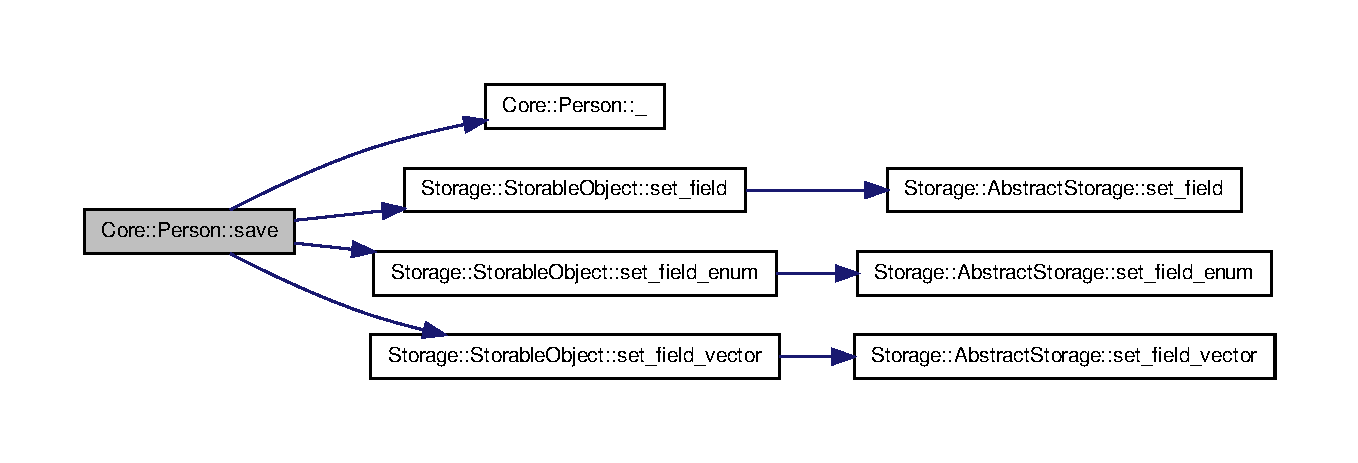
\includegraphics[width=400pt]{d9/d71/classCore_1_1Person_a846fa55a79f6da0258d711adc88a1a30_cgraph}
\end{center}
\end{figure}


\hypertarget{classCore_1_1Person_a0d70ad24edf86e3c0f88e913342aa24d}{
\index{Core::Person@{Core::Person}!sex@{sex}}
\index{sex@{sex}!Core::Person@{Core::Person}}
\subsubsection[{sex}]{\setlength{\rightskip}{0pt plus 5cm}enum {\bf Sex} Core::Person::sex (
\begin{DoxyParamCaption}
{}
\end{DoxyParamCaption}
) const\hspace{0.3cm}{\ttfamily  \mbox{[}inline\mbox{]}}}}
\label{d9/d71/classCore_1_1Person_a0d70ad24edf86e3c0f88e913342aa24d}
\begin{Desc}
\item[\hyperlink{deprecated__deprecated000006}{Deprecated}]Get sex of person. \end{Desc}
\begin{DoxyReturn}{Returns}
person's sex. 
\end{DoxyReturn}
\hypertarget{classCore_1_1Person_a5572207d53649af10cd9bb62fe21995c}{
\index{Core::Person@{Core::Person}!surname@{surname}}
\index{surname@{surname}!Core::Person@{Core::Person}}
\subsubsection[{surname}]{\setlength{\rightskip}{0pt plus 5cm}const std::string Core::Person::surname (
\begin{DoxyParamCaption}
{}
\end{DoxyParamCaption}
) const\hspace{0.3cm}{\ttfamily  \mbox{[}inline\mbox{]}}}}
\label{d9/d71/classCore_1_1Person_a5572207d53649af10cd9bb62fe21995c}
\begin{Desc}
\item[\hyperlink{deprecated__deprecated000005}{Deprecated}]Get surname of person. \end{Desc}
\begin{DoxyReturn}{Returns}
surname of person. 
\end{DoxyReturn}
\hypertarget{classCore_1_1Person_ac2900dc24258c00ea1de17350c3f4658}{
\index{Core::Person@{Core::Person}!update@{update}}
\index{update@{update}!Core::Person@{Core::Person}}
\subsubsection[{update}]{\setlength{\rightskip}{0pt plus 5cm}void Person::update (
\begin{DoxyParamCaption}
\item[{const std::string}]{name, }
\item[{const int}]{value}
\end{DoxyParamCaption}
)  throw (std::bad\_\-cast)\hspace{0.3cm}{\ttfamily  \mbox{[}virtual\mbox{]}}}}
\label{d9/d71/classCore_1_1Person_ac2900dc24258c00ea1de17350c3f4658}


Implements \hyperlink{classUI_1_1UsersObject_a9b30123c0a25a66715bce9a58a27d37e}{UI::UsersObject}.

\hypertarget{classCore_1_1Person_a51ec02307587cf9dfd7ed3036cf202cd}{
\index{Core::Person@{Core::Person}!update@{update}}
\index{update@{update}!Core::Person@{Core::Person}}
\subsubsection[{update}]{\setlength{\rightskip}{0pt plus 5cm}void Person::update (
\begin{DoxyParamCaption}
\item[{const std::string}]{name, }
\item[{const std::string}]{value}
\end{DoxyParamCaption}
)  throw (std::bad\_\-cast)\hspace{0.3cm}{\ttfamily  \mbox{[}virtual\mbox{]}}}}
\label{d9/d71/classCore_1_1Person_a51ec02307587cf9dfd7ed3036cf202cd}


Implements \hyperlink{classUI_1_1UsersObject_a4c86312e8400ce3e1b5d2c17552ce5f5}{UI::UsersObject}.

\hypertarget{classCore_1_1Person_ad650eba89f671041c26f8d1419f6e6c8}{
\index{Core::Person@{Core::Person}!update@{update}}
\index{update@{update}!Core::Person@{Core::Person}}
\subsubsection[{update}]{\setlength{\rightskip}{0pt plus 5cm}void Person::update (
\begin{DoxyParamCaption}
\item[{const std::string}]{name, }
\item[{const time\_\-t}]{value}
\end{DoxyParamCaption}
)  throw (std::bad\_\-cast)\hspace{0.3cm}{\ttfamily  \mbox{[}virtual\mbox{]}}}}
\label{d9/d71/classCore_1_1Person_ad650eba89f671041c26f8d1419f6e6c8}


Implements \hyperlink{classUI_1_1UsersObject_add0bfcc5674bd3f56eeb68919c640bb7}{UI::UsersObject}.

\hypertarget{classCore_1_1Person_a50fa1e127f56e2caa873017b54c090cb}{
\index{Core::Person@{Core::Person}!update@{update}}
\index{update@{update}!Core::Person@{Core::Person}}
\subsubsection[{update}]{\setlength{\rightskip}{0pt plus 5cm}virtual void Core::Person::update (
\begin{DoxyParamCaption}
\item[{UsersObject $\ast$}]{, }
\item[{bool}]{linked}
\end{DoxyParamCaption}
)  throw (std::bad\_\-cast)\hspace{0.3cm}{\ttfamily  \mbox{[}virtual\mbox{]}}}}
\label{d9/d71/classCore_1_1Person_a50fa1e127f56e2caa873017b54c090cb}
\hypertarget{classCore_1_1Person_a1c6826659c2413189dae536f7c83af98}{
\index{Core::Person@{Core::Person}!update\_\-enum@{update\_\-enum}}
\index{update\_\-enum@{update\_\-enum}!Core::Person@{Core::Person}}
\subsubsection[{update\_\-enum}]{\setlength{\rightskip}{0pt plus 5cm}void Person::update\_\-enum (
\begin{DoxyParamCaption}
\item[{const std::string}]{name, }
\item[{const std::string}]{value}
\end{DoxyParamCaption}
)  throw (std::bad\_\-cast)\hspace{0.3cm}{\ttfamily  \mbox{[}virtual\mbox{]}}}}
\label{d9/d71/classCore_1_1Person_a1c6826659c2413189dae536f7c83af98}


Implements \hyperlink{classUI_1_1UsersObject_a925f50c5cb5123a13493f76029ae6f06}{UI::UsersObject}.



\subsection{Friends And Related Function Documentation}
\hypertarget{classCore_1_1Person_a8be971ab18693e55f617c7dc8abc3e26}{
\index{Core::Person@{Core::Person}!AbstractGroup@{AbstractGroup}}
\index{AbstractGroup@{AbstractGroup}!Core::Person@{Core::Person}}
\subsubsection[{AbstractGroup}]{\setlength{\rightskip}{0pt plus 5cm}friend class {\bf AbstractGroup}\hspace{0.3cm}{\ttfamily  \mbox{[}friend\mbox{]}}}}
\label{d9/d71/classCore_1_1Person_a8be971ab18693e55f617c7dc8abc3e26}


The documentation for this class was generated from the following files:\begin{DoxyCompactItemize}
\item 
src/include/\hyperlink{person_8h}{person.h}\item 
src/core/\hyperlink{person_8cpp}{person.cpp}\end{DoxyCompactItemize}

\hypertarget{classSQLiteStorage}{
\section{SQLiteStorage Class Reference}
\label{db/d2a/classSQLiteStorage}\index{SQLiteStorage@{SQLiteStorage}}
}


Inheritance diagram for SQLiteStorage:
\nopagebreak
\begin{figure}[H]
\begin{center}
\leavevmode
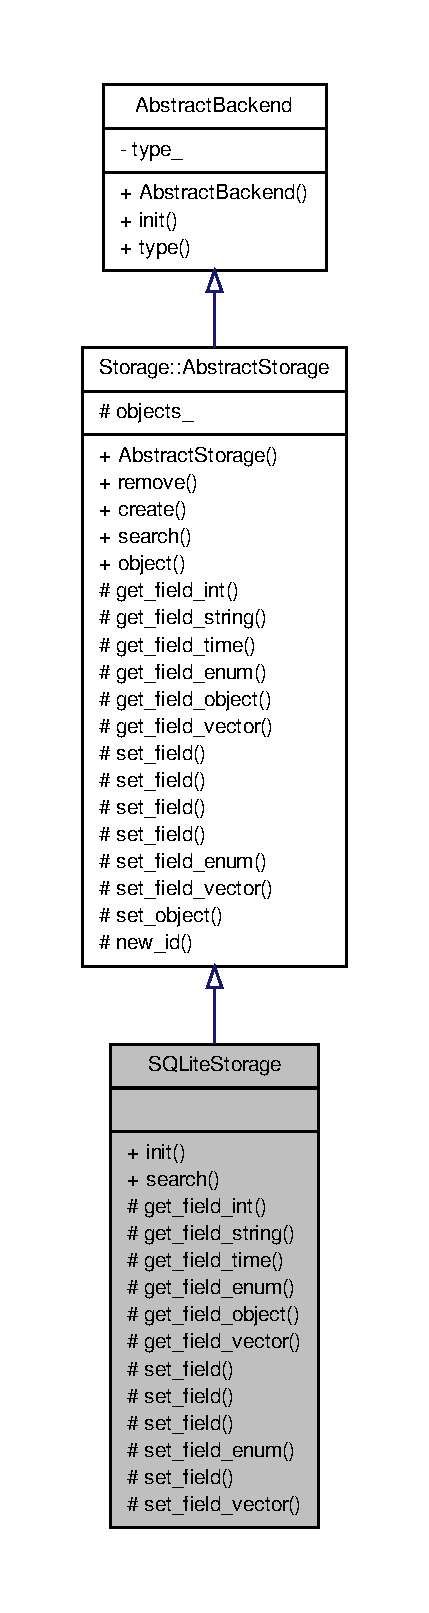
\includegraphics[height=600pt]{d1/d14/classSQLiteStorage__inherit__graph}
\end{center}
\end{figure}


Collaboration diagram for SQLiteStorage:
\nopagebreak
\begin{figure}[H]
\begin{center}
\leavevmode
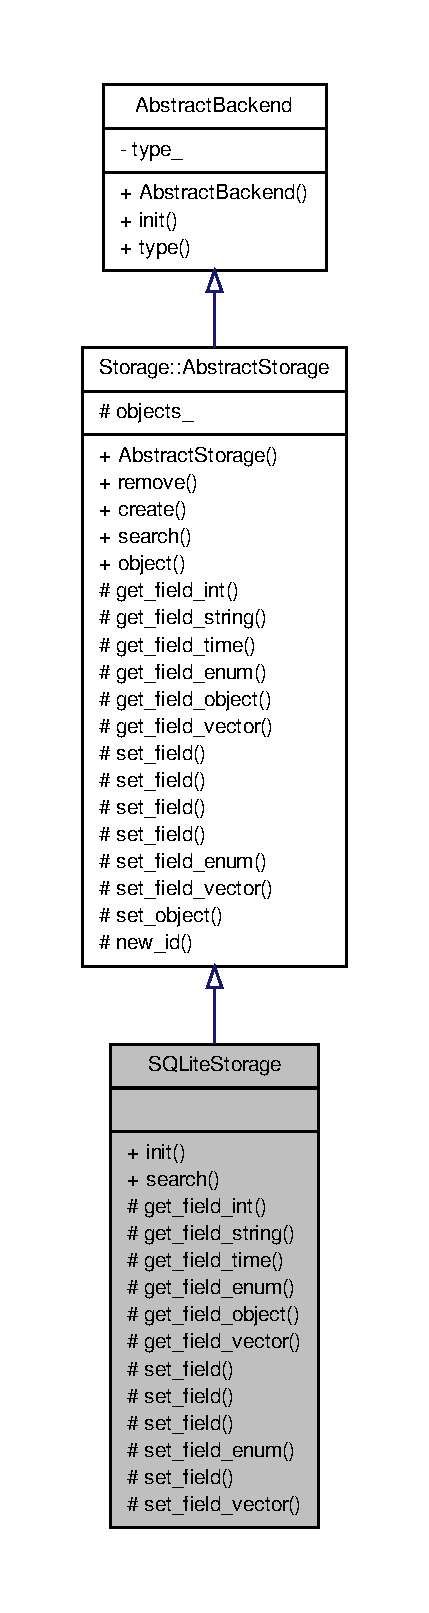
\includegraphics[height=600pt]{d3/dc2/classSQLiteStorage__coll__graph}
\end{center}
\end{figure}
\subsection*{Public Member Functions}
\begin{DoxyCompactItemize}
\item 
virtual void \hyperlink{classSQLiteStorage_a1abd27f3824567fef222479a7c7a2333}{init} (const std::vector$<$ std::string $>$ \&args)
\item 
virtual std::vector$<$ \hyperlink{classStorage_1_1StorableObject}{Storage::StorableObject} $\ast$ $>$ $\ast$ \hyperlink{classSQLiteStorage_ae3b74f8ac83d9f0c9d5cadc66daab68e}{search} (std::vector$<$ \hyperlink{structStorage_1_1AbstractStorage_1_1Argument}{Storage::AbstractStorage::Argument} $\ast$ $>$ \&args)
\end{DoxyCompactItemize}
\subsection*{Protected Member Functions}
\begin{DoxyCompactItemize}
\item 
virtual const int \hyperlink{classSQLiteStorage_aab5d70b4dbe29dbe6e9243a89ee81a89}{get\_\-field\_\-int} (const int id, const std::string name) const   throw (std::bad\_\-cast)
\begin{DoxyCompactList}\small\item\em Return integer value of requested field. \item\end{DoxyCompactList}\item 
virtual const std::string \hyperlink{classSQLiteStorage_a5a68da392583ef992a3aff78cfdacc8a}{get\_\-field\_\-string} (const int id, const std::string name) const   throw (std::bad\_\-cast)
\begin{DoxyCompactList}\small\item\em Return string value of requested field. \item\end{DoxyCompactList}\item 
virtual const time\_\-t \hyperlink{classSQLiteStorage_a5fe9e128b183bea0ee7f046eba38cedd}{get\_\-field\_\-time} (const int id, const std::string name) const   throw (std::bad\_\-cast)
\begin{DoxyCompactList}\small\item\em Return time value of requested field. \item\end{DoxyCompactList}\item 
virtual const std::string \hyperlink{classSQLiteStorage_aef325b647f98c8e5fdb402ec608b403b}{get\_\-field\_\-enum} (const int id, const std::string name) const   throw (std::bad\_\-cast)
\begin{DoxyCompactList}\small\item\em Return enum value of requested field. \item\end{DoxyCompactList}\item 
virtual \hyperlink{classStorage_1_1StorableObject}{Storage::StorableObject} $\ast$ \hyperlink{classSQLiteStorage_adf1189839ae893f3ce4c73c3ee69634d}{get\_\-field\_\-object} (const int id, const std::string name) const   throw (std::bad\_\-cast)
\begin{DoxyCompactList}\small\item\em Return object value of requested field. \item\end{DoxyCompactList}\item 
virtual const std::vector$<$ \hyperlink{classStorage_1_1StorableObject}{Storage::StorableObject} $\ast$ $>$ \hyperlink{classSQLiteStorage_a818cc8edbbe849eabacbdc055a32ad6a}{get\_\-field\_\-vector} (const int id, const std::string name) const   throw (std::bad\_\-cast)
\begin{DoxyCompactList}\small\item\em Return vector value of requested field. \item\end{DoxyCompactList}\item 
virtual void \hyperlink{classSQLiteStorage_a3e1271c2699a0e5a82452a21e5d1af63}{set\_\-field} (const int id, const std::string name, const int value)  throw (std::bad\_\-cast)
\begin{DoxyCompactList}\small\item\em Set integer value of requested field. \item\end{DoxyCompactList}\item 
virtual void \hyperlink{classSQLiteStorage_ac353c289df54fce5f5658746824fcbac}{set\_\-field} (const int id, const std::string name, const std::string value)  throw (std::bad\_\-cast)
\begin{DoxyCompactList}\small\item\em Set string value of requested field. \item\end{DoxyCompactList}\item 
virtual void \hyperlink{classSQLiteStorage_a36665e18b5290da4c7bab56d22703d03}{set\_\-field} (const int id, const std::string name, const time\_\-t value)  throw (std::bad\_\-cast)
\begin{DoxyCompactList}\small\item\em Set time value of requested field. \item\end{DoxyCompactList}\item 
virtual void \hyperlink{classSQLiteStorage_a1b8a3f2ad138447ad5815e857eea333e}{set\_\-field\_\-enum} (const int id, const std::string name, const std::string value)  throw (std::bad\_\-cast)
\begin{DoxyCompactList}\small\item\em Set enum value of requested field. \item\end{DoxyCompactList}\item 
virtual void \hyperlink{classSQLiteStorage_ab2b3d9fcde8dbcd28eb66f60a6cf13ac}{set\_\-field} (const int id, const std::string name, \hyperlink{classStorage_1_1StorableObject}{Storage::StorableObject} $\ast$value)  throw (std::bad\_\-cast)
\begin{DoxyCompactList}\small\item\em Set object value of requested field. \item\end{DoxyCompactList}\item 
virtual void \hyperlink{classSQLiteStorage_a41c576c779146896a0cd0b18228a643e}{set\_\-field\_\-vector} (const int id, const std::string name, const std::vector$<$ \hyperlink{classStorage_1_1StorableObject}{Storage::StorableObject} $\ast$ $>$ value)  throw (std::bad\_\-cast)
\begin{DoxyCompactList}\small\item\em Set vector value of requested field. \item\end{DoxyCompactList}\end{DoxyCompactItemize}


\subsection{Member Function Documentation}
\hypertarget{classSQLiteStorage_aef325b647f98c8e5fdb402ec608b403b}{
\index{SQLiteStorage@{SQLiteStorage}!get\_\-field\_\-enum@{get\_\-field\_\-enum}}
\index{get\_\-field\_\-enum@{get\_\-field\_\-enum}!SQLiteStorage@{SQLiteStorage}}
\subsubsection[{get\_\-field\_\-enum}]{\setlength{\rightskip}{0pt plus 5cm}const std::string SQLiteStorage::get\_\-field\_\-enum (
\begin{DoxyParamCaption}
\item[{const int}]{id, }
\item[{const std::string}]{field}
\end{DoxyParamCaption}
) const  throw (std::bad\_\-cast)\hspace{0.3cm}{\ttfamily  \mbox{[}protected, virtual\mbox{]}}}}
\label{db/d2a/classSQLiteStorage_aef325b647f98c8e5fdb402ec608b403b}


Return enum value of requested field. 


\begin{DoxyParams}[1]{Parameters}
\mbox{\tt in}  & {\em id} & Object identificator. \\
\hline
\mbox{\tt in}  & {\em field} & Field name. \\
\hline
\end{DoxyParams}
\begin{DoxyReturn}{Returns}
requested value.
\end{DoxyReturn}
This method must be realized in inherited classes. Throw an std::bad\_\-cast exception if requested field does not exists or keeped in another type. 

Implements \hyperlink{classStorage_1_1AbstractStorage_acd7e88a005b6873632c7f20245e5f3f7}{Storage::AbstractStorage}.

\hypertarget{classSQLiteStorage_aab5d70b4dbe29dbe6e9243a89ee81a89}{
\index{SQLiteStorage@{SQLiteStorage}!get\_\-field\_\-int@{get\_\-field\_\-int}}
\index{get\_\-field\_\-int@{get\_\-field\_\-int}!SQLiteStorage@{SQLiteStorage}}
\subsubsection[{get\_\-field\_\-int}]{\setlength{\rightskip}{0pt plus 5cm}const int SQLiteStorage::get\_\-field\_\-int (
\begin{DoxyParamCaption}
\item[{const int}]{id, }
\item[{const std::string}]{field}
\end{DoxyParamCaption}
) const  throw (std::bad\_\-cast)\hspace{0.3cm}{\ttfamily  \mbox{[}protected, virtual\mbox{]}}}}
\label{db/d2a/classSQLiteStorage_aab5d70b4dbe29dbe6e9243a89ee81a89}


Return integer value of requested field. 


\begin{DoxyParams}[1]{Parameters}
\mbox{\tt in}  & {\em id} & Object identificator. \\
\hline
\mbox{\tt in}  & {\em field} & Field name. \\
\hline
\end{DoxyParams}
\begin{DoxyReturn}{Returns}
requested value.
\end{DoxyReturn}
This method must be realized in inherited classes. Throw an std::bad\_\-cast exception if requested field does not exists or keeped in another type. 

Implements \hyperlink{classStorage_1_1AbstractStorage_a80a7e4ab87a0326aa8b5571b09d55eaa}{Storage::AbstractStorage}.

\hypertarget{classSQLiteStorage_adf1189839ae893f3ce4c73c3ee69634d}{
\index{SQLiteStorage@{SQLiteStorage}!get\_\-field\_\-object@{get\_\-field\_\-object}}
\index{get\_\-field\_\-object@{get\_\-field\_\-object}!SQLiteStorage@{SQLiteStorage}}
\subsubsection[{get\_\-field\_\-object}]{\setlength{\rightskip}{0pt plus 5cm}{\bf Storage::StorableObject} $\ast$ SQLiteStorage::get\_\-field\_\-object (
\begin{DoxyParamCaption}
\item[{const int}]{id, }
\item[{const std::string}]{field}
\end{DoxyParamCaption}
) const  throw (std::bad\_\-cast)\hspace{0.3cm}{\ttfamily  \mbox{[}protected, virtual\mbox{]}}}}
\label{db/d2a/classSQLiteStorage_adf1189839ae893f3ce4c73c3ee69634d}


Return object value of requested field. 


\begin{DoxyParams}[1]{Parameters}
\mbox{\tt in}  & {\em id} & Object identificator. \\
\hline
\mbox{\tt in}  & {\em field} & Field name. \\
\hline
\end{DoxyParams}
\begin{DoxyReturn}{Returns}
requested value.
\end{DoxyReturn}
This method must be realized in inherited classes. Throw an std::bad\_\-cast exception if requested field does not exists or keeped in another type. 

Implements \hyperlink{classStorage_1_1AbstractStorage_aaff107d1f51e456f26c03861beb0fff7}{Storage::AbstractStorage}.

\hypertarget{classSQLiteStorage_a5a68da392583ef992a3aff78cfdacc8a}{
\index{SQLiteStorage@{SQLiteStorage}!get\_\-field\_\-string@{get\_\-field\_\-string}}
\index{get\_\-field\_\-string@{get\_\-field\_\-string}!SQLiteStorage@{SQLiteStorage}}
\subsubsection[{get\_\-field\_\-string}]{\setlength{\rightskip}{0pt plus 5cm}const std::string SQLiteStorage::get\_\-field\_\-string (
\begin{DoxyParamCaption}
\item[{const int}]{id, }
\item[{const std::string}]{field}
\end{DoxyParamCaption}
) const  throw (std::bad\_\-cast)\hspace{0.3cm}{\ttfamily  \mbox{[}protected, virtual\mbox{]}}}}
\label{db/d2a/classSQLiteStorage_a5a68da392583ef992a3aff78cfdacc8a}


Return string value of requested field. 


\begin{DoxyParams}[1]{Parameters}
\mbox{\tt in}  & {\em id} & Object identificator. \\
\hline
\mbox{\tt in}  & {\em field} & Field name. \\
\hline
\end{DoxyParams}
\begin{DoxyReturn}{Returns}
requested value.
\end{DoxyReturn}
This method must be realized in inherited classes. Throw an std::bad\_\-cast exception if requested field does not exists or keeped in another type. 

Implements \hyperlink{classStorage_1_1AbstractStorage_ad12a3abb791ef5a696196c28e643ec22}{Storage::AbstractStorage}.

\hypertarget{classSQLiteStorage_a5fe9e128b183bea0ee7f046eba38cedd}{
\index{SQLiteStorage@{SQLiteStorage}!get\_\-field\_\-time@{get\_\-field\_\-time}}
\index{get\_\-field\_\-time@{get\_\-field\_\-time}!SQLiteStorage@{SQLiteStorage}}
\subsubsection[{get\_\-field\_\-time}]{\setlength{\rightskip}{0pt plus 5cm}const time\_\-t SQLiteStorage::get\_\-field\_\-time (
\begin{DoxyParamCaption}
\item[{const int}]{id, }
\item[{const std::string}]{field}
\end{DoxyParamCaption}
) const  throw (std::bad\_\-cast)\hspace{0.3cm}{\ttfamily  \mbox{[}protected, virtual\mbox{]}}}}
\label{db/d2a/classSQLiteStorage_a5fe9e128b183bea0ee7f046eba38cedd}


Return time value of requested field. 


\begin{DoxyParams}[1]{Parameters}
\mbox{\tt in}  & {\em id} & Object identificator. \\
\hline
\mbox{\tt in}  & {\em field} & Field name. \\
\hline
\end{DoxyParams}
\begin{DoxyReturn}{Returns}
requested value.
\end{DoxyReturn}
This method must be realized in inherited classes. Throw an std::bad\_\-cast exception if requested field does not exists or keeped in another type. 

Implements \hyperlink{classStorage_1_1AbstractStorage_a87fe8d51934ab2403758d905ef313272}{Storage::AbstractStorage}.

\hypertarget{classSQLiteStorage_a818cc8edbbe849eabacbdc055a32ad6a}{
\index{SQLiteStorage@{SQLiteStorage}!get\_\-field\_\-vector@{get\_\-field\_\-vector}}
\index{get\_\-field\_\-vector@{get\_\-field\_\-vector}!SQLiteStorage@{SQLiteStorage}}
\subsubsection[{get\_\-field\_\-vector}]{\setlength{\rightskip}{0pt plus 5cm}const std::vector$<$ {\bf Storage::StorableObject} $\ast$ $>$ SQLiteStorage::get\_\-field\_\-vector (
\begin{DoxyParamCaption}
\item[{const int}]{id, }
\item[{const std::string}]{field}
\end{DoxyParamCaption}
) const  throw (std::bad\_\-cast)\hspace{0.3cm}{\ttfamily  \mbox{[}protected, virtual\mbox{]}}}}
\label{db/d2a/classSQLiteStorage_a818cc8edbbe849eabacbdc055a32ad6a}


Return vector value of requested field. 


\begin{DoxyParams}[1]{Parameters}
\mbox{\tt in}  & {\em id} & Object identificator. \\
\hline
\mbox{\tt in}  & {\em field} & Field name. \\
\hline
\end{DoxyParams}
\begin{DoxyReturn}{Returns}
requested value.
\end{DoxyReturn}
This method must be realized in inherited classes. Throw an std::bad\_\-cast exception if requested field does not exists or keeped in another type. 

Implements \hyperlink{classStorage_1_1AbstractStorage_ae7c30697d68dc9d7de595388030d8e10}{Storage::AbstractStorage}.

\hypertarget{classSQLiteStorage_a1abd27f3824567fef222479a7c7a2333}{
\index{SQLiteStorage@{SQLiteStorage}!init@{init}}
\index{init@{init}!SQLiteStorage@{SQLiteStorage}}
\subsubsection[{init}]{\setlength{\rightskip}{0pt plus 5cm}void SQLiteStorage::init (
\begin{DoxyParamCaption}
\item[{const std::vector$<$ std::string $>$ \&}]{args}
\end{DoxyParamCaption}
)\hspace{0.3cm}{\ttfamily  \mbox{[}virtual\mbox{]}}}}
\label{db/d2a/classSQLiteStorage_a1abd27f3824567fef222479a7c7a2333}


Implements \hyperlink{classAbstractBackend_afce49841a79e3093a1fbf199bfd9f698}{AbstractBackend}.

\hypertarget{classSQLiteStorage_ae3b74f8ac83d9f0c9d5cadc66daab68e}{
\index{SQLiteStorage@{SQLiteStorage}!search@{search}}
\index{search@{search}!SQLiteStorage@{SQLiteStorage}}
\subsubsection[{search}]{\setlength{\rightskip}{0pt plus 5cm}std::vector$<$ {\bf Storage::StorableObject} $\ast$ $>$ $\ast$ SQLiteStorage::search (
\begin{DoxyParamCaption}
\item[{std::vector$<$ {\bf Storage::AbstractStorage::Argument} $\ast$ $>$ \&}]{args}
\end{DoxyParamCaption}
)\hspace{0.3cm}{\ttfamily  \mbox{[}virtual\mbox{]}}}}
\label{db/d2a/classSQLiteStorage_ae3b74f8ac83d9f0c9d5cadc66daab68e}
\hypertarget{classSQLiteStorage_a36665e18b5290da4c7bab56d22703d03}{
\index{SQLiteStorage@{SQLiteStorage}!set\_\-field@{set\_\-field}}
\index{set\_\-field@{set\_\-field}!SQLiteStorage@{SQLiteStorage}}
\subsubsection[{set\_\-field}]{\setlength{\rightskip}{0pt plus 5cm}void SQLiteStorage::set\_\-field (
\begin{DoxyParamCaption}
\item[{const int}]{id, }
\item[{const std::string}]{field, }
\item[{const time\_\-t}]{value}
\end{DoxyParamCaption}
)  throw (std::bad\_\-cast)\hspace{0.3cm}{\ttfamily  \mbox{[}protected, virtual\mbox{]}}}}
\label{db/d2a/classSQLiteStorage_a36665e18b5290da4c7bab56d22703d03}


Set time value of requested field. 


\begin{DoxyParams}[1]{Parameters}
\mbox{\tt in}  & {\em id} & Object identificator. \\
\hline
\mbox{\tt in}  & {\em field} & Field name. \\
\hline
\mbox{\tt in}  & {\em value} & New value.\\
\hline
\end{DoxyParams}
This method must be realized in inherited classes. Throw an std::bad\_\-cast exception if requested field keeped in another type. 

Implements \hyperlink{classStorage_1_1AbstractStorage_a50ee4a829bc067a9291a11aa99ec0f16}{Storage::AbstractStorage}.

\hypertarget{classSQLiteStorage_ac353c289df54fce5f5658746824fcbac}{
\index{SQLiteStorage@{SQLiteStorage}!set\_\-field@{set\_\-field}}
\index{set\_\-field@{set\_\-field}!SQLiteStorage@{SQLiteStorage}}
\subsubsection[{set\_\-field}]{\setlength{\rightskip}{0pt plus 5cm}void SQLiteStorage::set\_\-field (
\begin{DoxyParamCaption}
\item[{const int}]{id, }
\item[{const std::string}]{field, }
\item[{const std::string}]{value}
\end{DoxyParamCaption}
)  throw (std::bad\_\-cast)\hspace{0.3cm}{\ttfamily  \mbox{[}protected, virtual\mbox{]}}}}
\label{db/d2a/classSQLiteStorage_ac353c289df54fce5f5658746824fcbac}


Set string value of requested field. 


\begin{DoxyParams}[1]{Parameters}
\mbox{\tt in}  & {\em id} & Object identificator. \\
\hline
\mbox{\tt in}  & {\em field} & Field name. \\
\hline
\mbox{\tt in}  & {\em value} & New value.\\
\hline
\end{DoxyParams}
This method must be realized in inherited classes. Throw an std::bad\_\-cast exception if requested field keeped in another type. 

Implements \hyperlink{classStorage_1_1AbstractStorage_ae5ee00e647f121b68ebada0f094058bc}{Storage::AbstractStorage}.

\hypertarget{classSQLiteStorage_a3e1271c2699a0e5a82452a21e5d1af63}{
\index{SQLiteStorage@{SQLiteStorage}!set\_\-field@{set\_\-field}}
\index{set\_\-field@{set\_\-field}!SQLiteStorage@{SQLiteStorage}}
\subsubsection[{set\_\-field}]{\setlength{\rightskip}{0pt plus 5cm}void SQLiteStorage::set\_\-field (
\begin{DoxyParamCaption}
\item[{const int}]{id, }
\item[{const std::string}]{field, }
\item[{const int}]{value}
\end{DoxyParamCaption}
)  throw (std::bad\_\-cast)\hspace{0.3cm}{\ttfamily  \mbox{[}protected, virtual\mbox{]}}}}
\label{db/d2a/classSQLiteStorage_a3e1271c2699a0e5a82452a21e5d1af63}


Set integer value of requested field. 


\begin{DoxyParams}[1]{Parameters}
\mbox{\tt in}  & {\em id} & Object identificator. \\
\hline
\mbox{\tt in}  & {\em field} & Field name. \\
\hline
\mbox{\tt in}  & {\em value} & New value.\\
\hline
\end{DoxyParams}
This method must be realized in inherited classes. Throw an std::bad\_\-cast exception if requested field keeped in another type. 

Implements \hyperlink{classStorage_1_1AbstractStorage_acdd090d0beb6a8241914e7d78a7f2c0c}{Storage::AbstractStorage}.

\hypertarget{classSQLiteStorage_ab2b3d9fcde8dbcd28eb66f60a6cf13ac}{
\index{SQLiteStorage@{SQLiteStorage}!set\_\-field@{set\_\-field}}
\index{set\_\-field@{set\_\-field}!SQLiteStorage@{SQLiteStorage}}
\subsubsection[{set\_\-field}]{\setlength{\rightskip}{0pt plus 5cm}void SQLiteStorage::set\_\-field (
\begin{DoxyParamCaption}
\item[{const int}]{id, }
\item[{const std::string}]{field, }
\item[{{\bf Storage::StorableObject} $\ast$}]{value}
\end{DoxyParamCaption}
)  throw (std::bad\_\-cast)\hspace{0.3cm}{\ttfamily  \mbox{[}protected, virtual\mbox{]}}}}
\label{db/d2a/classSQLiteStorage_ab2b3d9fcde8dbcd28eb66f60a6cf13ac}


Set object value of requested field. 


\begin{DoxyParams}[1]{Parameters}
\mbox{\tt in}  & {\em id} & Object identificator. \\
\hline
\mbox{\tt in}  & {\em field} & Field name. \\
\hline
\mbox{\tt in}  & {\em value} & New value.\\
\hline
\end{DoxyParams}
This method must be realized in inherited classes. Throw an std::bad\_\-cast exception if requested field keeped in another type. 

Implements \hyperlink{classStorage_1_1AbstractStorage_a7ef9f70b3fcbaa2863de2be695dc77c1}{Storage::AbstractStorage}.

\hypertarget{classSQLiteStorage_a1b8a3f2ad138447ad5815e857eea333e}{
\index{SQLiteStorage@{SQLiteStorage}!set\_\-field\_\-enum@{set\_\-field\_\-enum}}
\index{set\_\-field\_\-enum@{set\_\-field\_\-enum}!SQLiteStorage@{SQLiteStorage}}
\subsubsection[{set\_\-field\_\-enum}]{\setlength{\rightskip}{0pt plus 5cm}void SQLiteStorage::set\_\-field\_\-enum (
\begin{DoxyParamCaption}
\item[{const int}]{id, }
\item[{const std::string}]{field, }
\item[{const std::string}]{value}
\end{DoxyParamCaption}
)  throw (std::bad\_\-cast)\hspace{0.3cm}{\ttfamily  \mbox{[}protected, virtual\mbox{]}}}}
\label{db/d2a/classSQLiteStorage_a1b8a3f2ad138447ad5815e857eea333e}


Set enum value of requested field. 


\begin{DoxyParams}[1]{Parameters}
\mbox{\tt in}  & {\em id} & Object identificator. \\
\hline
\mbox{\tt in}  & {\em field} & Field name. \\
\hline
\mbox{\tt in}  & {\em value} & New value.\\
\hline
\end{DoxyParams}
This method must be realized in inherited classes. Throw an std::bad\_\-cast exception if requested field keeped in another type. 

Implements \hyperlink{classStorage_1_1AbstractStorage_a50925678c74c09acd8549a541fdbbe9f}{Storage::AbstractStorage}.

\hypertarget{classSQLiteStorage_a41c576c779146896a0cd0b18228a643e}{
\index{SQLiteStorage@{SQLiteStorage}!set\_\-field\_\-vector@{set\_\-field\_\-vector}}
\index{set\_\-field\_\-vector@{set\_\-field\_\-vector}!SQLiteStorage@{SQLiteStorage}}
\subsubsection[{set\_\-field\_\-vector}]{\setlength{\rightskip}{0pt plus 5cm}void SQLiteStorage::set\_\-field\_\-vector (
\begin{DoxyParamCaption}
\item[{const int}]{id, }
\item[{const std::string}]{field, }
\item[{const std::vector$<$ {\bf Storage::StorableObject} $\ast$ $>$}]{vector}
\end{DoxyParamCaption}
)  throw (std::bad\_\-cast)\hspace{0.3cm}{\ttfamily  \mbox{[}protected, virtual\mbox{]}}}}
\label{db/d2a/classSQLiteStorage_a41c576c779146896a0cd0b18228a643e}


Set vector value of requested field. 


\begin{DoxyParams}[1]{Parameters}
\mbox{\tt in}  & {\em id} & Object identificator. \\
\hline
\mbox{\tt in}  & {\em field} & Field name.  \mbox{[}in\mbox{]} value New value.\\
\hline
\end{DoxyParams}
This method must be realized in inherited classes. Throw an std::bad\_\-cast exception if requested field keeped in another type. 

Implements \hyperlink{classStorage_1_1AbstractStorage_a24af03b9a68ace199b0a6fa812abad39}{Storage::AbstractStorage}.



The documentation for this class was generated from the following file:\begin{DoxyCompactItemize}
\item 
src/backends/storage/\hyperlink{sqlite_8cpp}{sqlite.cpp}\end{DoxyCompactItemize}

\hypertarget{classStorage_1_1StorableObject}{
\section{Storage::StorableObject Class Reference}
\label{d4/deb/classStorage_1_1StorableObject}\index{Storage::StorableObject@{Storage::StorableObject}}
}


{\ttfamily \#include $<$storableobject.h$>$}

Inheritance diagram for Storage::StorableObject:\begin{figure}[H]
\begin{center}
\leavevmode
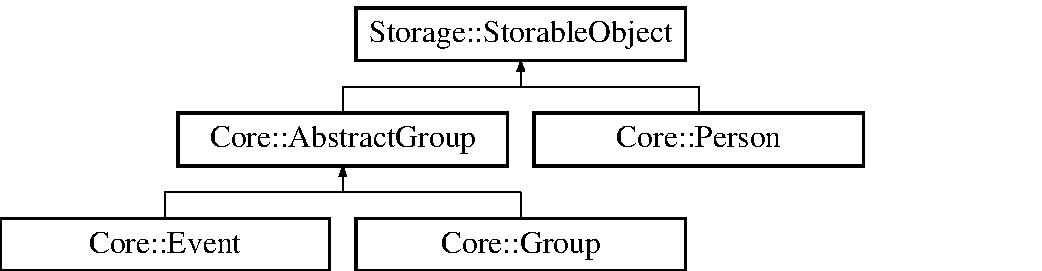
\includegraphics[height=3.000000cm]{d4/deb/classStorage_1_1StorableObject}
\end{center}
\end{figure}
\subsection*{Public Member Functions}
\begin{DoxyCompactItemize}
\item 
\hyperlink{classStorage_1_1StorableObject_ac55bb0a7b94a98ff8f14e4164150ecb0}{StorableObject} (const int id, \hyperlink{classStorage_1_1AbstractStorage}{AbstractStorage} \&storage)
\end{DoxyCompactItemize}
\subsection*{Protected Member Functions}
\begin{DoxyCompactItemize}
\item 
const int \hyperlink{classStorage_1_1StorableObject_ae3e389b184651f78594df7f83f944a2c}{id} () const 
\item 
const int \hyperlink{classStorage_1_1StorableObject_a11a172f37f8805453225be4fa98e87ae}{get\_\-field\_\-int} (const std::string name) const 
\item 
const std::string \hyperlink{classStorage_1_1StorableObject_a533b48a050009b86e376269e886d3eeb}{get\_\-field\_\-string} (const std::string name) const 
\item 
const time\_\-t \hyperlink{classStorage_1_1StorableObject_a8c4e071ed59d2cdd5d2a00806211b4e1}{get\_\-field\_\-time} (const std::string name) const 
\item 
const std::string \hyperlink{classStorage_1_1StorableObject_abcaf10bdc0f2db297c53cbd9ca0acd4d}{get\_\-field\_\-enum} (const std::string name) const 
\item 
const \hyperlink{classStorage_1_1StorableObject}{StorableObject} \& \hyperlink{classStorage_1_1StorableObject_a1f48a3363218ebfe985149b33d072067}{get\_\-field\_\-object} (const std::string name) const 
\item 
std::vector$<$ \hyperlink{classStorage_1_1StorableObject}{StorableObject} $\ast$ $>$ \hyperlink{classStorage_1_1StorableObject_ad6df389823d8f812e4c64994d440475b}{get\_\-field\_\-vector} (const std::string name) const 
\item 
void \hyperlink{classStorage_1_1StorableObject_a4c15433a6719f4036705d989828e4933}{set\_\-field} (const std::string name, const int value)
\item 
void \hyperlink{classStorage_1_1StorableObject_a95c8d3440fa0ef6bce0f8d3bbac1f477}{set\_\-field} (const std::string name, const std::string value)
\item 
void \hyperlink{classStorage_1_1StorableObject_af16a9fb211fd421a5aa89d741a67c2fb}{set\_\-field} (const std::string name, const time\_\-t value)
\item 
void \hyperlink{classStorage_1_1StorableObject_a14764d884ae0cfc51aab3c391423f781}{set\_\-field\_\-enum} (const std::string name, const std::string)
\item 
void \hyperlink{classStorage_1_1StorableObject_a97dd82cb4f99d421e84e3bac17dc8c8b}{set\_\-field} (const std::string name, const \hyperlink{classStorage_1_1StorableObject}{StorableObject} \&value)
\item 
void \hyperlink{classStorage_1_1StorableObject_adb46898ef1cc21af62eeff54a583e8d4}{set\_\-field\_\-vector} (const std::string name, const std::vector$<$ \hyperlink{classStorage_1_1StorableObject}{StorableObject} $\ast$ $>$ \&vector)
\item 
virtual void \hyperlink{classStorage_1_1StorableObject_a85609f4a18b49c7e0eed0205ee6df5d9}{save} ()=0
\item 
virtual void \hyperlink{classStorage_1_1StorableObject_ab92526b66762a9099d720cf28bfc4151}{load} ()=0
\end{DoxyCompactItemize}
\subsection*{Friends}
\begin{DoxyCompactItemize}
\item 
class \hyperlink{classStorage_1_1StorableObject_a8d384f3e1d366a9f5aa2a8afa3cf96b3}{AbstractStorage}
\end{DoxyCompactItemize}


\subsection{Constructor \& Destructor Documentation}
\hypertarget{classStorage_1_1StorableObject_ac55bb0a7b94a98ff8f14e4164150ecb0}{
\index{Storage::StorableObject@{Storage::StorableObject}!StorableObject@{StorableObject}}
\index{StorableObject@{StorableObject}!Storage::StorableObject@{Storage::StorableObject}}
\subsubsection[{StorableObject}]{\setlength{\rightskip}{0pt plus 5cm}Storage::StorableObject::StorableObject (
\begin{DoxyParamCaption}
\item[{const int}]{id, }
\item[{{\bf AbstractStorage} \&}]{storage}
\end{DoxyParamCaption}
)\hspace{0.3cm}{\ttfamily  \mbox{[}inline\mbox{]}}}}
\label{d4/deb/classStorage_1_1StorableObject_ac55bb0a7b94a98ff8f14e4164150ecb0}


\subsection{Member Function Documentation}
\hypertarget{classStorage_1_1StorableObject_abcaf10bdc0f2db297c53cbd9ca0acd4d}{
\index{Storage::StorableObject@{Storage::StorableObject}!get\_\-field\_\-enum@{get\_\-field\_\-enum}}
\index{get\_\-field\_\-enum@{get\_\-field\_\-enum}!Storage::StorableObject@{Storage::StorableObject}}
\subsubsection[{get\_\-field\_\-enum}]{\setlength{\rightskip}{0pt plus 5cm}const std::string StorableObject::get\_\-field\_\-enum (
\begin{DoxyParamCaption}
\item[{const std::string}]{name}
\end{DoxyParamCaption}
) const\hspace{0.3cm}{\ttfamily  \mbox{[}protected\mbox{]}}}}
\label{d4/deb/classStorage_1_1StorableObject_abcaf10bdc0f2db297c53cbd9ca0acd4d}
\hypertarget{classStorage_1_1StorableObject_a11a172f37f8805453225be4fa98e87ae}{
\index{Storage::StorableObject@{Storage::StorableObject}!get\_\-field\_\-int@{get\_\-field\_\-int}}
\index{get\_\-field\_\-int@{get\_\-field\_\-int}!Storage::StorableObject@{Storage::StorableObject}}
\subsubsection[{get\_\-field\_\-int}]{\setlength{\rightskip}{0pt plus 5cm}const int StorableObject::get\_\-field\_\-int (
\begin{DoxyParamCaption}
\item[{const std::string}]{name}
\end{DoxyParamCaption}
) const\hspace{0.3cm}{\ttfamily  \mbox{[}protected\mbox{]}}}}
\label{d4/deb/classStorage_1_1StorableObject_a11a172f37f8805453225be4fa98e87ae}
\hypertarget{classStorage_1_1StorableObject_a1f48a3363218ebfe985149b33d072067}{
\index{Storage::StorableObject@{Storage::StorableObject}!get\_\-field\_\-object@{get\_\-field\_\-object}}
\index{get\_\-field\_\-object@{get\_\-field\_\-object}!Storage::StorableObject@{Storage::StorableObject}}
\subsubsection[{get\_\-field\_\-object}]{\setlength{\rightskip}{0pt plus 5cm}const {\bf StorableObject} \& StorableObject::get\_\-field\_\-object (
\begin{DoxyParamCaption}
\item[{const std::string}]{name}
\end{DoxyParamCaption}
) const\hspace{0.3cm}{\ttfamily  \mbox{[}protected\mbox{]}}}}
\label{d4/deb/classStorage_1_1StorableObject_a1f48a3363218ebfe985149b33d072067}
\hypertarget{classStorage_1_1StorableObject_a533b48a050009b86e376269e886d3eeb}{
\index{Storage::StorableObject@{Storage::StorableObject}!get\_\-field\_\-string@{get\_\-field\_\-string}}
\index{get\_\-field\_\-string@{get\_\-field\_\-string}!Storage::StorableObject@{Storage::StorableObject}}
\subsubsection[{get\_\-field\_\-string}]{\setlength{\rightskip}{0pt plus 5cm}const std::string StorableObject::get\_\-field\_\-string (
\begin{DoxyParamCaption}
\item[{const std::string}]{name}
\end{DoxyParamCaption}
) const\hspace{0.3cm}{\ttfamily  \mbox{[}protected\mbox{]}}}}
\label{d4/deb/classStorage_1_1StorableObject_a533b48a050009b86e376269e886d3eeb}
\hypertarget{classStorage_1_1StorableObject_a8c4e071ed59d2cdd5d2a00806211b4e1}{
\index{Storage::StorableObject@{Storage::StorableObject}!get\_\-field\_\-time@{get\_\-field\_\-time}}
\index{get\_\-field\_\-time@{get\_\-field\_\-time}!Storage::StorableObject@{Storage::StorableObject}}
\subsubsection[{get\_\-field\_\-time}]{\setlength{\rightskip}{0pt plus 5cm}const time\_\-t StorableObject::get\_\-field\_\-time (
\begin{DoxyParamCaption}
\item[{const std::string}]{name}
\end{DoxyParamCaption}
) const\hspace{0.3cm}{\ttfamily  \mbox{[}protected\mbox{]}}}}
\label{d4/deb/classStorage_1_1StorableObject_a8c4e071ed59d2cdd5d2a00806211b4e1}
\hypertarget{classStorage_1_1StorableObject_ad6df389823d8f812e4c64994d440475b}{
\index{Storage::StorableObject@{Storage::StorableObject}!get\_\-field\_\-vector@{get\_\-field\_\-vector}}
\index{get\_\-field\_\-vector@{get\_\-field\_\-vector}!Storage::StorableObject@{Storage::StorableObject}}
\subsubsection[{get\_\-field\_\-vector}]{\setlength{\rightskip}{0pt plus 5cm}std::vector$<$ {\bf StorableObject} $\ast$ $>$ StorableObject::get\_\-field\_\-vector (
\begin{DoxyParamCaption}
\item[{const std::string}]{name}
\end{DoxyParamCaption}
) const\hspace{0.3cm}{\ttfamily  \mbox{[}protected\mbox{]}}}}
\label{d4/deb/classStorage_1_1StorableObject_ad6df389823d8f812e4c64994d440475b}
\hypertarget{classStorage_1_1StorableObject_ae3e389b184651f78594df7f83f944a2c}{
\index{Storage::StorableObject@{Storage::StorableObject}!id@{id}}
\index{id@{id}!Storage::StorableObject@{Storage::StorableObject}}
\subsubsection[{id}]{\setlength{\rightskip}{0pt plus 5cm}const int Storage::StorableObject::id (
\begin{DoxyParamCaption}
{}
\end{DoxyParamCaption}
) const\hspace{0.3cm}{\ttfamily  \mbox{[}inline, protected\mbox{]}}}}
\label{d4/deb/classStorage_1_1StorableObject_ae3e389b184651f78594df7f83f944a2c}
\hypertarget{classStorage_1_1StorableObject_ab92526b66762a9099d720cf28bfc4151}{
\index{Storage::StorableObject@{Storage::StorableObject}!load@{load}}
\index{load@{load}!Storage::StorableObject@{Storage::StorableObject}}
\subsubsection[{load}]{\setlength{\rightskip}{0pt plus 5cm}virtual void Storage::StorableObject::load (
\begin{DoxyParamCaption}
{}
\end{DoxyParamCaption}
)\hspace{0.3cm}{\ttfamily  \mbox{[}protected, pure virtual\mbox{]}}}}
\label{d4/deb/classStorage_1_1StorableObject_ab92526b66762a9099d720cf28bfc4151}


Implemented in \hyperlink{classCore_1_1AbstractGroup_ace41b51dd585a95b61990b69f078a283}{Core::AbstractGroup}, \hyperlink{classCore_1_1Event_a63462f7c20234f5c7f18e9c5e19d72b9}{Core::Event}, and \hyperlink{classCore_1_1Person_ae88c1b9c89b03ac7f4ba3ddcff4c62a7}{Core::Person}.

\hypertarget{classStorage_1_1StorableObject_a85609f4a18b49c7e0eed0205ee6df5d9}{
\index{Storage::StorableObject@{Storage::StorableObject}!save@{save}}
\index{save@{save}!Storage::StorableObject@{Storage::StorableObject}}
\subsubsection[{save}]{\setlength{\rightskip}{0pt plus 5cm}virtual void Storage::StorableObject::save (
\begin{DoxyParamCaption}
{}
\end{DoxyParamCaption}
)\hspace{0.3cm}{\ttfamily  \mbox{[}protected, pure virtual\mbox{]}}}}
\label{d4/deb/classStorage_1_1StorableObject_a85609f4a18b49c7e0eed0205ee6df5d9}


Implemented in \hyperlink{classCore_1_1AbstractGroup_ab8cc5ad1c04d67c24af785f9adb2d67c}{Core::AbstractGroup}, \hyperlink{classCore_1_1Event_a6dbea64bf650e7e36d55539cf59a66e7}{Core::Event}, and \hyperlink{classCore_1_1Person_a846fa55a79f6da0258d711adc88a1a30}{Core::Person}.

\hypertarget{classStorage_1_1StorableObject_a95c8d3440fa0ef6bce0f8d3bbac1f477}{
\index{Storage::StorableObject@{Storage::StorableObject}!set\_\-field@{set\_\-field}}
\index{set\_\-field@{set\_\-field}!Storage::StorableObject@{Storage::StorableObject}}
\subsubsection[{set\_\-field}]{\setlength{\rightskip}{0pt plus 5cm}void StorableObject::set\_\-field (
\begin{DoxyParamCaption}
\item[{const std::string}]{name, }
\item[{const std::string}]{value}
\end{DoxyParamCaption}
)\hspace{0.3cm}{\ttfamily  \mbox{[}protected\mbox{]}}}}
\label{d4/deb/classStorage_1_1StorableObject_a95c8d3440fa0ef6bce0f8d3bbac1f477}
\hypertarget{classStorage_1_1StorableObject_a97dd82cb4f99d421e84e3bac17dc8c8b}{
\index{Storage::StorableObject@{Storage::StorableObject}!set\_\-field@{set\_\-field}}
\index{set\_\-field@{set\_\-field}!Storage::StorableObject@{Storage::StorableObject}}
\subsubsection[{set\_\-field}]{\setlength{\rightskip}{0pt plus 5cm}void StorableObject::set\_\-field (
\begin{DoxyParamCaption}
\item[{const std::string}]{name, }
\item[{const {\bf StorableObject} \&}]{value}
\end{DoxyParamCaption}
)\hspace{0.3cm}{\ttfamily  \mbox{[}protected\mbox{]}}}}
\label{d4/deb/classStorage_1_1StorableObject_a97dd82cb4f99d421e84e3bac17dc8c8b}
\hypertarget{classStorage_1_1StorableObject_af16a9fb211fd421a5aa89d741a67c2fb}{
\index{Storage::StorableObject@{Storage::StorableObject}!set\_\-field@{set\_\-field}}
\index{set\_\-field@{set\_\-field}!Storage::StorableObject@{Storage::StorableObject}}
\subsubsection[{set\_\-field}]{\setlength{\rightskip}{0pt plus 5cm}void StorableObject::set\_\-field (
\begin{DoxyParamCaption}
\item[{const std::string}]{name, }
\item[{const time\_\-t}]{value}
\end{DoxyParamCaption}
)\hspace{0.3cm}{\ttfamily  \mbox{[}protected\mbox{]}}}}
\label{d4/deb/classStorage_1_1StorableObject_af16a9fb211fd421a5aa89d741a67c2fb}
\hypertarget{classStorage_1_1StorableObject_a4c15433a6719f4036705d989828e4933}{
\index{Storage::StorableObject@{Storage::StorableObject}!set\_\-field@{set\_\-field}}
\index{set\_\-field@{set\_\-field}!Storage::StorableObject@{Storage::StorableObject}}
\subsubsection[{set\_\-field}]{\setlength{\rightskip}{0pt plus 5cm}void StorableObject::set\_\-field (
\begin{DoxyParamCaption}
\item[{const std::string}]{name, }
\item[{const int}]{value}
\end{DoxyParamCaption}
)\hspace{0.3cm}{\ttfamily  \mbox{[}protected\mbox{]}}}}
\label{d4/deb/classStorage_1_1StorableObject_a4c15433a6719f4036705d989828e4933}
\hypertarget{classStorage_1_1StorableObject_a14764d884ae0cfc51aab3c391423f781}{
\index{Storage::StorableObject@{Storage::StorableObject}!set\_\-field\_\-enum@{set\_\-field\_\-enum}}
\index{set\_\-field\_\-enum@{set\_\-field\_\-enum}!Storage::StorableObject@{Storage::StorableObject}}
\subsubsection[{set\_\-field\_\-enum}]{\setlength{\rightskip}{0pt plus 5cm}void StorableObject::set\_\-field\_\-enum (
\begin{DoxyParamCaption}
\item[{const std::string}]{name, }
\item[{const std::string}]{value}
\end{DoxyParamCaption}
)\hspace{0.3cm}{\ttfamily  \mbox{[}protected\mbox{]}}}}
\label{d4/deb/classStorage_1_1StorableObject_a14764d884ae0cfc51aab3c391423f781}
\hypertarget{classStorage_1_1StorableObject_adb46898ef1cc21af62eeff54a583e8d4}{
\index{Storage::StorableObject@{Storage::StorableObject}!set\_\-field\_\-vector@{set\_\-field\_\-vector}}
\index{set\_\-field\_\-vector@{set\_\-field\_\-vector}!Storage::StorableObject@{Storage::StorableObject}}
\subsubsection[{set\_\-field\_\-vector}]{\setlength{\rightskip}{0pt plus 5cm}void StorableObject::set\_\-field\_\-vector (
\begin{DoxyParamCaption}
\item[{const std::string}]{name, }
\item[{const std::vector$<$ {\bf StorableObject} $\ast$ $>$ \&}]{vector}
\end{DoxyParamCaption}
)\hspace{0.3cm}{\ttfamily  \mbox{[}protected\mbox{]}}}}
\label{d4/deb/classStorage_1_1StorableObject_adb46898ef1cc21af62eeff54a583e8d4}


\subsection{Friends And Related Function Documentation}
\hypertarget{classStorage_1_1StorableObject_a8d384f3e1d366a9f5aa2a8afa3cf96b3}{
\index{Storage::StorableObject@{Storage::StorableObject}!AbstractStorage@{AbstractStorage}}
\index{AbstractStorage@{AbstractStorage}!Storage::StorableObject@{Storage::StorableObject}}
\subsubsection[{AbstractStorage}]{\setlength{\rightskip}{0pt plus 5cm}friend class {\bf AbstractStorage}\hspace{0.3cm}{\ttfamily  \mbox{[}friend\mbox{]}}}}
\label{d4/deb/classStorage_1_1StorableObject_a8d384f3e1d366a9f5aa2a8afa3cf96b3}


The documentation for this class was generated from the following files:\begin{DoxyCompactItemize}
\item 
src/include/\hyperlink{storableobject_8h}{storableobject.h}\item 
src/storage/\hyperlink{storableobject_8cpp}{storableobject.cpp}\end{DoxyCompactItemize}

\hypertarget{classUI_1_1UsersObject}{
\section{UI::UsersObject Class Reference}
\label{df/d0b/classUI_1_1UsersObject}\index{UI::UsersObject@{UI::UsersObject}}
}


{\ttfamily \#include $<$usersobject.h$>$}



Inheritance diagram for UI::UsersObject:
\nopagebreak
\begin{figure}[H]
\begin{center}
\leavevmode
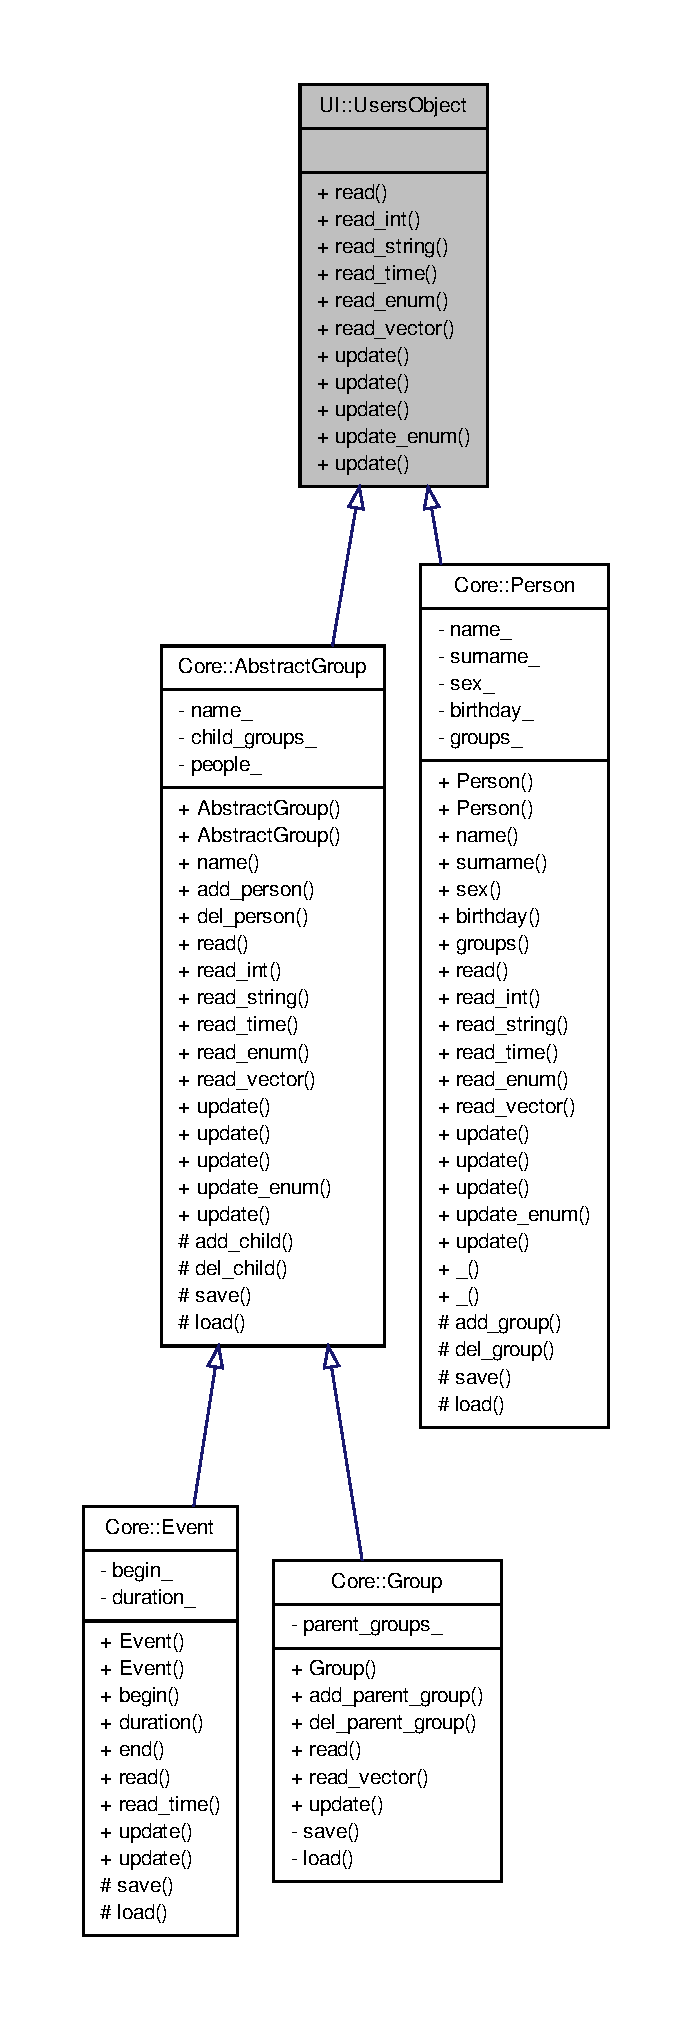
\includegraphics[height=600pt]{df/d9e/classUI_1_1UsersObject__inherit__graph}
\end{center}
\end{figure}
\subsection*{Public Member Functions}
\begin{DoxyCompactItemize}
\item 
virtual const std::string \hyperlink{classUI_1_1UsersObject_a68d5297258a2f4da4ff58f4809690db3}{read} () const =0
\item 
virtual const int \hyperlink{classUI_1_1UsersObject_a63ab79bb54b6134a483b2e384c824c7e}{read\_\-int} (const std::string name) const =0  throw (std::bad\_\-cast)
\item 
virtual const std::string \hyperlink{classUI_1_1UsersObject_aed80fcf20b550a0e3484fbe6beb24c19}{read\_\-string} (const std::string name) const =0  throw (std::bad\_\-cast)
\item 
virtual const time\_\-t \hyperlink{classUI_1_1UsersObject_a490536c477c5a796724ce26fd010c680}{read\_\-time} (const std::string name) const =0  throw (std::bad\_\-cast)
\item 
virtual const std::string \hyperlink{classUI_1_1UsersObject_a20ea26010f60e60f38d380fdaa9240d5}{read\_\-enum} (const std::string name) const =0  throw (std::bad\_\-cast)
\item 
virtual const std::vector$<$ \hyperlink{classUI_1_1UsersObject}{UsersObject} $\ast$ $>$ \hyperlink{classUI_1_1UsersObject_a6899d8a06268abb8f2a13feba9921ce5}{read\_\-vector} (const std::string name) const =0  throw (std::bad\_\-cast)
\item 
virtual void \hyperlink{classUI_1_1UsersObject_a9b30123c0a25a66715bce9a58a27d37e}{update} (const std::string name, const int value)=0  throw (std::bad\_\-cast)
\item 
virtual void \hyperlink{classUI_1_1UsersObject_a4c86312e8400ce3e1b5d2c17552ce5f5}{update} (const std::string name, const std::string value)=0  throw (std::bad\_\-cast)
\item 
virtual void \hyperlink{classUI_1_1UsersObject_add0bfcc5674bd3f56eeb68919c640bb7}{update} (const std::string name, const time\_\-t value)=0  throw (std::bad\_\-cast)
\item 
virtual void \hyperlink{classUI_1_1UsersObject_a925f50c5cb5123a13493f76029ae6f06}{update\_\-enum} (const std::string name, const std::string value)=0  throw (std::bad\_\-cast)
\item 
virtual void \hyperlink{classUI_1_1UsersObject_af4cdeca80652e7c57d34aacc7d0a5dc3}{update} (\hyperlink{classUI_1_1UsersObject}{UsersObject} $\ast$object, const bool linked)=0  throw (std::bad\_\-cast)
\end{DoxyCompactItemize}


\subsection{Member Function Documentation}
\hypertarget{classUI_1_1UsersObject_a68d5297258a2f4da4ff58f4809690db3}{
\index{UI::UsersObject@{UI::UsersObject}!read@{read}}
\index{read@{read}!UI::UsersObject@{UI::UsersObject}}
\subsubsection[{read}]{\setlength{\rightskip}{0pt plus 5cm}virtual const std::string UI::UsersObject::read (
\begin{DoxyParamCaption}
{}
\end{DoxyParamCaption}
) const\hspace{0.3cm}{\ttfamily  \mbox{[}pure virtual\mbox{]}}}}
\label{df/d0b/classUI_1_1UsersObject_a68d5297258a2f4da4ff58f4809690db3}


Implemented in \hyperlink{classCore_1_1AbstractGroup_a0306b58e715d164aef3e29de0ec659bd}{Core::AbstractGroup}, \hyperlink{classCore_1_1Event_a8dd94bcb05cb3c5ef065fa204cd724f9}{Core::Event}, \hyperlink{classCore_1_1Group_a5fe3fef1b6709f953e5487841d90bbb9}{Core::Group}, and \hyperlink{classCore_1_1Person_a3b86cab797444527364376dad2a0c300}{Core::Person}.

\hypertarget{classUI_1_1UsersObject_a20ea26010f60e60f38d380fdaa9240d5}{
\index{UI::UsersObject@{UI::UsersObject}!read\_\-enum@{read\_\-enum}}
\index{read\_\-enum@{read\_\-enum}!UI::UsersObject@{UI::UsersObject}}
\subsubsection[{read\_\-enum}]{\setlength{\rightskip}{0pt plus 5cm}virtual const std::string UI::UsersObject::read\_\-enum (
\begin{DoxyParamCaption}
\item[{const std::string}]{name}
\end{DoxyParamCaption}
) const  throw (std::bad\_\-cast)\hspace{0.3cm}{\ttfamily  \mbox{[}pure virtual\mbox{]}}}}
\label{df/d0b/classUI_1_1UsersObject_a20ea26010f60e60f38d380fdaa9240d5}


Implemented in \hyperlink{classCore_1_1AbstractGroup_a2f373e90feaad172563c6256ae30a6a6}{Core::AbstractGroup}, and \hyperlink{classCore_1_1Person_a5dfa21d7b0a58e09f71e07a4298f0f62}{Core::Person}.

\hypertarget{classUI_1_1UsersObject_a63ab79bb54b6134a483b2e384c824c7e}{
\index{UI::UsersObject@{UI::UsersObject}!read\_\-int@{read\_\-int}}
\index{read\_\-int@{read\_\-int}!UI::UsersObject@{UI::UsersObject}}
\subsubsection[{read\_\-int}]{\setlength{\rightskip}{0pt plus 5cm}virtual const int UI::UsersObject::read\_\-int (
\begin{DoxyParamCaption}
\item[{const std::string}]{name}
\end{DoxyParamCaption}
) const  throw (std::bad\_\-cast)\hspace{0.3cm}{\ttfamily  \mbox{[}pure virtual\mbox{]}}}}
\label{df/d0b/classUI_1_1UsersObject_a63ab79bb54b6134a483b2e384c824c7e}


Implemented in \hyperlink{classCore_1_1AbstractGroup_a7e15ec9b621230659a5ca2f0be724d83}{Core::AbstractGroup}, and \hyperlink{classCore_1_1Person_a9b1601502537f54b7c33fc593f8df590}{Core::Person}.

\hypertarget{classUI_1_1UsersObject_aed80fcf20b550a0e3484fbe6beb24c19}{
\index{UI::UsersObject@{UI::UsersObject}!read\_\-string@{read\_\-string}}
\index{read\_\-string@{read\_\-string}!UI::UsersObject@{UI::UsersObject}}
\subsubsection[{read\_\-string}]{\setlength{\rightskip}{0pt plus 5cm}virtual const std::string UI::UsersObject::read\_\-string (
\begin{DoxyParamCaption}
\item[{const std::string}]{name}
\end{DoxyParamCaption}
) const  throw (std::bad\_\-cast)\hspace{0.3cm}{\ttfamily  \mbox{[}pure virtual\mbox{]}}}}
\label{df/d0b/classUI_1_1UsersObject_aed80fcf20b550a0e3484fbe6beb24c19}


Implemented in \hyperlink{classCore_1_1AbstractGroup_a907fc505a7f7828fcd2e7f6eaf5e27cd}{Core::AbstractGroup}, and \hyperlink{classCore_1_1Person_a4b7d0b1c545c2c4876b3f410b914f3a2}{Core::Person}.

\hypertarget{classUI_1_1UsersObject_a490536c477c5a796724ce26fd010c680}{
\index{UI::UsersObject@{UI::UsersObject}!read\_\-time@{read\_\-time}}
\index{read\_\-time@{read\_\-time}!UI::UsersObject@{UI::UsersObject}}
\subsubsection[{read\_\-time}]{\setlength{\rightskip}{0pt plus 5cm}virtual const time\_\-t UI::UsersObject::read\_\-time (
\begin{DoxyParamCaption}
\item[{const std::string}]{name}
\end{DoxyParamCaption}
) const  throw (std::bad\_\-cast)\hspace{0.3cm}{\ttfamily  \mbox{[}pure virtual\mbox{]}}}}
\label{df/d0b/classUI_1_1UsersObject_a490536c477c5a796724ce26fd010c680}


Implemented in \hyperlink{classCore_1_1AbstractGroup_af52530d29e3b8f0047a0c0675dc6c912}{Core::AbstractGroup}, \hyperlink{classCore_1_1Event_a4977832cb03001d8afe46bcddc60ce1a}{Core::Event}, and \hyperlink{classCore_1_1Person_ad0485ff28f4f80aeb0da9f8a6ae2f6d0}{Core::Person}.

\hypertarget{classUI_1_1UsersObject_a6899d8a06268abb8f2a13feba9921ce5}{
\index{UI::UsersObject@{UI::UsersObject}!read\_\-vector@{read\_\-vector}}
\index{read\_\-vector@{read\_\-vector}!UI::UsersObject@{UI::UsersObject}}
\subsubsection[{read\_\-vector}]{\setlength{\rightskip}{0pt plus 5cm}virtual const std::vector$<${\bf UsersObject} $\ast$$>$ UI::UsersObject::read\_\-vector (
\begin{DoxyParamCaption}
\item[{const std::string}]{name}
\end{DoxyParamCaption}
) const  throw (std::bad\_\-cast)\hspace{0.3cm}{\ttfamily  \mbox{[}pure virtual\mbox{]}}}}
\label{df/d0b/classUI_1_1UsersObject_a6899d8a06268abb8f2a13feba9921ce5}


Implemented in \hyperlink{classCore_1_1AbstractGroup_ab582f4364426a152875742278ba0d999}{Core::AbstractGroup}, \hyperlink{classCore_1_1Group_a52e48b1f92f6354b4e3a32d710b9c7b3}{Core::Group}, and \hyperlink{classCore_1_1Person_ab28c3e468d265c16bce1d4488493c5a6}{Core::Person}.

\hypertarget{classUI_1_1UsersObject_add0bfcc5674bd3f56eeb68919c640bb7}{
\index{UI::UsersObject@{UI::UsersObject}!update@{update}}
\index{update@{update}!UI::UsersObject@{UI::UsersObject}}
\subsubsection[{update}]{\setlength{\rightskip}{0pt plus 5cm}virtual void UI::UsersObject::update (
\begin{DoxyParamCaption}
\item[{const std::string}]{name, }
\item[{const time\_\-t}]{value}
\end{DoxyParamCaption}
)  throw (std::bad\_\-cast)\hspace{0.3cm}{\ttfamily  \mbox{[}pure virtual\mbox{]}}}}
\label{df/d0b/classUI_1_1UsersObject_add0bfcc5674bd3f56eeb68919c640bb7}


Implemented in \hyperlink{classCore_1_1AbstractGroup_a9891a3850584dc3677563aea603fb9c2}{Core::AbstractGroup}, \hyperlink{classCore_1_1Event_aaa4b9def6b65cc896e0054210b2d5dae}{Core::Event}, and \hyperlink{classCore_1_1Person_ad650eba89f671041c26f8d1419f6e6c8}{Core::Person}.

\hypertarget{classUI_1_1UsersObject_af4cdeca80652e7c57d34aacc7d0a5dc3}{
\index{UI::UsersObject@{UI::UsersObject}!update@{update}}
\index{update@{update}!UI::UsersObject@{UI::UsersObject}}
\subsubsection[{update}]{\setlength{\rightskip}{0pt plus 5cm}virtual void UI::UsersObject::update (
\begin{DoxyParamCaption}
\item[{{\bf UsersObject} $\ast$}]{object, }
\item[{const bool}]{linked}
\end{DoxyParamCaption}
)  throw (std::bad\_\-cast)\hspace{0.3cm}{\ttfamily  \mbox{[}pure virtual\mbox{]}}}}
\label{df/d0b/classUI_1_1UsersObject_af4cdeca80652e7c57d34aacc7d0a5dc3}


Implemented in \hyperlink{classCore_1_1AbstractGroup_a1b3a59bf11da1ea7bd9a0735cb54dbb8}{Core::AbstractGroup}, \hyperlink{classCore_1_1Event_a308ae7ad334b8c9a166dc57cfd6a0524}{Core::Event}, and \hyperlink{classCore_1_1Group_a12d2636d65f1baea3666bb492320b5c1}{Core::Group}.

\hypertarget{classUI_1_1UsersObject_a4c86312e8400ce3e1b5d2c17552ce5f5}{
\index{UI::UsersObject@{UI::UsersObject}!update@{update}}
\index{update@{update}!UI::UsersObject@{UI::UsersObject}}
\subsubsection[{update}]{\setlength{\rightskip}{0pt plus 5cm}virtual void UI::UsersObject::update (
\begin{DoxyParamCaption}
\item[{const std::string}]{name, }
\item[{const std::string}]{value}
\end{DoxyParamCaption}
)  throw (std::bad\_\-cast)\hspace{0.3cm}{\ttfamily  \mbox{[}pure virtual\mbox{]}}}}
\label{df/d0b/classUI_1_1UsersObject_a4c86312e8400ce3e1b5d2c17552ce5f5}


Implemented in \hyperlink{classCore_1_1AbstractGroup_a39c1a34ff912b5abd298f58bf6196a45}{Core::AbstractGroup}, and \hyperlink{classCore_1_1Person_a51ec02307587cf9dfd7ed3036cf202cd}{Core::Person}.

\hypertarget{classUI_1_1UsersObject_a9b30123c0a25a66715bce9a58a27d37e}{
\index{UI::UsersObject@{UI::UsersObject}!update@{update}}
\index{update@{update}!UI::UsersObject@{UI::UsersObject}}
\subsubsection[{update}]{\setlength{\rightskip}{0pt plus 5cm}virtual void UI::UsersObject::update (
\begin{DoxyParamCaption}
\item[{const std::string}]{name, }
\item[{const int}]{value}
\end{DoxyParamCaption}
)  throw (std::bad\_\-cast)\hspace{0.3cm}{\ttfamily  \mbox{[}pure virtual\mbox{]}}}}
\label{df/d0b/classUI_1_1UsersObject_a9b30123c0a25a66715bce9a58a27d37e}


Implemented in \hyperlink{classCore_1_1AbstractGroup_a18d88f5abb55fa9c829bf6600be58c90}{Core::AbstractGroup}, and \hyperlink{classCore_1_1Person_ac2900dc24258c00ea1de17350c3f4658}{Core::Person}.

\hypertarget{classUI_1_1UsersObject_a925f50c5cb5123a13493f76029ae6f06}{
\index{UI::UsersObject@{UI::UsersObject}!update\_\-enum@{update\_\-enum}}
\index{update\_\-enum@{update\_\-enum}!UI::UsersObject@{UI::UsersObject}}
\subsubsection[{update\_\-enum}]{\setlength{\rightskip}{0pt plus 5cm}virtual void UI::UsersObject::update\_\-enum (
\begin{DoxyParamCaption}
\item[{const std::string}]{name, }
\item[{const std::string}]{value}
\end{DoxyParamCaption}
)  throw (std::bad\_\-cast)\hspace{0.3cm}{\ttfamily  \mbox{[}pure virtual\mbox{]}}}}
\label{df/d0b/classUI_1_1UsersObject_a925f50c5cb5123a13493f76029ae6f06}


Implemented in \hyperlink{classCore_1_1AbstractGroup_a1f379a7c4d54b49db4d20127521a238a}{Core::AbstractGroup}, and \hyperlink{classCore_1_1Person_a1c6826659c2413189dae536f7c83af98}{Core::Person}.



The documentation for this class was generated from the following file:\begin{DoxyCompactItemize}
\item 
src/include/\hyperlink{usersobject_8h}{usersobject.h}\end{DoxyCompactItemize}

\chapter{File Documentation}
\hypertarget{backend_8cpp}{
\section{src/backend.cpp File Reference}
\label{d6/d84/backend_8cpp}\index{src/backend.cpp@{src/backend.cpp}}
}
{\ttfamily \#include $<$backend.h$>$}\par
Include dependency graph for backend.cpp:
\nopagebreak
\begin{figure}[H]
\begin{center}
\leavevmode
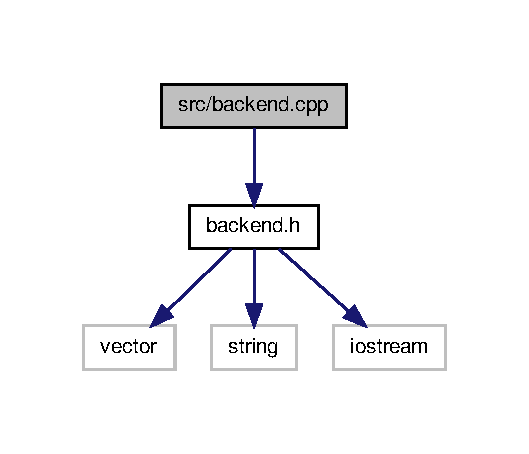
\includegraphics[width=254pt]{da/df1/backend_8cpp__incl}
\end{center}
\end{figure}
\subsection*{Functions}
\begin{DoxyCompactItemize}
\item 
std::vector$<$ \hyperlink{classAbstractBackend}{AbstractBackend} $\ast$ $>$ \& \hyperlink{backend_8cpp_a52651e1c45f0418eb99bf5ac128c6c77}{backends} ()
\end{DoxyCompactItemize}


\subsection{Function Documentation}
\hypertarget{backend_8cpp_a52651e1c45f0418eb99bf5ac128c6c77}{
\index{backend.cpp@{backend.cpp}!backends@{backends}}
\index{backends@{backends}!backend.cpp@{backend.cpp}}
\subsubsection[{backends}]{\setlength{\rightskip}{0pt plus 5cm}std::vector$<${\bf AbstractBackend} $\ast$$>$\& backends (
\begin{DoxyParamCaption}
{}
\end{DoxyParamCaption}
)}}
\label{d6/d84/backend_8cpp_a52651e1c45f0418eb99bf5ac128c6c77}


Here is the call graph for this function:
\nopagebreak
\begin{figure}[H]
\begin{center}
\leavevmode
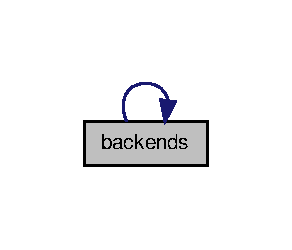
\includegraphics[width=140pt]{d6/d84/backend_8cpp_a52651e1c45f0418eb99bf5ac128c6c77_cgraph}
\end{center}
\end{figure}




Here is the caller graph for this function:
\nopagebreak
\begin{figure}[H]
\begin{center}
\leavevmode
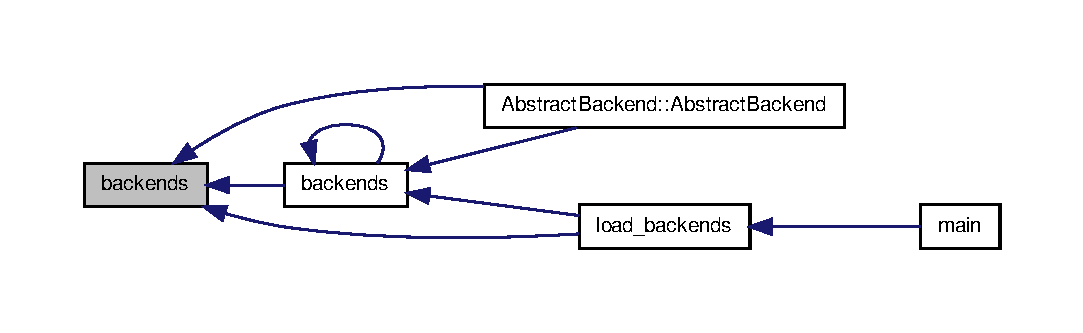
\includegraphics[width=400pt]{d6/d84/backend_8cpp_a52651e1c45f0418eb99bf5ac128c6c77_icgraph}
\end{center}
\end{figure}



\hypertarget{sqlite_8cpp}{
\section{src/backends/storage/sqlite.cpp File Reference}
\label{d9/df4/sqlite_8cpp}\index{src/backends/storage/sqlite.cpp@{src/backends/storage/sqlite.cpp}}
}
{\ttfamily \#include $<$abstractstorage.h$>$}\par
Include dependency graph for sqlite.cpp:
\nopagebreak
\begin{figure}[H]
\begin{center}
\leavevmode
\includegraphics[width=397pt]{d4/df8/sqlite_8cpp__incl}
\end{center}
\end{figure}
\subsection*{Classes}
\begin{DoxyCompactItemize}
\item 
class \hyperlink{classSQLiteStorage}{SQLiteStorage}
\end{DoxyCompactItemize}
\subsection*{Variables}
\begin{DoxyCompactItemize}
\item 
\hyperlink{classSQLiteStorage}{SQLiteStorage} \hyperlink{sqlite_8cpp_ad27658acf383e76886c68086c864b187}{\_\-object}
\end{DoxyCompactItemize}


\subsection{Variable Documentation}
\hypertarget{sqlite_8cpp_ad27658acf383e76886c68086c864b187}{
\index{sqlite.cpp@{sqlite.cpp}!\_\-object@{\_\-object}}
\index{\_\-object@{\_\-object}!sqlite.cpp@{sqlite.cpp}}
\subsubsection[{\_\-object}]{\setlength{\rightskip}{0pt plus 5cm}{\bf SQLiteStorage} {\bf \_\-object}}}
\label{d9/df4/sqlite_8cpp_ad27658acf383e76886c68086c864b187}

\hypertarget{abstractgroup_8cpp}{
\section{src/core/abstractgroup.cpp File Reference}
\label{dd/da0/abstractgroup_8cpp}\index{src/core/abstractgroup.cpp@{src/core/abstractgroup.cpp}}
}
{\ttfamily \#include $<$abstractgroup.h$>$}\par
{\ttfamily \#include $<$sstream$>$}\par
Include dependency graph for abstractgroup.cpp:
\nopagebreak
\begin{figure}[H]
\begin{center}
\leavevmode
\includegraphics[width=400pt]{da/dcb/abstractgroup_8cpp__incl}
\end{center}
\end{figure}

\hypertarget{event_8cpp}{
\section{src/core/event.cpp File Reference}
\label{df/d1b/event_8cpp}\index{src/core/event.cpp@{src/core/event.cpp}}
}
{\ttfamily \#include $<$event.h$>$}\par
{\ttfamily \#include $<$group.h$>$}\par
Include dependency graph for event.cpp:
\nopagebreak
\begin{figure}[H]
\begin{center}
\leavevmode
\includegraphics[width=400pt]{d6/d99/event_8cpp__incl}
\end{center}
\end{figure}

\hypertarget{group_8cpp}{
\section{src/core/group.cpp File Reference}
\label{d3/d97/group_8cpp}\index{src/core/group.cpp@{src/core/group.cpp}}
}
{\ttfamily \#include $<$group.h$>$}\par
Include dependency graph for group.cpp:
\nopagebreak
\begin{figure}[H]
\begin{center}
\leavevmode
\includegraphics[width=178pt]{d0/dca/group_8cpp__incl}
\end{center}
\end{figure}

\hypertarget{person_8cpp}{
\section{src/person.cpp File Reference}
\label{d8/de5/person_8cpp}\index{src/person.cpp@{src/person.cpp}}
}
{\ttfamily \#include $<$person.h$>$}\par

\hypertarget{abstractgroup_8h}{
\section{src/include/abstractgroup.h File Reference}
\label{df/de3/abstractgroup_8h}\index{src/include/abstractgroup.h@{src/include/abstractgroup.h}}
}
{\ttfamily \#include $<$string$>$}\par
{\ttfamily \#include $<$vector$>$}\par
{\ttfamily \#include $<$object.h$>$}\par
{\ttfamily \#include $<$person.h$>$}\par
Include dependency graph for abstractgroup.h:
\nopagebreak
\begin{figure}[H]
\begin{center}
\leavevmode
\includegraphics[width=400pt]{d8/d98/abstractgroup_8h__incl}
\end{center}
\end{figure}
This graph shows which files directly or indirectly include this file:
\nopagebreak
\begin{figure}[H]
\begin{center}
\leavevmode
\includegraphics[width=400pt]{dd/d27/abstractgroup_8h__dep__incl}
\end{center}
\end{figure}
\subsection*{Classes}
\begin{DoxyCompactItemize}
\item 
class \hyperlink{classCore_1_1AbstractGroup}{Core::AbstractGroup}
\begin{DoxyCompactList}\small\item\em Base group functionality. You need to use it instead of \hyperlink{classCore_1_1Group}{Group} or \hyperlink{classCore_1_1Event}{Event} in most cases. \item\end{DoxyCompactList}\end{DoxyCompactItemize}
\subsection*{Namespaces}
\begin{DoxyCompactItemize}
\item 
namespace \hyperlink{namespaceCore}{Core}


\begin{DoxyCompactList}\small\item\em \hyperlink{namespaceCore}{Core} model classes. \item\end{DoxyCompactList}

\end{DoxyCompactItemize}

\hypertarget{abstractstorage_8h}{
\section{src/include/abstractstorage.h File Reference}
\label{de/d16/abstractstorage_8h}\index{src/include/abstractstorage.h@{src/include/abstractstorage.h}}
}
{\ttfamily \#include $<$string$>$}\par
{\ttfamily \#include $<$vector$>$}\par
{\ttfamily \#include $<$typeinfo$>$}\par
{\ttfamily \#include $<$storableobject.h$>$}\par
\subsection*{Classes}
\begin{DoxyCompactItemize}
\item 
class \hyperlink{classStorage_1_1AbstractStorage}{Storage::AbstractStorage}
\begin{DoxyCompactList}\small\item\em Abstract interface for storage. \item\end{DoxyCompactList}\item 
struct \hyperlink{structStorage_1_1AbstractStorage_1_1Argument}{Storage::AbstractStorage::Argument}
\begin{DoxyCompactList}\small\item\em an auxiliary structure to make search query and create objects. \item\end{DoxyCompactList}\end{DoxyCompactItemize}
\subsection*{Namespaces}
\begin{DoxyCompactItemize}
\item 
namespace \hyperlink{namespaceStorage}{Storage}


\begin{DoxyCompactList}\small\item\em \hyperlink{namespaceStorage}{Storage} classes. \item\end{DoxyCompactList}

\end{DoxyCompactItemize}

\hypertarget{abstractui_8h}{
\section{src/include/abstractui.h File Reference}
\label{d1/d7a/abstractui_8h}\index{src/include/abstractui.h@{src/include/abstractui.h}}
}
{\ttfamily \#include $<$usersobject.h$>$}\par
{\ttfamily \#include $<$abstractstorage.h$>$}\par
\subsection*{Classes}
\begin{DoxyCompactItemize}
\item 
class \hyperlink{classUI_1_1AbstractUI}{UI::AbstractUI}
\end{DoxyCompactItemize}
\subsection*{Namespaces}
\begin{DoxyCompactItemize}
\item 
namespace \hyperlink{namespaceUI}{UI}
\end{DoxyCompactItemize}

\hypertarget{backend_8h}{
\section{src/include/backend.h File Reference}
\label{de/d34/backend_8h}\index{src/include/backend.h@{src/include/backend.h}}
}
{\ttfamily \#include $<$vector$>$}\par
{\ttfamily \#include $<$string$>$}\par
{\ttfamily \#include $<$iostream$>$}\par
Include dependency graph for backend.h:
\nopagebreak
\begin{figure}[H]
\begin{center}
\leavevmode
\includegraphics[width=254pt]{d8/d88/backend_8h__incl}
\end{center}
\end{figure}
This graph shows which files directly or indirectly include this file:
\nopagebreak
\begin{figure}[H]
\begin{center}
\leavevmode
\includegraphics[width=400pt]{d7/d18/backend_8h__dep__incl}
\end{center}
\end{figure}
\subsection*{Classes}
\begin{DoxyCompactItemize}
\item 
class \hyperlink{classAbstractBackend}{AbstractBackend}
\end{DoxyCompactItemize}
\subsection*{Functions}
\begin{DoxyCompactItemize}
\item 
std::vector$<$ \hyperlink{classAbstractBackend}{AbstractBackend} $\ast$ $>$ \& \hyperlink{backend_8h_a52651e1c45f0418eb99bf5ac128c6c77}{backends} ()
\end{DoxyCompactItemize}


\subsection{Function Documentation}
\hypertarget{backend_8h_a52651e1c45f0418eb99bf5ac128c6c77}{
\index{backend.h@{backend.h}!backends@{backends}}
\index{backends@{backends}!backend.h@{backend.h}}
\subsubsection[{backends}]{\setlength{\rightskip}{0pt plus 5cm}std::vector$<${\bf AbstractBackend} $\ast$$>$\& backends (
\begin{DoxyParamCaption}
{}
\end{DoxyParamCaption}
)}}
\label{de/d34/backend_8h_a52651e1c45f0418eb99bf5ac128c6c77}


Here is the call graph for this function:
\nopagebreak
\begin{figure}[H]
\begin{center}
\leavevmode
\includegraphics[width=236pt]{de/d34/backend_8h_a52651e1c45f0418eb99bf5ac128c6c77_cgraph}
\end{center}
\end{figure}




Here is the caller graph for this function:
\nopagebreak
\begin{figure}[H]
\begin{center}
\leavevmode
\includegraphics[width=400pt]{de/d34/backend_8h_a52651e1c45f0418eb99bf5ac128c6c77_icgraph}
\end{center}
\end{figure}



\hypertarget{event_8h}{
\section{src/event.h File Reference}
\label{dd/d20/event_8h}\index{src/event.h@{src/event.h}}
}
{\ttfamily \#include $<$string$>$}\par
{\ttfamily \#include $<$vector$>$}\par
{\ttfamily \#include $<$time.h$>$}\par
{\ttfamily \#include $<$types.h$>$}\par
{\ttfamily \#include $<$group.h$>$}\par
{\ttfamily \#include $<$person.h$>$}\par
{\ttfamily \#include $<$calendar.h$>$}\par
\subsection*{Classes}
\begin{DoxyCompactItemize}
\item 
class \hyperlink{classEvent}{Event}
\begin{DoxyCompactList}\small\item\em Class keeps information about event. \item\end{DoxyCompactList}\end{DoxyCompactItemize}

\hypertarget{group_8h}{
\section{src/group.h File Reference}
\label{d9/dd1/group_8h}\index{src/group.h@{src/group.h}}
}
{\ttfamily \#include $<$iostream$>$}\par
{\ttfamily \#include $<$string$>$}\par
{\ttfamily \#include $<$vector$>$}\par
{\ttfamily \#include \char`\"{}types.h\char`\"{}}\par
{\ttfamily \#include \char`\"{}group\_\-content.h\char`\"{}}\par
{\ttfamily \#include \char`\"{}calendar.h\char`\"{}}\par
{\ttfamily \#include \char`\"{}person.h\char`\"{}}\par
\subsection*{Classes}
\begin{DoxyCompactItemize}
\item 
class \hyperlink{classGroup}{Group}
\begin{DoxyCompactList}\small\item\em Class keeps information about group of people. \item\end{DoxyCompactList}\end{DoxyCompactItemize}

\hypertarget{person_8h}{
\section{src/include/person.h File Reference}
\label{d4/d98/person_8h}\index{src/include/person.h@{src/include/person.h}}
}
{\ttfamily \#include $<$string$>$}\par
{\ttfamily \#include $<$sstream$>$}\par
{\ttfamily \#include $<$vector$>$}\par
{\ttfamily \#include $<$object.h$>$}\par
{\ttfamily \#include $<$abstractgroup.h$>$}\par
Include dependency graph for person.h:
\nopagebreak
\begin{figure}[H]
\begin{center}
\leavevmode
\includegraphics[width=400pt]{de/de3/person_8h__incl}
\end{center}
\end{figure}
This graph shows which files directly or indirectly include this file:
\nopagebreak
\begin{figure}[H]
\begin{center}
\leavevmode
\includegraphics[width=400pt]{dc/daa/person_8h__dep__incl}
\end{center}
\end{figure}
\subsection*{Classes}
\begin{DoxyCompactItemize}
\item 
class \hyperlink{classCore_1_1Person}{Core::Person}
\begin{DoxyCompactList}\small\item\em Class keeps person unique data. \item\end{DoxyCompactList}\end{DoxyCompactItemize}
\subsection*{Namespaces}
\begin{DoxyCompactItemize}
\item 
namespace \hyperlink{namespaceCore}{Core}


\begin{DoxyCompactList}\small\item\em \hyperlink{namespaceCore}{Core} model classes. \item\end{DoxyCompactList}

\end{DoxyCompactItemize}

\hypertarget{storableobject_8h}{
\section{src/include/storableobject.h File Reference}
\label{d5/d07/storableobject_8h}\index{src/include/storableobject.h@{src/include/storableobject.h}}
}
{\ttfamily \#include $<$string$>$}\par
{\ttfamily \#include $<$vector$>$}\par
{\ttfamily \#include $<$abstractstorage.h$>$}\par
\subsection*{Classes}
\begin{DoxyCompactItemize}
\item 
class \hyperlink{classStorage_1_1StorableObject}{Storage::StorableObject}
\end{DoxyCompactItemize}
\subsection*{Namespaces}
\begin{DoxyCompactItemize}
\item 
namespace \hyperlink{namespaceStorage}{Storage}


\begin{DoxyCompactList}\small\item\em \hyperlink{namespaceStorage}{Storage} classes. \item\end{DoxyCompactList}

\end{DoxyCompactItemize}

\hypertarget{usersobject_8h}{
\section{src/include/usersobject.h File Reference}
\label{d2/dcb/usersobject_8h}\index{src/include/usersobject.h@{src/include/usersobject.h}}
}
{\ttfamily \#include $<$string$>$}\par
{\ttfamily \#include $<$vector$>$}\par
{\ttfamily \#include $<$typeinfo$>$}\par
Include dependency graph for usersobject.h:
\nopagebreak
\begin{figure}[H]
\begin{center}
\leavevmode
\includegraphics[width=250pt]{db/d06/usersobject_8h__incl}
\end{center}
\end{figure}
This graph shows which files directly or indirectly include this file:
\nopagebreak
\begin{figure}[H]
\begin{center}
\leavevmode
\includegraphics[width=400pt]{df/d4e/usersobject_8h__dep__incl}
\end{center}
\end{figure}
\subsection*{Classes}
\begin{DoxyCompactItemize}
\item 
class \hyperlink{classUI_1_1UsersObject}{UI::UsersObject}
\end{DoxyCompactItemize}
\subsection*{Namespaces}
\begin{DoxyCompactItemize}
\item 
namespace \hyperlink{namespaceUI}{UI}
\end{DoxyCompactItemize}

\hypertarget{main_8cpp}{
\section{src/main.cpp File Reference}
\label{df/d0a/main_8cpp}\index{src/main.cpp@{src/main.cpp}}
}
{\ttfamily \#include $<$iostream$>$}\par
{\ttfamily \#include $<$time.h$>$}\par
{\ttfamily \#include $<$vector$>$}\par
{\ttfamily \#include $<$types.h$>$}\par
{\ttfamily \#include $<$event\_\-template.h$>$}\par
{\ttfamily \#include $<$queue.h$>$}\par
{\ttfamily \#include $<$commands.h$>$}\par
{\ttfamily \#include $<$userinterface.h$>$}\par
{\ttfamily \#include $<$person.h$>$}\par
{\ttfamily \#include $<$group.h$>$}\par
{\ttfamily \#include $<$event.h$>$}\par
{\ttfamily \#include $<$data\_\-storage.h$>$}\par
{\ttfamily \#include $<$file\_\-storage.h$>$}\par
\subsection*{Functions}
\begin{DoxyCompactItemize}
\item 
int \hyperlink{main_8cpp_a0ddf1224851353fc92bfbff6f499fa97}{main} (int argc, char $\ast$argv\mbox{[}$\,$\mbox{]})
\end{DoxyCompactItemize}


\subsection{Function Documentation}
\hypertarget{main_8cpp_a0ddf1224851353fc92bfbff6f499fa97}{
\index{main.cpp@{main.cpp}!main@{main}}
\index{main@{main}!main.cpp@{main.cpp}}
\subsubsection[{main}]{\setlength{\rightskip}{0pt plus 5cm}int main (
\begin{DoxyParamCaption}
\item[{int}]{argc, }
\item[{char $\ast$}]{argv\mbox{[}$\,$\mbox{]}}
\end{DoxyParamCaption}
)}}
\label{df/d0a/main_8cpp_a0ddf1224851353fc92bfbff6f499fa97}

\hypertarget{abstractstorage_8cpp}{
\section{src/storage/abstractstorage.cpp File Reference}
\label{d2/df5/abstractstorage_8cpp}\index{src/storage/abstractstorage.cpp@{src/storage/abstractstorage.cpp}}
}
{\ttfamily \#include $<$abstractstorage.h$>$}\par
Include dependency graph for abstractstorage.cpp:
\nopagebreak
\begin{figure}[H]
\begin{center}
\leavevmode
\includegraphics[width=234pt]{dd/d44/abstractstorage_8cpp__incl}
\end{center}
\end{figure}

\hypertarget{storableobject_8cpp}{
\section{src/storage/storableobject.cpp File Reference}
\label{d3/de7/storableobject_8cpp}\index{src/storage/storableobject.cpp@{src/storage/storableobject.cpp}}
}
{\ttfamily \#include $<$storableobject.h$>$}\par

\hypertarget{architecture__with__backends_8cpp}{
\section{src/tests/architecture\_\-with\_\-backends.cpp File Reference}
\label{d5/dcf/architecture__with__backends_8cpp}\index{src/tests/architecture\_\-with\_\-backends.cpp@{src/tests/architecture\_\-with\_\-backends.cpp}}
}
{\ttfamily \#include $<$abstractstorage.h$>$}\par
{\ttfamily \#include $<$abstractui.h$>$}\par
{\ttfamily \#include $<$backend.h$>$}\par
{\ttfamily \#include $<$iostream$>$}\par
Include dependency graph for architecture\_\-with\_\-backends.cpp:
\nopagebreak
\begin{figure}[H]
\begin{center}
\leavevmode
\includegraphics[width=400pt]{d8/d29/architecture__with__backends_8cpp__incl}
\end{center}
\end{figure}
\subsection*{Functions}
\begin{DoxyCompactItemize}
\item 
bool \hyperlink{architecture__with__backends_8cpp_a8b3ddd91124b7bb8c0b91c530505dd60}{load\_\-backends} (\hyperlink{classStorage_1_1AbstractStorage}{Storage::AbstractStorage} $\ast$$\ast$storage, \hyperlink{classUI_1_1AbstractUI}{UI::AbstractUI} $\ast$$\ast$ui, std::vector$<$ std::string $>$ \&args)
\item 
int \hyperlink{architecture__with__backends_8cpp_a0ddf1224851353fc92bfbff6f499fa97}{main} (int argc, char $\ast$argv\mbox{[}$\,$\mbox{]})
\end{DoxyCompactItemize}


\subsection{Function Documentation}
\hypertarget{architecture__with__backends_8cpp_a8b3ddd91124b7bb8c0b91c530505dd60}{
\index{architecture\_\-with\_\-backends.cpp@{architecture\_\-with\_\-backends.cpp}!load\_\-backends@{load\_\-backends}}
\index{load\_\-backends@{load\_\-backends}!architecture_with_backends.cpp@{architecture\_\-with\_\-backends.cpp}}
\subsubsection[{load\_\-backends}]{\setlength{\rightskip}{0pt plus 5cm}bool load\_\-backends (
\begin{DoxyParamCaption}
\item[{{\bf Storage::AbstractStorage} $\ast$$\ast$}]{storage, }
\item[{{\bf UI::AbstractUI} $\ast$$\ast$}]{ui, }
\item[{std::vector$<$ std::string $>$ \&}]{args}
\end{DoxyParamCaption}
)}}
\label{d5/dcf/architecture__with__backends_8cpp_a8b3ddd91124b7bb8c0b91c530505dd60}


Here is the call graph for this function:
\nopagebreak
\begin{figure}[H]
\begin{center}
\leavevmode
\includegraphics[width=308pt]{d5/dcf/architecture__with__backends_8cpp_a8b3ddd91124b7bb8c0b91c530505dd60_cgraph}
\end{center}
\end{figure}


\hypertarget{architecture__with__backends_8cpp_a0ddf1224851353fc92bfbff6f499fa97}{
\index{architecture\_\-with\_\-backends.cpp@{architecture\_\-with\_\-backends.cpp}!main@{main}}
\index{main@{main}!architecture_with_backends.cpp@{architecture\_\-with\_\-backends.cpp}}
\subsubsection[{main}]{\setlength{\rightskip}{0pt plus 5cm}int main (
\begin{DoxyParamCaption}
\item[{int}]{argc, }
\item[{char $\ast$}]{argv\mbox{[}$\,$\mbox{]}}
\end{DoxyParamCaption}
)}}
\label{d5/dcf/architecture__with__backends_8cpp_a0ddf1224851353fc92bfbff6f499fa97}


Here is the call graph for this function:
\nopagebreak
\begin{figure}[H]
\begin{center}
\leavevmode
\includegraphics[width=382pt]{d5/dcf/architecture__with__backends_8cpp_a0ddf1224851353fc92bfbff6f499fa97_cgraph}
\end{center}
\end{figure}



\hypertarget{model__classes__are__real_8cpp}{
\section{src/tests/model\_\-classes\_\-are\_\-real.cpp File Reference}
\label{df/d1b/model__classes__are__real_8cpp}\index{src/tests/model\_\-classes\_\-are\_\-real.cpp@{src/tests/model\_\-classes\_\-are\_\-real.cpp}}
}
{\ttfamily \#include $<$abstractstorage.h$>$}\par
{\ttfamily \#include $<$person.h$>$}\par
{\ttfamily \#include $<$group.h$>$}\par
{\ttfamily \#include $<$event.h$>$}\par
Include dependency graph for model\_\-classes\_\-are\_\-real.cpp:
\nopagebreak
\begin{figure}[H]
\begin{center}
\leavevmode
\includegraphics[width=376pt]{d6/d84/model__classes__are__real_8cpp__incl}
\end{center}
\end{figure}
\subsection*{Classes}
\begin{DoxyCompactItemize}
\item 
class \hyperlink{classDummyStorage}{DummyStorage}
\end{DoxyCompactItemize}
\subsection*{Functions}
\begin{DoxyCompactItemize}
\item 
int \hyperlink{model__classes__are__real_8cpp_ae66f6b31b5ad750f1fe042a706a4e3d4}{main} ()
\end{DoxyCompactItemize}


\subsection{Function Documentation}
\hypertarget{model__classes__are__real_8cpp_ae66f6b31b5ad750f1fe042a706a4e3d4}{
\index{model\_\-classes\_\-are\_\-real.cpp@{model\_\-classes\_\-are\_\-real.cpp}!main@{main}}
\index{main@{main}!model_classes_are_real.cpp@{model\_\-classes\_\-are\_\-real.cpp}}
\subsubsection[{main}]{\setlength{\rightskip}{0pt plus 5cm}int main (
\begin{DoxyParamCaption}
{}
\end{DoxyParamCaption}
)}}
\label{df/d1b/model__classes__are__real_8cpp_ae66f6b31b5ad750f1fe042a706a4e3d4}


Here is the call graph for this function:
\nopagebreak
\begin{figure}[H]
\begin{center}
\leavevmode
\includegraphics[width=400pt]{df/d1b/model__classes__are__real_8cpp_ae66f6b31b5ad750f1fe042a706a4e3d4_cgraph}
\end{center}
\end{figure}



\hypertarget{abstractui_8cpp}{
\section{src/core/abstractui.cpp File Reference}
\label{d6/df7/abstractui_8cpp}\index{src/core/abstractui.cpp@{src/core/abstractui.cpp}}
}
{\ttfamily \#include $<$abstractui.h$>$}\par
{\ttfamily \#include $<$yaml-\/cpp/yaml.h$>$}\par
Include dependency graph for abstractui.cpp:
\nopagebreak
\begin{figure}[H]
\begin{center}
\leavevmode
\includegraphics[width=254pt]{df/d4b/abstractui_8cpp__incl}
\end{center}
\end{figure}

\hypertarget{usersobject_8cpp}{
\section{src/ui/usersobject.cpp File Reference}
\label{d1/d88/usersobject_8cpp}\index{src/ui/usersobject.cpp@{src/ui/usersobject.cpp}}
}
{\ttfamily \#include $<$usersobject.h$>$}\par

\printindex
\end{document}
